% Main source file

\documentclass[a4paper,11pt]{book}
\usepackage[UKenglish]{babel}

\usepackage[T1]{fontenc}
\usepackage[utf8]{inputenc}
\usepackage{graphicx}
\usepackage{calc}
\usepackage{amsmath}
\usepackage{hyperref}
\usepackage{aas_macros}
% Stuff that might be useful depending on individual needs
\usepackage{array}
\usepackage{boxedminipage}
\usepackage{rotating}
\usepackage{amssymb}
\usepackage{subfigure}
\usepackage{hhline}
\usepackage{moreverb}
\usepackage{float}
\usepackage{tikz}
\usepackage{tikz-3dplot}
\usetikzlibrary{angles,quotes}
\usetikzlibrary{shapes.geometric}
\let\vec\mathbf

%DIN TITTEL HER:
\newcommand{\mintittel}{Masteroppgave}
\title{\mintittel}
\author{Håkon Tansem}
\date{\today}

% Setting for layout
\setlength{\textwidth}{14.5cm}
\setlength{\headheight}{13.6pt}
\setlength{\marginparwidth}{0.7cm}
%\setlength{\marginparsep}{0.7cm}
\setlength{\evensidemargin}{1cm}

% Fancy heading -  if you want it
\usepackage{fancyhdr}
\pagestyle{fancyplain}
\addtolength{\headwidth}{\marginparsep}
\addtolength{\headwidth}{\marginparwidth}
\renewcommand{\chaptermark}[1]%
	{\markboth{#1}{}}
\renewcommand{\sectionmark}[1]%
	{\markright{\thesection\ #1}}
\lhead[\fancyplain{}{\bfseries\thepage}]%
	{\fancyplain{}{\bfseries\rightmark}}
\rhead[\fancyplain{}{\bfseries\leftmark}]%
	{\fancyplain{}{\bfseries\thepage}}
\cfoot{}

% Below: depends on package float
% -----------------------------------------------------
% Definitions for algorithms
\floatstyle{boxed}
\newfloat{algorithm}{hbt}{loa}[chapter]
\floatname{algorithm}{Algorithm}

%\setcounter{secnumdepth}{3}
%New commands;

\renewcommand{\H}{\mathcal{H}}
\newcommand{\phid}{\dot{\phi}}
\newcommand{\phidd}{\ddot{\phi}}
\newcommand{\Phid}{\dot{\Phi}}
\newcommand{\Phidd}{\ddot{\Phi}}
\newcommand{\psid}{\dot{\psi}}
\newcommand{\Psid}{\dot{\Psi}}
\newcommand{\Psidd}{\ddot{\Psi}}
\newcommand{\R}{\mathcal{R}}
\renewcommand{\L}{\mathcal{L}}
\newcommand{\Rd}{\dot{\mathcal{R}}}
\newcommand{\M}{m_{Pl}}
\newcommand{\g}{g_{\mu\nu}}
\newcommand{\gu}{g^{\mu\nu}}
\newcommand{\Ricci}{R_{\mu\nu}}
\newcommand{\G}{G_{\mu\nu}}
\newcommand{\addotoa}{\dfrac{\ddot{a}}{a}}
\renewcommand{\dh}{\dot{h}}
\newcommand{\ddh}{\ddot{h}}
\newcommand{\dF}{\dot{F}}
\newcommand{\ddF}{\ddot{F}}
\newcommand{\dFoF}{\dfrac{\dF}{F}}
\newcommand{\ddFoF}{\dfrac{\ddF}{F}}
\newcommand{\synch}{\left(\delta_{ij}+h_{ij}\right)}
%\newcommand{\Chr}[2]{\Gamma_{#1}^{#2}


\newcommand{\tphi}{\tilde{\phi}}
\newcommand{\tpsi}{\tilde{\psi}}
\newcommand{\tdpsi}{\dot{\tilde{\psi}}}
\newcommand{\tPhi}{\tilde{\Phi}}
\newcommand{\tdPhi}{\dot{\tilde{\Phi}}}
\newcommand{\tPsi}{\tilde{\Psi}}
\newcommand{\tdPsi}{\dot{\tilde{\Psi}}}
\newcommand{\tE}{\tilde{E}}
\newcommand{\tB}{\tilde{B}}
\newcommand{\tg}{\tilde{g}}
\newcommand{\tV}{\tilde{V}}
\newcommand{\tT}{\tilde{T}}
\newcommand{\tNabla}{\tilde{\nabla}}
\newcommand{\tR}{\tilde{\rho}}
\newcommand{\ta}{\tilde{a}}
\newcommand{\trho}{\tilde{\rho}}
\newcommand{\tP}{\tilde{p}}
\newcommand{\tp}{\tilde{p}}
\newcommand{\tz}{\tilde{z}}
\newcommand{\teta}{\tilde{\eta}}
\renewcommand{\th}{\tilde{h}}
\newcommand{\tH}{\tilde{\mathcal{H}}}
\newcommand{\tdelta}{\tilde{\delta}}
\newcommand{\tv}{\tilde{v}}
\newcommand{\tw}{\tilde{w}}
\newcommand{\taddotoa}{\dfrac{\ddot{\ta}}{\ta}}
\newcommand{\tsynch}{\left(\delta_{ij}+\th_{ij}\right)}
\newcommand{\tOmega}{\tilde{\Omega}}
\newcommand{\C}{\mathcal{C}}

\newcommand{\tabb}[1]{Table \ref{#1}}
\newcommand{\fig}[1]{Figure \ref{#1}}
\newcommand{\eq}[1]{equation (\ref{#1})}
\newcommand{\chap}[1]{Chapter \ref{#1}}
\renewcommand{\sec}[1]{\S\ref{#1}}
\newcommand{\eqs}[2]{equations \eqref{#1} - \eqref{#2}}
\renewcommand{\t}[1]{\mathrm{#1}}
\renewcommand{\k}{{\boldsymbol{k}}}
\newcommand{\K}{(k_1+k_2+k_3)}
%\renewcommand{\sum}{\displaystyle\sum}

\newcommand{\be}{\begin{equation}}
\newcommand{\ee}{\end{equation}}
\newcommand{\ba}{\begin{align}}
\newcommand{\ea}{\end{align}}
\newcommand{\I}{\Bigg|}
\newcommand{\bea}{\begin{eqnarray}}
\newcommand{\eea}{\end{eqnarray}}
\newcommand{\bdm}{\begin{displaymath}}
\newcommand{\edm}{\end{displaymath}}
\newcommand{\beas}{\begin{eqnarray*}}
\newcommand{\eeas}{\end{eqnarray*}}

\newcommand{\khv}{\hat{\mathbf{k}}}
\newcommand{\nhv}{\hat{\mathbf{n}}}
\newcommand{\kh}{\hat{k}}

\newcommand{\av}[1]{\left< #1\right>}
\newcommand{\kv}{\mathbf{k}}
\newcommand{\kdv}{\mathbf{k}'}
\newcommand{\pv}{\mathbf{p}}
\newcommand{\pdv}{\mathbf{p}'}
\newcommand{\qv}{\mathbf{q}}
\newcommand{\qdv}{\mathbf{q}'}
\newcommand{\kmkd}{\mathbf{k}-\mathbf{k}'}
\newcommand{\pmpd}{\mathbf{p}-\mathbf{p}'}
\newcommand{\qmqd}{\mathbf{q}-\mathbf{q}'}
\newcommand{\ppkd}{\mathbf{p}+\mathbf{k}'}
\newcommand{\qpkd}{\mathbf{q}+\mathbf{k}'}
\newcommand{\Pow}[1]{\mathcal{P}\left(#1\right)}
\newcommand{\Pro}[3]{P_{#1 #2}\left( #3\right)}
\newcommand{\dk}{\frac{d^3\kv}{(2\pi)^3}}
\newcommand{\dkd}{\frac{d^3\kv'}{(2\pi)^3}}

% Einstein frame quantities

\newcommand{\tq}{\tilde{q}}
\newcommand{\tpi}{\tilde{\pi}}
\newcommand{\tDelta}{\tilde{\Delta}}

\newcommand{\cssq}{c_s^{\phantom{s}2}}
\newcommand{\tcssq}{\tilde{c}_s^{\phantom{s}2}}
%Fixing height of tables
\renewcommand{\arraystretch}{1.8}

%Wigner symbols
\newcommand{\wignertre}[2]{\genfrac{(}{)}{0pt}{}{#1}{#2}}
\newcommand{\wignersix}[2]{\genfrac{\{}{\}}{0pt}{}{#1}{#2}}
%============================================================
\begin{document}
\pagenumbering{roman}
%\pagestyle{plain}
\begin{titlepage}
\begin{center}

\bfseries
\huge%\LARGE
\mintittel

\vspace{2cm}
\LARGE
Håkon Tansem


\vspace{1cm}
\begin{figure}[h]
\centering
\includegraphics[width=7cm]{uiologo.eps}
\centering
\end{figure}
\vspace{3cm}
\Large
Thesis submitted for the degree of \\
Master of Science in Astronomy%Master of Science Thesis by\\
%\Large
%Amir Hammami\\

\vspace{0.8cm}
\large
Institute of Theoretical Astrophysics\\
University of Oslo

\vspace{0.8cm}
DIN DATO

\end{center}
\normalfont

\end{titlepage}

\vspace*{18cm}
\noindent Copyright \copyright$\,$ 2021, Håkon Tansem
\vspace{4mm}

\noindent This work, entitled ``\mintittel'' is distributed under the
terms of the Public Library of Science Open Access License, a copy of which can be found at
http://www.publiclibraryofscience.org.

\chapter*{Abstract}
\addcontentsline{toc}{chapter}{\numberline{}Abstract}
The large scale structure of the universe provides independent sets of experiments for extracting information about cosmological parameters. Due to redshift space distortions, anisotropy is introduced when observing the matter distribution in the universe.
Future cosmological surveys, such as Euclid, is expected to greatly increase the number of galaxies having their redshifts measured thereby increasing the size of datasets. In preparation for conducting analysis on future datasets, methodology has to be thoroughly tested in order to extract as much information cosmological information from the density field as possible.\\\indent
In this thesis I derive and implement a model for the radial velocity of matter around cosmological filaments using linear perturbation theory. I will also implement and test a proposed improvement to the radial velocity of matter surrounding voids\cite{Achitouv_streaming}. This model, together with the regular radial velocity derived from linear theory, will be implemented into the void-galaxy cross correlation function in redshift space using a linear bias approximation for the overdensity profile. In addition, the regular radial velocity proposed by linear theory will also be implemented for into the void-galaxy cross correlation function in redshift space using an arbitrary dark matter overdensity profile. This dark matter profile will then be scaled in the radial direction introducing an $r_{scale}$ parameter and the amplitude is scaled by $f\sigma_8$. Using The Big MultiDark Planck simulation (BigMDPL)\cite{Multidark_dataset}, I will compare these models with data from numerical calculations and assess their performance. For the analysis conducted on voids, fits to the dataset was performed for the void-galaxy cross correlation function in redshift space. 
\\\indent
I find the model to provide promising results when predicting the radial velocity of matter around cosmological filaments. Although the amplitude of the velocity predicted by linear theory is not entirely accurate, it manages to replicate the shape of the radial velocity derived from the dataset. When applying fits to the void-galaxy correlation function in redshift space, I find the regular velocity model derived from linear theory to perform consistently better than the model with the proposed improvement when fitting $\epsilon$. Applying cuts to the dataset, including only voids with an effective radius $r>40$Mpc/h, i find the regular model to also perform better when fitting the $\beta$ parameter. Lastly, I find the parameter fits to the model using the dark matter overdensity profile to consistently provide accurate fits for $\epsilon$. However, the model does not provide accurate fits for the $f\sigma_8$ even with cuts applied.
\\\indent
\include{acknowledgement}
%\addcontentsline{toc}{chapter}{\numberline{}Contents}
\tableofcontents

\addcontentsline{toc}{chapter}{\numberline{}List of Figures}
\listoffigures
\newpage
\thispagestyle{empty}
\mbox{}

\newpage
\pagestyle{fancyplain}
\pagenumbering{arabic}


%Her har jeg kommentert ut mine delkapitler, denne malen fungerer slik at jeg har ett hoveddokument, som heter main.tex. I denne har jeg \include{navn på en annen .tex fil jeg ønsker at skal bli en del
% av dette dokumentet}. Dvs at i mitt tilfelle hadde jeg en main.tex, sammen med introduction.tex, cosmology.tex, fRgrav.tex osv.

\chapter{Introduction}
The current dominating model for the universe is the $\Lambda CDM$ model. This model assumes that the mass-energy density of the universe is made up of three major components, namely dark energy $\Lambda$, cold dark matter CDM and regular baryonic matter. The modelling of the evolution and expansion of the universe is related to the mass-energy density of the universe itself. An important aspect of cosmology is therefore to constrain the bounds on these components in order to figure out how large the fraction of the total mass-energy density of the universe each of them make up.\\\indent
The leading expirements related to constraining cosmological parameters is the study of radiation remnant from the very early universe, namely the cosmological microwave background (CMB)\cite{1965cmb}, with the COBE-\cite{Smoot_1999} WMAP-\cite{Wmap} and Planck-satellites\cite{planckvi} in the forefront. Other studies include that of stellar supernova type-Ia explosions\cite{Pantheon}. Advances in cosmological experiments over the last decades has brought cosmology into the era of "precision cosmology", now that cosmological parameters can be constrained with sub-percent accuracy. This has lead to tensions in that certain experiments may disagree over values for cosmological parameters. An example of this is the Hubble tension in which measurements of the CMB disagree with that of type Ia supernovae when measuring the evolution of the Hubble parameter, in which quantifies the expansion of the universe. This particular tension could be a case of statistical fluctuation or systematic error, but these situations do warrant more independent experiments in order to strengthen the current knowledge.\\\indent Additional independent set of experiments relating cosmological components to observables can be found through studies of the distribution of matter in the universe, namely the large scale structure (LSS) of the universe. Studies of the large scale structure of the universe include the study of how matter is clustered at different cosmological redshifts in order to determine statistical properties of the matter distribution. On large scales the matter distribution in the universe form a web like pattern known as the cosmic web\cite{bondweb}. Substructures of the cosmic web include voids, empty regions of space containing little to no matter. These voids are bound by structures known as filaments. Filaments consists of gravitationally bound galaxy clusters. Studies like \cite{BeyondBAO}\cite{Nadathur_2020} have shown that the studies the statistical distribution of matter around voids is a useful addition to the current expirements for studying properties of the universe. In addition other studies like \cite{refId0} show that the statistical properties of galaxy clustering provides useful insight. \\\indent
One of the main statistical properties of the LSS that one can measure is the angular correlation function between definable physical objects. In short a correlation function in this context measures the excess probability over random that two objects are separated by a distance $r$. The fact that the universe is expanding\cite{Hubble168} causes light travelling towards us to be redshifted. With current observational experiments, the only reliable way to observe the LSS is through observations of electromagnetic radiation. When observing objects in the universe, the redshifted light causes the observed matter distribution to appear distorted along the line of sight direction. Work on understanding the effects of redshift space distortions on the void galaxy cross correlation function has been conducted \cite{Nadathur_corr}. The imprints of baryonic acoustic oscillations on the correlation between galaxy pairs\cite{pe00300h}, which appear as ripples in the density distribution of baryonic matter, serve as a standard ruler when measuring cosmological parameters. The effects on the the correlation function between matter has been studied both theoretically\cite{peebles1980} and through observational experiments\cite{Eisenstein_2005}. \\\indent
The filaments themselves have not yet received the proper treatment as that of voids and galaxy clusters. Although great efforts have been made analysing many of their properties\cite{Libeskind_2017}, their matter distribution has not yet recieved a thorough statistical review as that of voids and the matter distribution in general. Further contributions to this field includes proper modelling of the physical behaviour, such as the velocity field, of matter around filaments. Using data from the The Big MultiDark Planck simulation (BigMDPL)\cite{Multidark_dataset}, the first part of this work contains an analysis of filaments where the goal is to test a model for the velocity component of dark matter halos perpendicual to the filament spine. Using linear perturbation theory I will derive a simple model for the radial velocity perpendicular to the spine of cosmological filaments. This model will be compared to velocity data from numerical simulations in order to test wether this is a valid approximation for it to be used in further modelling of the statistical properties of filaments.\\\indent
Current surveys of the large scale structure of the universe include the Sloan Digital Sky Survey \cite{Eisenstein_2011} in which the redshifts of $1.5$ million galaxies is measured. Future surveys include the Euclid mission, in which one of the scientific goals is to measure the redshifts upwards of $50$ million galaxies\cite{eucliddefinition}. In preparation for future experiments, like Euclid in which will greatly improve the data for which LSS studies are to be carried out on, simulation data is useful for testing and developing methodology. Current computer simulations enables the study of the evolution of billions of dark matter particles\cite{Millennium}\cite{Multidark_dataset} which allows for relatively accurate representations of the real universe. As mentioned the correlation function for voids and galaxies has been studied in previous works. However in preparation for future observational experiments applying methodology on large datasets provides useful testing. The second part of this thesis includes a test of the void-galaxy correlation function applied on data from the The Big MultiDark Planck simulation (BigMDPL)\cite{Multidark_dataset}. The methodology will be tested using three different samples with different a different number of dark matter halos ranging from $3.5$ million to $15$ million. In addition proposed improvements to the modelling of velocities of matter around voids\cite{Achitouv_streaming} will be tested in order to see if this will improve the performance of the models.\\\indent
This thesis is divided into multiple parts. Chapter \ref{sec:backgroundtheory} provides a summary of cosmological theory used in development of the methodology. It also provides a short summary of the fundemantal statistical theory used and cosmological simulations in general. Chapter \ref{sec:codesused} provides an introduction to the codes utilized for identifying filaments and voids from the simulated distribution of dark matter halos. This is followed by a short introduction of the dataset and its properties given in chapter \ref{sec:dataset}. The methodology particular to the work conducted in this thesis itself is introduced in chapter \ref{sec:method}. This is followed chapter \ref{sec:results} which presents the results and a discussion of their properties. This section is split into two parts. Section \ref{sec:filaments} provides the results and a discussion for the work done on filaments while section \ref{sec:void} provides the same for the work done on voids. 
\chapter{Background Theory}
\section{History of cosmology and how we model the universe}
Skrive noe generelle ting om kosmologi og astronomi historie her.\\

The following subsections are largely based on \cite[ch.7]{schneider2006extragalactic}, \cite[ch.2]{Dodelson:1282338} and \cite{ryden2017introduction} unless otherwise noted.
\subsection{Distances in the universe and cosmological redshift}\label{sec:sec_distance}
Distances in an expanding universe can prove hard to fathom. In our everyday
lives we are used to measuring distances in meters and kilometers. The
average distance from the earth to the sun however is approximately $1.49\cdot10^{11}$m.
Allthough this distance on a cosmic scale is very short, the numbers in our
everyday units of measurement already start to become too big for us to have a
reasonable idea of how long this distance actually is. We have a clear idea of
what a meter and a kilometer is as we have to deal with them everyday. To make
things more manageable when measuring these large distances the average distance
from the earth to the sun has become its own distance unit known as the
Astronomical unit (AU). This unit is a great tool for measuring relative
distances in our own solar system, but our nearest star, Proxima Centauri, is
located at approximately $268394$AU away from our closest star the Sun.
Therefore it is convenient to introduce another unit of distance measurement known as light year. This unit with a value of $9.4607\cdot10^{15}$m is the distance at
which light travels in vacuum during one Julian year equal to $365.25$ days.
This gives us a more manageable account of the distance from the Sun to Proxima
Centauri as $4.244$ light years. With both the AU and the light year introduced
we can define the last unit of measuring distance, namely the parsec equal to $3.26$
light years. One parsec is equal to the distance at which $1$ AU subtends an angle
of one arcsecond (setningen er lik paa wikipedia og Barbara ryden). Most
cosmological distances are measured in parsec, abbreviated Pc, with either the
prefix mega or giga as cosmology deals mostly with intergalactic scales much
larger than the average distance between two galaxies.\\

Due to the fact that the universe is expanding, light traveling towards us from
far away objects gets redshifted. Since the expansion of the universe is
isotropic, i.e, the expansion rate of the universe is equal in all directions,
the redshift of this light can be used to measure the distance at which we
observe objects in the universe. The cosmic redshift $z$ is given by the
relation
\begin{equation}
    z = \frac{\lambda_{obs}}{\lambda_{em}} - 1,
\end{equation}
where $\lambda_{obs}$ is the observed wavelength we measure here on earth and
$\lambda_{em}$ is the wavelength emitted by the observed object. by combining this with the doppler formula
$\frac{\lambda_{obs}-\lambda_{em}}{\lambda_{em}} = \frac{v}{c}$, one gets
\begin{equation}
    z = \frac{v}{c},
\end{equation}
where $v$ is the velocity of the observed object relative to the observer. The
velocity of an object due to the expansion of the universe is given by Hubbles law
\begin{equation}
    v = H_0 d_p,
\end{equation}
where $d_p$ is what is known as proper distance and $H_0$ is the Hubble
parameter at present time. The Hubble parameter measures the expansion rate of
the universe as a function of time. (Kanskje prate om verdien av H0). Proper distance can be interpreted as the length measured if one
was to use a ruler between two objects $a$ and $b$ at a fixed time $t$ taking
into account the fact that our universe is expanding. Before introducing how proper distance is calculated it can be
useful to talk about the concept of comoving distance first. If we choose a time
$t=t_0$, which is present time, and introduce a coordinate system at this time,
we can choose an arbitrary point to center ourselves in in this coordinate
system. If we apply a ruler in this coordinate system and measure the distance
from our point to another arbitrary point, this is the comoving distance $r$.
The comoving distance remains constant through time as the universe expands. The
comoving distance is simply the distance measured in a coordinate system at
$t=t_0$ (dette er kanskje en krokete formulering $d_c$). The proper distance on the other hand factors in the expansion of the
universe through the scale factor $a(t)$. The proper distance is given as
\begin{equation}
    d_p = \int_{r_0}^{r_1}a(t)rdr,
\end{equation}
Where $a(t)$ is a quantity known as the scale factor. The scale factor parametrises the relative expansion of the
universe. It is defined in such a way that $a_0$, subscript $0$ meaning
$a(t=t_0)$ where $t_0$ is present time, is equal to one. This definition of
proper distance also implies that comoving distance is the proper distance at $t=t_0$.
With these properties in place we can now see how redshift, which is a
measurable quantity, can be used to measure the real distance to objects in our universe.\\

Another measurable measurable quantity is flux emitted from an astronomical object.
The flux $F$ is defined as
\begin{equation}
    F = \frac{L}{4\pi R^2},
\end{equation}
where $L$ is the luminosity and $R$ is the distance to the object. Luminosity is a measure
of the absolute electromagnetic power emitted from an astronomical object. The flux however, measured in $W/m^2$, is simply the luminosity
divided by the area of a shell with a radius at which we observe the object, assuming the radiation is isotropically emitted. Some astronomical phenomena, like a type 1a supernova, have a fixed luminosity
due to the characteristics of the process that creates it. This is called a standard candle. By measuring the observed flux from such a phenomena, one can then
calculate the the luminosity distance as 
\begin{equation}
    d_L = \sqrt{\frac{L}{4\pi F}}.
\end{equation}
(Kanskje si noe mer om svakheter med denne.)


\subsection{Modelling the evolution of the universe and the $\Lambda$CDM model}
The cosmological principle states that on sufficiently
large scales the universe is isotropic and homogenous. This means the universe
looks the same in every direction for every observer at any point in space for
sufficiently large scales. By sufficiently large scales one means
distances roughly $100$Mpc or larger \cite[p.~12]{ryden2017introduction}. This has been proved to be a good
assumption by surveys like the Sloan sky survey (svak formulering. Trenger ogsaa
kilde). Figure \ref{fig:sdssmap} shows a sky map from a survey released by the
SDSS project.\\
\begin{figure}[htbp]\label{fig:sdssmap}
    \includegraphics[scale=0.4]{orangepie.jpg}
    \caption{The SDSS (Sloan Digital Sky survey) map of the universe. Each dot represents a galaxy and the color scale represents the local density. Downloaded from the SDSS website. Image Credit: M. Blanton and SDSS (Vet ikke hvordan jeg skal sitere denne)}
\end{figure}
The fact that the universe was homogeneous and isotropic was an essential assumption
for a particular solution of the Einstein field equation. 
This particual equation, first published by Albert Einstein in $1915$ \cite{Einstein1915} in relation to his theory of general relativity, is given as
\begin{equation}\label{eq:einstein}
    G_{\mu\nu}=8\pi GT_{\mu\nu}.
\end{equation}
This equation relates $G_{\mu\nu}$, which is the Einstein tensor in which describes the curvature of spacetime, with the energy momentum tensor
$T_{\mu\nu}$, which describes the energy content of the universe.
The Friedman-Lemaître-Robertson-Walker metric, which assumes the universe is
homogenous, isotropic and expanding provides an analytical solution to equation \ref{eq:einstein}.
The metric is a tool that allows us to calculate the physical distance in a coordinate system (Dette er kanskje veldig vagt).
For an example for the Cartesian coordinate system we have the metric 
\begin{equation}
    g_{ij}=
    \begin{bmatrix}
        1 & 0 \\
        0 & 1 
    \end{bmatrix}.
\end{equation}
The definition of the line element $ds^2$ in this case, is given as
\begin{equation}
    ds^2 = \sum_{i,j=0}^1g_{ij}dq^idq^j,
\end{equation}
where $q=(x, y)$ is a vector representing the spatial dimensions and $i$ and $j$ represents the indices.
This gives the familiar line element $ds^2=dx^2+dy^2$.
For a flat universe the Friedman-Lemaître-Robertson-Walker metric for four dimensional space time takes the following form
\begin{equation}
    g_{\mu\nu}=
    \begin{bmatrix}
        1 & 0 & 0 & 0\\
        0 & -a^2 & 0 & 0\\
        0 & 0 & -a^2 & 0\\
        0 & 0 & 0 & -a^2 
    \end{bmatrix}.
\end{equation}
The line element is now given as 
\begin{equation}
    ds^2 = \sum_{\mu,\nu=0}^3g_{\mu\nu}dx^\mu dx^\nu,
\end{equation}
where $dx^0=dt$ and the remaining three indices are for the three spatial coordinates.
This gives us the following line element
\begin{equation}
    ds^2 = dt^2 -a^2(dx^2 + dy^2 + dz^2).
\end{equation}
Using this metric together with the Einstein field equations results in the important
equations known as the first and second Friedman equations respectively as
\begin{equation}\label{eq:F1}
    \frac{\dot{a}^2}{a^2} = \frac{8\pi G\rho}{3}
\end{equation}
and
\begin{equation}\label{eq:FII}
    \frac{\ddot{a}^2}{a^2} = -\frac{4\pi G}{3}(\rho + \frac{3p}{c^2}).
\end{equation}
I refer the reader to \cite[ch. 2]{Dodelson:1282338} for an explanation on how to derive the Friedmann equations starting with the Friedman-Lemaître-Robertson-Walker metric.
These differential equations relate evolution of the scale factor $a$ with the
following properties of the universe density $\rho$, pressure $p$ and gravitational
constant $G$. In these equations $\dot{a}$ and $\ddot{a}$ dot denotes
derivative and double derivative with respect to time, meaning that $a=a(t)$ is a
function of time. \\

In modern cosmology, the dominating model for describing the universe is the $\Lambda$CDM model. Its name is an abbreviation for what 
is considered the main energy contributions governing the expansion of the universe. The cosmological constant $\Lambda$ represents dark energy, CDM is an abbrevation for cold dark matter
and lastly we have ordinary matter which is what we interact with in our
everyday lives. The current estimates suggest that approximately $69\%$ of the
universe consists of dark energy while the remaining $31\%$ is attributed to
dark matter at around 
$27\%$ and $4\%$ for regular matter leaving only trace contributions from other
energy contributing factors such as photons ($\gamma$) and neutrinos ($\nu$)
\cite{planckparameters}. When modelling the universe these quantites
enter into 
what is called density parameters $\Omega_i$, where $i$ represents a certain type of energy contribution to the universe i.e dark matter or CDM. The density parameter is defined as
\begin{equation}\label{eq:densityparameter}
    \Omega_{i,0} = \frac{\rho_{i,0}}{\rho_{c,0}},
\end{equation}
where $\rho_{i,0}$ is the density of a given energy contribution and $\rho_{c,0}$ is
the critical density of the universe. Subscript zero indicating these quantities
measured at present time. The critical density is the density at
which gravity counteracts the expansion and expansion will eventually stop
(Dette er jeg veldig usikker på om er riktig å si). The critical density at a
given time is given as $\rho_c=\frac{3H(t)^2}{8\pi G}$. For a flat universe we have
\begin{equation}
    \sum_i \Omega_i = 1.
\end{equation}
By combining both Friedmann equations (equations \ref{eq:F1} and \ref{eq:FII}),
one can derive a following relation for the density $\rho$
\begin{equation}\label{eq:rhoevolution}
    \dot{\rho}=-3\frac{\dot{a}}{a}(\rho+\frac{p}{c^2}).
\end{equation}
By inserting the equation of state $p=w\rho c^2$, where $w$ is a constant,
into equation \ref{eq:rhoevolution} one will get the following differential
equation
\begin{equation}
    \dot{\rho}=-3\frac{\dot{a}}{a}(1+w)\rho.
\end{equation}
This equation can be integrated for an arbitrary $a$ and $\rho$ to present time
giving
\begin{equation}\label{eq:rho_i_evolution}
    \rho_i=\rho_{i,0}a^{-3(1+w_i)},
\end{equation}
where subscript $i$ is again added to denote a specific energy contribution to
the universe. The constant $w_i$ takes different values when considering the
different energy contributions. Giving. For CDM and baryons we have $w=0$, for
radiation $w=\frac{1}{3}$ and for the cosmological constant we have $w=-1$. By
taking into consideration equation \ref{eq:F1} and dividing both sides by $H_0^2$,
and recognize the critical density $\rho_{c,0}=\frac{3H_0^2}{8\pi G}$, one can
rewrite the first Friedmann equation as
\begin{equation}
    \frac{H(t)^2}{H_0^2}=\frac{\rho}{\rho_{c,0}}.
\end{equation}
By separating the density into its different components as $\rho=\sum_i\rho_i$
and using \ref{eq:rho_i_evolution} for the different components, one can rewrite
the first Friedmann equation using equation \ref{eq:densityparameter} as
\begin{equation}
    H(t)=H_0\sqrt{(\Omega_{CDM,0} + \Omega_{b,0})a^{-3} + \Omega_{r,0}a^{-4} + \Omega_{\Lambda,0}},
\end{equation}
Where $b$ represents baryonic matter and $r$ represents radiation.

\subsection{Einstein-de Sitter model}
While the $\Lambda$CDM model is the leading model for describing the evolution
of our universe, other universe models, being simpler to work with, will also
prove beneficiary for approximating and describing multiple phenomena. One of
these models is the Einstein-de Sitter model \cite{1932PNAS...18..213E} proposed
by Albert Einstein and Willem de Sitter in 1932. This model contains only matter
making $\Omega_m=1$. After learning of the expansion
of the universe from the observations of Edwin Hubble, Einstein removed the
cosmological constant from his equation as this was first proposed to keep the
universe static. After the discovery that the expansion of the universe is
accelerating \cite{Goldhaber_2009}\cite{Filippenko_1998} the cosmological
constant was reintroduced. While this universe model is long discarded it is
still usefull as it is easy to work with in an analytical framework and provides
good approximations for different applications. In a universe containing only
matter, the first Friedmann equation with $w=1$ takes the form
\begin{equation}
    \frac{\dot{a}^2}{a^2} = \frac{8\pi G}{3}\rho_{m,0}(a)^{-3}.
\end{equation}
By multiplying with $H_0^2/H_0^2$ and remembering that $\rho_{c,0}=\frac{3H_0^2}{8\pi
G}$, one gets
\begin{equation}
    a\dot{a}^2=H_0^2\frac{\rho_{m,0}}{\rho_{c,0}}.
\end{equation}
Since we consider a flat universe conatining only matter we have
$\frac{\rho_{m,0}}{\rho_{c,0}}=\Omega_{m,0}=1$. Taking the square root of both
sides, we get
\begin{equation}
    a^{1/2}\dot{a}=H_0.
\end{equation}
This gives us a differential equation in which we can integrate as
\begin{equation}
    \int_{a_0}^a a^{1/2}\mathrm{d}a=H_0\int_{t_0}^t \mathrm{d}t,
\end{equation}
which gives the solution
\begin{equation}
    \frac{2}{3}(a^{3/2}-a_0^{3/2})=H_0(t-t_0).
\end{equation}
By choosing time $t=0$ at with $a=0$ and using that $a_0=1$, we get
\begin{equation}
    \frac{2}{3}=H_0t_0.
\end{equation}
By imposing this boundary condition we find that
\begin{equation}
    a(t)\propto(\frac{t}{t_0})^\frac{2}{3}.
\end{equation}

\subsection{Growth of matter perturbations in linear perturbation theory.}\label{sec:linpert}
As i have previously stated, the universe is isotropic and homogenous. This
however was for sufficiently large scales at around $100$ Mpc and larger. On
smaller scales the universe is not isotropic and homogenous. A single galaxy,
for example, is denser than the intergalactic medium that separates it from other
galaxies. The anisotropy in temperature of the cosmic microwave background (CMB), as measured by
the Planck satellite and its predecessor CMB experiments, is measured to be
around $\Delta T/T=10^{-5}$. This shows that at around redshift $z=1000$, we had
relatively small fluctuations while we today observe galaxy clusters which has around
$200$ times larger density than the average density of an equal sphere in the
universe \cite[p.~342]{schneider2006extragalactic}. This suggests that the original density
perturbations grow over time. The small structure deviations at early times evolve through what is known as gravitational insatbility.
Regions with higher density will attract more material through gravity giving a flow of material towards dense regions making them even more dense.
This makes an already irregular distribution of matter become even more irregular with time, and will evolve from the small fluctuations at time of the CMB
to the dense sctructures we observe in our universe today.
To describe this evolution, one defines the relative density
contrast as
\begin{equation}
    \delta(\vec{r}, t) \equiv \frac{\rho(\vec{r}, t) - \bar{\rho}(t)}{\bar{\rho}(t)}.
\end{equation}
Here $\bar{\rho}(t)$ denotes the mean matter density of the whole universe at
time $t$, while $\rho(\vec{r}, t)$ denotes the local density at position
$\vec{r}$ at time $t$.\\

The growth of these perturbations can, on scales substantially smaller than the
hubble radius, which is the radius of the observable universe, be described in
the framework of linear perturbation theory. On these scales Newtonian gravity
is sufficient to describe the nature of structure growth. With the approximation
that the universe only consists of pressureless matter, which is the case for
cold dark matter in which is the main constituent of the matter in the universe, we
will model the matter dsitribution as a pressureless fluid. The equations of
motion for such a fluid is governed by the equations
\begin{equation}\label{eq:continuuity}
    \frac{\partial \rho}{\partial t} + \nabla\cdot(\rho \vec{v})=0,
\end{equation}
\begin{equation}\label{eq:eulereq}
    \frac{\partial \vec{v}}{\partial t} + (\vec{v}\cdot\nabla)\vec{v}=-\frac{\nabla P}{\rho}-\nabla \Phi,
\end{equation}
\begin{equation}\label{eq:poisson}
    \nabla ^2\Phi=4\pi G\rho.
\end{equation}
Here $\vec{v}=\vec{v}(\vec{r},t)$ is the velocity field of the fluid and $\Phi=\Phi(\vec{r},t)$
is the newtonian gravitational potential. $P$ is the pressure of the fluid. Equation \ref{eq:continuuity} is the
continuuity equation which tells us that the density changes with the flow of
mass. Equation \ref{eq:eulereq}, which is the Euler equation, describes the
behaviour of the fluid under the influence of an external force. The last
equation, equation \ref{eq:poisson}, is the Poisson equation which relates the
gravitational potential to the density field. These equations are solvable in
the limit $\vert\delta\vert \ll 1$, and can then be used to derive an expression
for relatively small density contrasts, which can be used to describe the
evolution of density perturbations on large scales (SJekk opp om dette er
riktig.). We can model small perturbations to first order by substituing $\rho =
\rho_0 + \delta \rho$, $\vec{v} =\vec{v_0} + \delta \vec{v}$, $\vec{v} =\vec{v_0}
+ \delta \vec{v}$, $P = P_o + \delta P$ and $\Phi = \Phi_0 +\delta\Phi$. Here
$\delta$ is used to assign small perturbations to the physical quantities and should not be
confused with the previously defined density contrast. The velocity also has to
take into account the expansion of the universe in addition to the peculiar
velocity of the particles giving $\vec{v} = H(t)\vec{r} + \vec{v}_{pec}$. After a
thorough calculation, and transforming the solution to comoving coordinates $\vec{x}$, (Kanskje sitere dette? Den er veldig lang) one will arrive at the following expression for the
evolution of the density contrast
\begin{equation}
    \frac{\partial^2 \delta}{\partial t^2} + 2H(t) \frac{d \delta}{dt}=4\pi G\bar{\rho}\delta.
\end{equation}
This equation only contains time derivatives, and all the coefficients does not
depend on $\vec{x}$. Therefore $\delta(\vec{x}, t)$ can then be expressed a spatial and time
dependent expression on the form 
\begin{equation}
    \delta(\vec{x}, t) = D(t)g(\vec{x}).
\end{equation}
Here $g(\vec{x})$ is an arbitrary function of the spatial comoving coordinate
$\vec{x}$, and $D(t)$ satisfies
\begin{equation}
    \frac{\partial^2 D}{\partial t^2} + 2H(t) \frac{d D}{dt}=4\pi G\bar{\rho}D.
\end{equation}
This equation has two solutions. One solution is strictly increasing and one is
strictly decreasing. As time evolves the decreasing solution will become negligible
and the increasing solution will dominate. This solution, denoted as $D_+(t)$,
is called the growth factor and determines the amplitude of structure growth as
a function of time. Since $t\propto a$, one can then model the growth factor for
a given cosmological model. We will lastly define the function
\begin{equation}\label{eq:growthfac}
    f(a) \equiv \frac{d log D_+}{d log a},
\end{equation}
to quantify the relationship between the growth of structure and the expansion
of the universe.
\subsection{Spherical collapse models}
Linear perturbation theory has its limitations. In particular it will not be
able to accurately describe the formation of dark matter halos or galaxy
clusters. The evolution of denisty contrasts of order higher than unity requires
different techniques to model in a reasonable way.

\subsection{Two point correlation functions and the matter power spectrum.}
Matter in the universe is not randomly distributed. As a result of how structure in the universe evolves, galaxies for example,
does spread out randomly but they gather in groups or clusters. This means that given a random point in space, the probability of finding
a galaxy in the vicinity of that point is higher if the randomly chosen point by chance landed on a galaxy. The probability of finding a galaxy
at point $\vec{x}$ is not independent of wether there is a galaxy at an neighbouring point $\vec{y}$. This is a statistical property of the distribution
of galaxies and can be described by a two point correlation function. The two point correlation function for galaxies $\xi_{g}(r)$ describes the excess probability
over random for finding two galaxies separated by a distance $r$. The correlation is related to the density contrast as
\begin{equation}
    \xi(\vert\vec{r_1}-\vec{r_2}\vert)=\langle\delta(\vec{r_1})\delta(\vec{r_2})\rangle.
\end{equation}

The matter power spectrum $P(k)$ provides a statistical description of the
distribution of matter in the universe, but in fourier space. Figure
\ref{matterpowerspec} shows the matter power spectrum inferred from a multitude
of cosmological surveys. The matter power spectrum describes the amplitude of 
the density contrast on different length scales $L=\frac{2\pi}{k}$, where $k$ is
the fourier wave number. The matter power spectrum is related to the two point
correlation function as a fourier transform given by
\begin{equation}
    P(k)=2\pi\int_0^\infty x^2\frac{\mathrm{sin}(kx)}{kx}\xi(x)dx.
\end{equation}
\begin{figure}[htbp]\label{fig:matterpowerspec}
    \includegraphics[scale=0.7]{matterpowerspec.pdf}
    \caption{The matter power spectrum inferred from different cosmological surveys. Image credit: "ESA and the Planck Collaboration" \cite{2020}.}
\end{figure}
Both of these quantites are statistical properties and are of high importance
when comparing models to observations or simulations. Since we only have one
universe to sample from when doing observations, when we compare with the
predictions from models a pure image comparison may not prove to give an
accurate picture of the performance of our models(Må kanskje forklares bedre). It is therefore important to
note that two universes are considered identical if they inhabit the same
statistical properties. A simulation or calculation of structure growth may
not look identical to anything anywhere in the universe (if it is not infinately
large), but if the statistical properties are the same, then the models are
correct. This makes the power spectrum and two point correlation function
important vital tools when studying the universe.
\subsection{Real- vs Redshiftspace}
As mentioned earlier in section \ref{sec:sec_distance}, due to the fact that the
universe is expanding, galacies we observe in the universe on cosmological scales
move away from us and appear redshifted. In addition galaxies also have peculiar
velocities, which is their velocity when subtracting the hubble flow. This results in an effect that when observing galaxies
as a function of redshift, their spatial distribution appear squashed. As most
cosmological surveys of galaxies are done by measuring their redshift,
understanding how this effects their spatial distribution is crucial.
We will now denote realspace coordinates by subscript $r$ and redshiftspace
coordinates by subscript $s$. By taking into account the peculiar velocity of
galaxies and the hubble flow, we can express their redshift as a sum of two
terms
\begin{equation}\label{eq:losrs}
    cz=H_0d_p+v_{pec}.
\end{equation}
Here the first term represents the hubble flow and the second term is the
peculiar velocity along the line of sight. For most galaxies, only the redshift
can be measured and not the proper distance. Therefore, by dividing equation
\ref{eq:losrs} by $H_0$, it is usefull to define
the redshift distance $s$ as
\begin{equation}
    s = \frac{cz}{H_0}=d_p+\frac{v_{pec}}{H_0}.
\end{equation}
\\

The peculiar velocity of galaxies can also have a profound effect on how their
spatial distributions appear in redshiftspace. Matter will cluster and move
towards overdensities. This means that the velocity component of galaxies in a
cluster will essentialy point towards the center of the galaxy cluster. This
will give an effect that when viewing a galaxy cluster, the galaxies closest to
us in realspace will have their peculiar velocity move away from the observer.
From equation \ref{eq:losrs} one can see that this will give an additional
contribution in addition to the hubble flow and the measured redshift will be
higher. Galaxies on the opposite side of the cluster as seen by the observer
will have their peculiar velocity point towards the observer. This will cause
the peculiar velocity to contribute with a blueshift, and likewise the measured
redshift will appear smaller than if one could only measure the redshift due to
the hubble flow. This effect will cause galaxy cluster to appear squashed in
redshiftspace. This effect will also cause the overdensity to appear much larger
in the center of a collapsed object than in realspace. This is illustrated in
figure \ref{fig:rsddistortion}\\

\begin{figure}[htbp]\label{fig:rsddistortion}
    \begin{tikzpicture}
        \draw (5,0) circle (3cm) node[above] {Realspace};
        \draw (13,0) ellipse (3cm and 1cm) node[above] {Redshiftspace};
        \draw[line width=0.5mm][->] (5,3cm) -- (5,1.5cm);
        \draw[line width=0.5mm][->] (5,-3cm) -- (5,-1.5cm);
        \draw[line width=0.5mm][->] (5+1.8cm,0) -- (5+3.5cm,0);
        \draw[line width=0.5mm][->] (5+7.8cm,0) -- (5+5.8cm,0);
    \end{tikzpicture}
    \caption{Figure illustrating a collapsing halo in realspace and redshiftspace. The vector pointers represent the direction of the peculiar velocity. In this illustration both circles are meant to contain the same number density of galaxies thereby giving the apparent overdensity appear much higher in redshiftspace than in realspace. The observer sitting at the bottom of the page with the line of sight direction being parallell to the plane spanned by the circle and the ellipse.}
\end{figure}
The effect of redshiftspace distortions causes the correalation function and thereby
matter powerspectrum to be slightly altered when observed in redshiftspace. In
fourier space, the overdensity recieves a correction term as
\begin{equation}
    \delta_s(\vec{k})=(1+\beta\mu)\delta(\vec{k})
\end{equation}
\cite[p.~279]{Dodelson:1282338}. Here $\mu=\vec{z}\cdot\vec{k}$ is the angle
between the line of sight and the fourier wave vector. The factor $\beta$ can be
seen as the growth factor $f$ introduced in equation \ref{eq:growthfac} from
section \ref{sec:linpert}. However since the overdensity of galaxies does not
necesarilly follow the overdensity of dark matter, in which linear perturbation
theory is derived, it is scaled by a bias factor
\begin{equation}
    b=\frac{\delta_g}{\delta_{dm}},
\end{equation}
where subscript $g$ is for galaxies and $dm$ is for dark matter. We then have
that $\beta=f/b$.
\section{Cosmological N-body simulations}
Analytical approaches, such as linear perturbation theory has its limits.
Especially when taking into consideration small scale interactions between
galaxies. Using linear perturbation theory, gravitiational interactions on small scales can not be described in
enough detail to accurately compare observational data to theoretical
predictions. Therefore numerical simulations of structure formation is an
important tool when studying the properties of the universe. Numerical
simulations have been crucial for establishing $\Lambda CDM$ as the standard
model for cosmology as through simulations it has become possible to separate
the predictions of different models when comparing models to observations
\cite[p.~361]{schneider2006extragalactic}. The first cosmological N-body
simulation was conducted by \cite{PeeblesPJE1970SotC}, where the equations of
motion for $300$ particles were solbed to study the formation of galaxy clusters. Due to the significant increase in
computer power over the last few decades, one has been able to perform
increasingly more detailed numerical simulations where one can afford to
increase both the spatial and temporal dimension in the simulations.\\

When simulating large scale structure formation in the universe, it is mostly
sufficient to take into account dark matter, as this is the primary contributor
to the mass in the univers. The size of dark matter particles, which is still an
unobserved, and will be a lot smaller than the simulation volume. Therefore
all the dark matter particles in the simulation is represented by point
particles with mass $M$, where each point particle is a body of mass
representing multiple dark matter particles. One also has to restrict the
simulation volume of the simulation. The size of the universe is too large to
simulate in detail. It may also be infinite. Therefore one has to select a
simulation volume that is representative for the effects one wants to model. For
simulations where one wants to examine large scale structures, the simulation
volume is usually a box with size $L>200$Mpc as large scale structures are hardly present on
scales smaller than this \cite[p.~362]{schneider2006extragalactic}. Due to
restricting the simulation to a small box slice of the universe, problems with
the boundaries of the simulation volume will rise. If not treated, particles at
the boundary of the simulation volume will not be affected by gravity as many
neighbouring particles as particles in the middle of the simulations volum. To
account for the fact the universe should be isotropic and homogenous on large
scales one has to apply periodic boundary conditions. This means that the cube
is extended periodically. A particle leaving the volume in one end will reappear
in the other end. Particles will also interact gravitationally in the same
manner meaning that particles opposing sides of the simulation volume will
effect each other as if the simulation volume was extended by adding an
identical volume side by side.

\subsection{pair wise summation}
The simplest and most intuitive way of performing N-body simulations is by
modelling gravity as a force and applying Newtons second law to calculate the
acceleration vector of the particles. For every particle one calculates the
force acting on it from all other particles by summing over the contribution
from all other particles. The computational cost of this approach scales as
$N^2$, where $N$ is the number of particles in the simulation. This makes this
approach not feasible when including $N\gtrsim10^6$ particles (kanskje siter). However
interesting problems can be studied by not exceeding this number of particles. This problem can be formulated mathematically as
\begin{equation}\label{eq:newtongravacc}
    \frac{d^2r_i}{dt^2}=-G\sum_{i=1}^{N}\sum_{j\neq i}^N\frac{m_j}{\vert\vec{r_j}-\vec{r_i}\vert^3}(\vec{r_j}-\vec{r_i}),
\end{equation}
where we calculated the acceleration on the $i$th particle with position
$\vec{r}$ by summing over all particles $j\neq i$ with position $\vec{r_j}$.
When studying equation \ref{eq:newtongravacc}, one can see that if two particles
come very close numerical instability will occur in the form of a division by
zero giving an unreasonably high force calculation. To counteract this problem
force softening is introduced. A way to do this is to modify the denomenator of
equation $\ref{eq:newtongravacc}$ by including a small factor $\epsilon$
replacing $\Delta r_{i,j}=\vert\vec{r_j}-\vec{r_i}\vert$ with $\sqrt{\Delta
r_{i,j}^2+\epsilon^2}$(Siter klypin). We will now use the notation where the acceleration is
given as $a(t)=d^2r(t)/dt^2$ and the velocity $v(t)=dr(t)/dt$.
From equation \ref{eq:newtongravacc} we now have an expression for the acceleration of each object.
This gives us the the coupled system ODEs necessary to solve for the position as
\begin{equation}
    v(t)=\frac{dr(t)}{dt} \quad\mathrm{and}\quad a(t)=\frac{dv(t)}{dt}.
\end{equation}
We now discretize the time variable where $t_n$ is the time at a specific
time point where $t_n=t_0+n\Delta t t$ where $\Delta t$ is an incremental
timestep. By a Taylor expansion around $t_n$, one can approximate the time
solution at timestep $t=t_n+\Delta t$ giving
\begin{equation}
    r(t_n+\Delta t) = r(t_n) + \frac{dr(t_n)}{dt}\Delta t + \frac{1}{2}\frac{d^2r(t_n)}{dt^2}\Delta t^2 +\ldots
\end{equation}
and
\begin{equation}
    v(t_n+\Delta t) = v(t_n) + \frac{dv(t_n)}{dt}\Delta t + \frac{1}{2}\frac{d^2v(t_n)}{dt^2}\Delta t^2 +\ldots.
\end{equation}
By discreting the spatial variables in the same way as the time variable one can
write $r(t_n)=r_n$, $v(t_n)=v_n$ and $a(t_n)=a_n$ respectively for every particle.
Similariliy we have $r_{n+1}=r(t_n + \Delta t)$ etc.
By truncating the taylor expansion at the second order term one can then write
an approximate solution to our problem as
\begin{center}
\begin{itemize}
    \item $a_n=-\sum_{i=1}^{N}\sum_{j\neq i}^N\frac{Gm_j}{(\Delta
    r_{i,j}^2+\epsilon^2)^{2/3}}(\vec{r_j}-\vec{r_i})$
    \item $v_{n+1} = v_n + a_n\Delta t$
    \item $r_{n+1} = r_n + v_n\Delta t.$
\end{itemize}
\end{center}
This is done for every particle $i$ for every timestep $t+\Delta t$. This is one
of the simplest ways of this system of coupled ODEs and is called the forward
Euler method. This approach however is never used in practice as the error $\epsilon$ of
the solution, as can be seen from the taylor expansion, is of order
$\epsilon\sim\mathcal{O}(\Delta t^2)$. Another significant disadvantage with this method is
that when solving for physical systems, it will not conserve energy. A numerical
integration scheme well suited for gravitational problems where energy is
conserved is the Velocity verlet algorithm. This integration scheme is what is
known as symplectic, meaning that it conserves the energy of the system
\cite[p.~31]{holmes2007introduction}. The Velocity Verlet scheme updates its
velocity and position as
\begin{center}
    \begin{itemize}
        \item $r_{n+1} = r_n + v_n\Delta t+\frac{a_n}{2}\Delta t$
        \item $v_{n+1} = v_n + \frac{\Delta t}{2}(a_{n+1}+a_n).$
    \end{itemize}
\end{center}
This method, and its variations, that preserve energy over long time periods
makes it a preferred method of choice for astrophysical gravitational problems.
(Kanskje vise en figur som sammenlikner verlet of euler for å vise ikke konstant
energi hos euler. Kanskje bytte ut verlet integrasjon med leapfrog istedenfor.)
\subsection{Particle mesh}
Another way of simulating a box with a large volume of particles is it to apply
what is called a Particle Mesh code \cite{HockneyRW1981Csup} \cite{Fazio2309855}. This method is more computationally
effective as the number of calculations scales as $\propto N$. However most of
the information is stored on a $3D$ grid covering the whole simulation volume.
This will require more memory as the resolution of the grid increases. Poissons equation for gravity reads
\begin{equation}\label{eq:poissongrav}
    \nabla^2\Phi=4\pi G\rho.
\end{equation}
(Kanskje bruke den formen av likningen alle andre bruker med rho-rho bakgrunn)This equation can be solved for the gravitational potential $\Phi$ and updates
the force field as $\vec{F}=-\nabla\Phi$. This method is reliant on assigning a
density field to the simulation volume of individual particles as a
representation for $\rho$ in equation \ref{eq:poissongrav}. One popular method 
for this is what is known as cloud in cell. (Det
er her jeg har lest om det, men det er ikke de som har funnet det opp. Er det
riktig aa sitere slik da?). One wants to calculate the density $S$ at a given
distance given by the coordinate point $(x, y, z)$ from the particle. The density at a given point is given as
$S(x)S(y)S(z)$, where the cloud in cell scheme for assigning a value to $S$
reads
\begin{equation}
    S(x)=\frac{1}{\Delta x}
    \begin{cases}
        1, &\quad\text{if }\vert x \vert < \Delta x/2\\
        0, &\quad\text{otherwise},
      \end{cases}
\end{equation}
where $\Delta x$ is the cell size. The density assigned to the grid is defined
by a product of three weighting functions $W(\vec{r}_p -\vec{r}_{ijk}) =
W(x_p-x_i)W(y_p-y_j)W(z_p-z_k)$. Where subscript $p$ denotes particle position
and subscript $i,j,k$ denotes a given grid index. A given $W$ is given as
\begin{equation}
    W(x)=\int_{x_i-\Delta x/2}^{x_i-\Delta x/2} S(x_p - x^\prime)dx^\prime,
\end{equation}
where $m_p$ is the mass of particle $p$. We then have that the given density assigned to a given grid point for a grid
consisting of $N$ particles as is given as
\begin{equation}
    \rho_{ijk}=\sum_{p=1}^Nm_pW(\vec{r}_p-\vec{r}_{ijk}).
\end{equation}
With the density assigned one can solve the Poisson equation for gravity given
by equation \ref{eq:poissongrav}. This is done by using a fast fourier transform
(FFT) on the whole grid giving
\begin{align}
    \nabla^2\Phi&=4\pi G\rho\\
    -k^2 \hat{\Phi}&=4\pi G \hat{\rho},
\end{align}
Where $\hat{\Phi}$ and $\hat{\rho}$ denotes the fourier transform of the given
quantities. Dividing by $k^2$ and taking the inverse transform one solves the
equation for the gravitational potential as
\begin{equation}
    \Phi = \mathrm{IFFT}[-\frac{4\pi G \hat{\rho}}{k^2}].
\end{equation}
With the gravitational potential one can calculate the force and interpolate
forces to their respective particle positions in the grid. The particle mesh
method follows the same algorithm as the pairwise summation method, but differs
in the force calculation. Summarized the force calculation of the particle mesh
method consists of three steps:
\begin{itemize}
    \item Assign density to grid. \\
    \item Solve the Poisson equation given by equation \ref{eq:poissongrav}.\\
    \item Compute the force and apply to particles in the grid.
\end{itemize}
While the compuation time is significantly increased the
particle mesh method lacks in resolution. Increasing the resolution for a
particle mesh code means increasing the number of bins in each direction. For a
three dimensional grid this will quickly put constraints on the computer memory.

\subsection{Initial conditions}
When setting the initial conditions for cosmological simulations, one starts at
a high redshift. The initial distribution of the particles resembles a gaussian
random field with the theoretical matter power spectrum $P(k,z)$ for the given
cosmological model. Choice of timestep is also important. One has to find a
compromise between long computation time and accuracy between closely
interacting particles.

\section{Statistics}
\subsection{Bayes theorem}
When studying and comparing our observations and simulations with theory one has
to quantify the probability of our models parameter space given the data we use.
I.e what parameters will make our model compare best with our observations or
simulations. Consider the probability $P(A, B)$, which is the probability for two events $A$ and $B$ occuring.
If the two events $A$ and $B$ are independent of each other, the probability is simply given as $P(A, B) = P(A)P(B)$.
This is however not the case if the events $A$ and $B$ are dependent on each other. Take for instance the probability
of drawing two knights in a row from a deck of cards. The first draw alters number of cards in the deck and will therefore affected
the probability of the other event. We write this as $P(A,B) = P(A)P(B\vert A)$. Here $P(B\vert A)$ denotes the probability of $B$ given the fact that 
event $A$ has occured. We can likewise write $P(A,B) = P(B)P(A\vert B)$. Now lets consider the event $A$ being the parameters of our model $\theta$ and
event $B$ being our data represented by $d$. We can then write $P(\theta,d) = P(\theta)P(d\vert \theta)=P(d)P(\theta\vert d)$. Rearranging terms we will get
what is known as Bayes theorem (sitere probability in physics)
\begin{equation}\label{eq:bayes}
    P(\theta\vert d) = \frac{P(d\vert \theta)P(\theta)}{P(d)}.
\end{equation}
$P(\theta\vert d)$ is what is known as the posterior and quantifies an
important question one would ask when studying cosmolgy or physics in general. What is the probability
of the parameters of the model being correct given the data one is studying? likewise $P(d\vert\theta)$ is the
probability of getting our data given the parameters we have testet. This is what is known as
the likelihood and is usually denoted as $\mathcal{L}(\theta)$. $P(\theta)$ is what is
known as the prior. This is used to quantify what we already know about our
parameter space. $P(d)$ is what is known as the evidence and acts as a
normalization factor. \\

In most practical examples examples our model contains multiple parameters we want to fit. Lets say we have a model
dependent on the parameters $\theta_0$ and $\theta_1$. We will then get the joint probability distribution $P(\theta_0, \theta_1)$
If we want to know the probability of $\theta_0$ independently of $\theta_1$ we can get what is know as the marginal distribution given by
\begin{equation}
    P(\theta_0)=\int_{-\infty}^{\infty}P(\theta_0, \theta_1)d\theta_1
\end{equation}

\subsection{Parameter estimation}
When comparing models with data, one has to find an expression to quantify the
agreement between the model and the data. An important statistical tool is what
is called the $\chi^2$ test. Given two functions $y^{model}_i$ and $y^{data}_i$,
representing the model and data respectively where $i$ is a given data point,
the $\chi^2$ becomes
\begin{equation}
    \chi^2=\sum_{ij}(y^{model}_i-y^{data}_i)C_{ij}^{-1}(y^{model}_j-y^{data}_j),
\end{equation}
where $C_{ij}$ is the covariance matrix if the data is correlated. If the data
is uncorrelated, the $\chi^2$ takes a simpler form
\begin{equation}
    \chi^2=\sum_{i}\frac{(y^{model}_i-y^{data}_i)^2}{\sigma_i^2},
\end{equation}
where $\sigma_i$ is the error estimate for the given data point $i$. This is a
useful tool for testing the scatter of our data. The likelihood function
$\mathcal{L}(\theta)=P(d\vert \theta)$ describes the probability of our dataset
$d$ being true given our parameters. By holding our dataset constant one can
maximize the likelihood function. In other words one can try to find the most
probable value for $\theta$. If one assumes the data is given by a gaussian
distribution, the likelihood function is defined by a multivariate gaussian
\begin{equation}
    \mathcal{L}(\theta) = \frac{1}{\sqrt{(2\pi)^n\vert C \vert}}\mathrm{exp}\big[{-\frac{1}{2}}\sum_{ij}(y^{model}_i-y^{data}_i)C_{ij}^{-1}(y^{model}_j-y^{data}_j)\big].
\end{equation}
From this we can see that the likelihood and the $\chi^2$ is related as
$\mathcal{L}\propto \mathrm{exp}[-\frac{1}{2}\chi^2]$. From this it is also evident that
maximizing the likelihood is the same as minimizing $\chi^2$. Using bayes theorem given by equation
\ref{eq:bayes} one can see that we now have an expression for the likelihood.
The evidence $p(d)$, which acts as a normalization factor is not important as we
want the relative probabilites of our parameters and therefore this term can be
ignored \cite{heavens2010statistical}. If one chooses a flat prior, one where
$p(\theta)$ is constant, one simply gets by adressing bayes theorem
\begin{equation}
    P(\theta\vert d) \propto \mathcal{L}(\theta).
\end{equation}
\subsection{Sampling and Metropolis hastings MCMC}
When dealing with distributions $P(\vec{\theta},\vec{d})$, where there is a
large amount of parameters $\vec{\theta}=(\theta_0, \theta_1,\dots, \theta_n)$,
a simple gridding algorithm can prove to be both time and memory consuming. If
we also take into account the fact that one may deal with gaussian
distributions, there are large areas of parameter space where the probability of
that particular configuration of parameters being true is slim to none.
Therefore by gridding one spends a significant amount of time exploring a relatively
uninteresting part of parameter space. Therefore it is useful to introduce the
concept of sampling and the Metropolis-hastings Markov-Chain Monte Carlo
method.\\

The Monte Carlo principle states that if you take
independent and identically distributed samples $\theta$ from an arbitrary
function $f(\theta)$, as the number of samples increases, the distribution of
samples will converge towards the function $f(\theta)$. This is expressed
mathematically as
\begin{align}
    P_N(\theta) &= \frac{1}{N}\sum_{i=1}^N\delta(\theta)\\
    &\rightarrow \lim_{n\to\infty}P_N(\theta)=p(\theta)
\end{align}
There is however a problem in that the function we want to calculate
$P(\theta\vert d)$ is a distribution that is unknown to us.(sjekk opp dette). We
know how to calculate it, but we cannot draw from it. Therefore one introduces a
proposal distribution $Q(\theta)$. This is a known function that one can easily
evualuate and pick samples from. The proposal distribution can be any function,
but it is usually a gaussian or any other function enclosing the parameter space
of the target function. The target function is the function one wants to
represent, but it may be compuationally ineffective to use a brute force grid
approach as many models contains a multitude of parameters. In our case the
density distrubtion is the likelihood or the posterior distribution. One of the
most popular algorithms for Monte Carlo Markov chain is the Metropolis hastings
algorithm. The basic idea behind the Metropolis hastings algorithm is to draw a
point $\theta^*$ from the proposal distribution $Q(\theta)$ based on the
previous draw and and compare an acceptance criterion with a probability which
can be drawn from a uniform distribution. The acceptance criterion in
Metropolis-Hastings is given by
\begin{equation}\label{eq:acceptance}
    \alpha = min(1, \frac{P(\theta^*)Q(\theta^*\vert \theta)}{P(\theta)Q(\theta\vert\theta^*)}),
\end{equation}
where $Q(\theta^*\vert\theta)$ represents the proposal distribution for a new
pick of parameters $\theta^*$ based on previous parameters $\theta$ and $P$ is
the target density distribution. After
drawing an initial value $\theta_0$ from the proposal distribution $Q$, the
Metropolis Hastings algorithm is a repeatable sequence of the following
\begin{itemize}
    \item Sample $\theta^*$ from $Q(\theta^*\vert\theta)$ \\
    \item Sample a number $u$ from the normal distribution \\
    \item if $u < \alpha$, where is given by $\alpha$ given by equation \ref{eq:acceptance}: \\
          \indent accept move and sample $\theta^*$\\
    \item else:\\
          \indent reject move and sample previous point $\theta$ instead.\\
    \item Repeat untill you have a sufficient amount of samples to represent the
    target distribution.
\end{itemize}
The idea with the acceptance criterion is that the algorithm will eventually
converge toward the peak of the target density distribution. If one just
accepted the next step without comparing to a random pick from the normal
distribution, the algorithm would just converge to the closest peak. By
comparing the acceptance criterion to a pick from the normal distribution, one
would also in some cases accept picks with a less probable state. this makes the
algorithm map the whole distribution, but it will quickly drift away from
spending too much time where the target density distribution is negligible. 

\chapter{Codes utilized}
\section{DisPerSE-"Discrete Persistent Structures Extractor"}
In this work identification of the filamentary structure of the cosmic web in
data sets is crucial. To achieve this the code
DisPerSE\cite{2011MNRAS.414..350S}\cite{2011MNRAS.414..384S} is utilized. The
code is publicly available at \url{http://www2.iap.fr/users/sousbie/web/html/indexd41d.html?}.
DisPerSE is a code that was developed to identify topological features of the
cosmic web in cosmological particle distributions. DisPerSE utilized discrete
Morse Theory to identify the topological structures of the cosmic web in data
sets. In this section i will give a brief overview of how DisPerSE works to
identify the filamentary structure from a particle distribution. For a thorough
review i recommend the paper \cite{2011MNRAS.414..350S}, in which the following
chapter is based and much notation is borrowed, describing the theory behind DisPerSE and the
references therein.
\subsection{Morse-Theory}
To identify the features of the cosmic web from the density field of our
particle distribution, DisPerSE relies on Morse Theory \cite{Morse}. Morse
theory is a mathematical framework used to relate the geometrical and
topological properties of a function. In our case we utilize morse theory to
study the relation between the density field and topological features such as
filaments, voids and walls.
This is done by studying the gradient of a smooth function $f$. By studying the
gradient of the said function $f$, one can analyze the topological features of
the manifold. In general, to apply Morse theory one needs a smooth scalar function $f$
that is twice differentiable. In our case this scalar function is the density
field of our simulation volume. In Morse theory the gradient of the function $f$
is defined as $\nabla_xf(\vec{x})=df(\vec{x})/d\vec{x}$. This function
specifies the direction of steepest ascent for our scalar density function. The
points where $\nabla_xf=0$ are called critical points. These critical
points can be classified by studying the Hessian matrix of $f$ given as
\begin{equation}
    \mathcal{H}_f(\vec{x})=d^2f(\vec{x})/dx_idx_j.
\end{equation}
The critical points are classified by studying the eigenvalues of the Hessian
matrix. A critical point is of order $k$ when the Hessian matrix has exactly $k$
negative eigenvalues. This way one can classify the critical points as maxima
with $k=2$, saddle point with $k=1$ and a minima with $k=0$. This analysis also
implies that for morse theory to be applicable, the function $f$ has to satisfy
the condition $\mathcal{H}_f(\vec{x})\neq 0$ where $\nabla_xf=0$. From this it
follows that any function that satisfies this condition is called a Morse
function.\\
 
It is previously stated that the gradient points in a preferred direction for any non-critical
point. From the gradient one can therefore define integral lines between the critical
points. An integral lines is a parametrised curve $L(t)\in\mathbb{R}^n$ that satisfies
\begin{equation}
    \frac{dL(t)}{dt}=\nabla_xf(\vec{x}).
\end{equation}
These integral lines will always have critical points as their origin and
destination. An important property of these integral lines is that they cover
all of $\mathbb{R}^d$, but they never intersect eachother. They can however
share the same origin or destination. With these integral lines one can define
ascending and descending n-manifolds. If one consider a critical point $P$ of
order $k$ on the Morse function living in $\mathbb{R}^d$, we have an ascending manifold of
$d-k$ dimensions. This ascending manifold is constructed by the set of points reached by
all integral lines with origin at the critical point $P$. The descending
manifold is a $k-$dimensional region of space defined by all integral lines with
destination at point $P$. This leads to the definition of the Morse-complex.
The Morse complex is simply the set of all the ascending or descending
manifolds.\\
\subsection{Discrete Morse-theory}
The formality currently introduced deals with smooth continuous functions. This
however is rarely applicable to measured data or simulations. For an example the density field
of our simulation volume is derived from a discrete set of
point particles. Therefore discrete
Morse-theory\cite{FORMAN199890} is applied as to utilize Morse-theory on
discrete data. Instead of working on smooth functions discrete Morse-theory is
applied to what is called a simplicial complex. A simplicial complex is a space made up
of simplices. A simplex is a generalization of
a triangle to an arbitrary number of dimensions. For example a k-dimensional
simplex, reffered to as k-simplex, is represented as
\begin{itemize}
    \item a $0$-simplex is a point
    \item a $1$-simplex is a line segment
    \item a $2$-simplex is a triangle
    \item a $3$-simplex is a tetrahedron/pyramid etc.
\end{itemize}
A k-simplex will be denoted as $\sigma_k$ defined by the set of points
$\sigma_k=\{p_0, \dots,p_k\}$. Similarily one can define the face of a simplex
to be a subset of the original k-simplex. We can define the face as an
l-simplex $\gamma_l=\{p_0,\dots,p_l\}$ with $l\leq k$. If $\gamma_l$ is a face
of $\sigma_k$, then $\sigma_k$ is called a coface of $\gamma_l$. When $k$ and
$l$ only differs by one, a face is called a facet and a coface is called a cofacet. These simplices make up
what is called a simplicial complex in which a discrete Morse-function is
defined and discrete Morse-theory is applied. A simplicial complex $K$ are made
up of a finite set of simplices such that $\sigma_k\in K$. With this one can
define a discrete Morse-function $f$ as a function that maps a real value
$f(\sigma_k)$ for each simplex in the simplicial complex $K$. As for the
Morse-function defined in. regular Morse-theory, the discrete counterpart also has
to be differentiable and the gradient can only flow towards one preferred direction
locally. For this to occur and a Morse-function to be defined on the simplicial
complex it has to satisfy the following criteria
\begin{itemize}
    \item there exists at most one facet $\xi_{k-1}$ of $\sigma_{k}$ such
    that $f(\sigma_k)\leq f(\xi_{k-1})$, and
    \item there exists at most one cofacet $\chi_{k+1}$ of $\sigma_{k}$ such
    that $f(\sigma_k)\geq f(\chi_{k+1})$.
\end{itemize}
This criteria states that locally a simplex has a lower value than its facet and
a higher value than its cofacet. On a discrete morse function one defines a
gradient field. This is done by comparing a K-simplex with its facets or
cofacets. One can couple a K-simplex with its facets or cofacet and identify a
preferential flow direction through gradient pairs
\begin{itemize}
    \item If a simplex $\sigma_k$ has exactly one lower valued cofacet $\chi_{k+1}$, then
          $\{\sigma_k,\chi_{k+1}\}$ defines a gradient pair
    \item If a simplex $\sigma_k$ has exactly one higher valued facet $\xi_{k-1}$, then
          $\{\xi_{k-1},\sigma_{k}\}$ defines a gradient pair.
\end{itemize}
Gradient pairs define gradient arrows and define the preferred flow direction in
the discrete vector field. As for the regular Morse-theory, the discrete
counterpart also requires an analogy to a critical point. These are called
critical k-simplices. A k-simplex $\sigma_k$ is critical if the following
critera are satisfied
\begin{itemize}
    \item there exists no facet $\xi_{k-1}$ of $\sigma_{k}$ such
    that $f(\sigma_k)\leq f(\xi_{k-1})$, and
    \item there exists no cofacet $\chi_{k+1}$ of $\sigma_{k}$ such
    that $f(\sigma_k)\geq f(\chi_{k+1})$.
\end{itemize}
In regular morse theory the integral lines were crucial in representing the
manifolds in which the morse complex is defined. Their discrete counterpart
is what is called a V-path. If one considers k-simplexes $\alpha^i_k$ and
$(k+1)$ simplexes $\beta^j_{k+1}$, where $\alpha a^{i+1}_k$ is a facet of $\beta^i_{k+1}$, a
V-path is a strictly decreasing an alternating sequence such that
\begin{equation}
    \alpha^0_k, \beta^0_{k+1},\alpha^1_k,\beta^1_{k+1},\dots,\alpha^n_k,\alpha^n_{k+1}.
\end{equation}
Each pair ${\alpha^i_k,\beta^i_{k+1}}$ forms a gradient pair. A V-path is a set
of all continuous gradient pairs through the simplicials complex $K$.
With V-paths one can define discrete n-manifolds that make up the discrete
morse-complex. A discrete n-manifold is the set of k-simplices that belongs to a
V-path with either origin or destination at the critical simplex $\sigma_k$.
The n-manifolds are either ascending if their origin is $\sigma_k$. Likewise,
the n-manifolds are descending if ther destionation is $\sigma_k$. These
manifolds make up what is called the discrete Morse-complex.

\subsection{Delaunay Tesselation Field Estimator}
In order to compute a density field from a set of point particles, in which one
can compute the discrete Morse-complex, DisPerSE utilizes
Delaunay-tesselation\cite{2000A&A...363L..29S}. The Delaunay Tesselation Field
Estimator (DTFE) uses Delaunay triangulation. The Delaunay triangulation
divides the volume containing the particles into a set of triangles in 2D or
tetrahedrons 3D. The volume is divided such that no particle resides inside the
circumcircle of the assigned triangles. The vertices of the triangles are made
up of the point distribution and no particles reside inside the area or volume
of the triangles. This triangulation captures the density of the field in such a
way that if the triangles are small there are many particles close to eachother
and the density is high. Likewise larger triangles are made up of a point
distribution with a larger distance between the particles and the density is
lower. After assigning a density to each triangle, one can use linear
interpolation, assuming the density changes linearly between each bin, to assign
a density to all bins in the assigned computational grid.

\subsection{Topological Persistence}
When identifying the structures of the cosmic web from a density field derived
from a point distribution, one may
encounter noise. Structures not supposed to be significant may be inerpreted as
so and provide noise for later analysis. To deal with noise DisPerSE utilzies
persistence theory \cite{persistence}. Persistence theory studies the evolution
of what is called excursion sets. An excursion set, or a sub level set, is given as
\begin{equation}
    (x_1,\dots, x_n)\vert\rho(x_1,\dots, x_n)\geq\rho_0.
\end{equation}
This is the set of points $(x_1,\dots, x_n)$ where $\rho(x_1,\dots, x_n)$ is
larger than some threshold value $\rho_0$. Persistence theory measures the so
called lifetime of the excursion set. This is a measure of the absolute
difference in value between a pair of two critical points. By cycling through
values for $\rho_0$ one may measure the lifetime of the topological features.
One can imagine a function of one variable $\rho(x)$ with peaks and throughs as
mountains submerged under a water level set by $\rho_0$. This is illustrated in
figure \ref{fig:persistence}
When the whole function is submerged under water the excursion set is empty. As
the water level $\rho_0$ decrease the first highest peak of the function will
eventually become visible and a new component of the excursion set will start to
grow. Eventually the second peak will appear and a new independent component
will start to grow. These two components are independent of each other because,
as seen from above the surface of the water they are still separated. These two
components will grow untill the through separating the two peaks will become
visible. If the persistence of the pair is lower than a given threshold the two independent components of the excursion set will now merge
together and form a persistence pair. When two components merge one is
destroyed. In this case the second maximum is destroyed by the minimum as is
illustrated in figure \ref{fig:persistence}. Denne subseksjonen er uferdig



\begin{figure}\label{fig:persistence}
   \includegraphics[scale=0.6]{persistence.pdf}
   \caption{Må lage bedre figur.}
\end{figure}
\section{REVOLVER-REal-space VOid Locations from surVEy Reconstruction}
\chapter{Dataset - Multidark Simulation}
For this analysis i will use The Big MultiDark Planck simulation (BigMDPL)\cite{Multidark_dataset}. The data from this simulation can be found at \footnote{The BigMDPL dataset can be found at \url{https://www.cosmosim.org/cms/simulations/bigmdpl/}}. This is a dark matter particle simulation following the evolution of $3840^3$ particles starting from redshift $z=100$. A full list of parameters as listed on the webpage of the dataset can be seen in table \ref{tab:cosmosimparameters}.
\begin{table}
    \begin{tabular}{| c | c |}
        \hline
        Box size & $2.5$ Gpc/h \\ 
        Number of particles& $3840^3$ \\  
        DM particle mass & $2.359\cdot10^{10} \mathrm{M}_\odot$/h \\
        Force resolution & $30$kpc/h (high redshift) - $10$kpc/h (low redshift)\\
        Initial redshift & $z = 100$\\
        Hubble parameter & $h=0.677$\\
        $\Omega_\Lambda$ & $0.692885$\\
        $\Omega_m$ & $ 0.307115$\\ 
        $ \Omega_b$ & $0.048206$ \\
        Spectral index & $n=0.96$\\
        $\sigma_8(z=0)$ & $0.8228$ \\
        \hline
    \end{tabular}
    \caption{\label{tab:cosmosimparameters}Parameters of the BigMDPL simulation extracted from the website \url{https://www.cosmosim.org/cms/simulations/bigmdpl/}.}
\end{table}
This simulation has been carried out utilizing the L-GAGDET-2, which is a version of the publicly available GADGET-2 code \cite{springel2005}. L-GADGET-2 is a modfication of the treeSPH\cite{treesph} code GADGET-2 to account for a very large amount of particles. A short description of a treeSPH code is given in section (Skriv en kort seksjon). The simulation data utilized in this analysis is taken at $z=1$. After simulating the evolution of the dark matter particle field from $z=100$ to $z=1$ a halo finder is used to identify dark matter halos in the particle field.
\section{Halo finding using Rockstar}
In order to identify dark matter halos from the dark matter particle field, the rockstar halo finder\cite{rockstar} is utilized. In short this halo finder is comprised of six steps in which i will recap in short here.
\begin{enumerate}
    \item The first step is to group particles in the simulation volume using a friends of friends (FOF) algorithm. In short a FOF algorithm groups particles by using a linking length $l$ and for every particle it groups it together with all other particles within the linking length $l$.
    \item For each group the particles are normalized by the group position and velocity dispersions.
    \item In phase-space a linking length is chosen so that $70$\% of the groups particles are linked together.
    \item This process of steps 2. and 3. repeats itself
    \item Once all subgroups are calculated seed halos are placed at the lowest substructure levels. Particles are then assigned to the closest seed halo in phase space.
    \item Once particles are assigned to a seed halo unbound particles are removed and the properties of the halo itself is calcuated (i.e mass, velocity, position etc).
\end{enumerate}
\section{Applying mass cuts to the dataset.}
After the halo finder algorithm has been applied to the dataset we are left with a catalogue of dark matter halos with $x$, $y$ and $z$ positions, $v_x$, $v_y$ and $v_z$ velocity components and mass of each individual halo. This dataset will be pruned into four different catalogues by applying different mass cuts. This is done by removing all haloes below a certain mass threshold from the catalogue. These will be referred to later in the thesis as MultiDark 1 (MD1), MultiDark 2 (MD2), MultiDark 3 (MD3) and MultiDark 4 (MD4) respectively. Their individual properties are listed in table \ref{tab:MDproperties}
\begin{table}\label{tab:MDproperties}
    \begin{tabular}{| c | c | c | c | c | }
        \hline
        Property & MultiDark 1 & MultiDark 2 & MultiDark 3 & MultiDark 4 \\
        \hline
        Mass cut [$M_\odot$/h] & $10^{13.5}$ & $10^{13}$ & $10^{12.75}$ & $10^{12.5}$ \\ 
        Nr of halos &$534559$& $3460116$ & $7523817$& $15365856$ \\
        Bias ($b$) & $3.85$ & $2.77$ & $2.40$ & $2.11$ \\
        Number density [(h/Mpc)$^3$] & $0.34\cdot10^{-4}$ & $2.2\cdot10^{-4}$ & $4.8\cdot10^{-4}$ & $9.8\cdot10^{-4}$ \\
        \hline
    \end{tabular}
    \caption{Relevant properties for the analysis conducted in this thesis for each individual dataset after applying mass cuts to the halo catalogue.}
\end{table}

\chapter{Method}
\section{Radial velocity components in linear theory}\label{sec:radlintheory}
One of the goals of this project is to test the viability of using the assumptions
from linear theory and study wether it is a good physical approximation for
studying the physics of voids and filaments. The radial velocity component of
halos in filaments and voids is an analytical tool that is useful for comparing
with data from simulation for testing wether linear theory can be used to
approximate the physical behaviour of halos and galaxies observed in these objects.
\subsection{Radial velocity component for filaments}
When calculating the radial velocity component of filaments, the average filament is
approximated to be a cylindrical object. The radial component is the component of
the velocity vector $\vec{v}$ that points perpendicular to the longitudinal axis
$L$. This is illustrated in figure \ref{fig:filamentvr}. For this analysis we
will assume that the other velocity components are negligible and that the
radial component is the significant component.
\begin{figure}\label{fig:filamentvr}
    \begin{tikzpicture}
        \draw[->] (-4,0,0) -- (4,0,0) node[below right] {$L$};
        \draw[->] (0,1,0) -- (0,0.5,0) node[below right] {$v_r$};
        \draw[->] (0,-1,0) -- (0,-0.5,0) node[below right] {$v_r$};
        \node (A) [draw, cylinder, shape aspect=1.8, minimum height=50mm, minimum width=20mm] {};
    \end{tikzpicture}
    \caption{Illustration of a cylindrical filament with longitudinal axis $L$ and radial velocity component $v_r$.}
\end{figure}
in linear theory can be written as
\begin{equation}\label{eq:lincont}
    \frac{d\delta}{dt}+\frac{1}{a}\nabla\cdot\vec{v}=0.
\end{equation}
 The continuity equation In linear theory one can write
 $d\delta/dt=Hf\delta$ \cite[p.~347]{schneider2006extragalactic}, where $f$ is the growth factor
defined in equation \ref{eq:growthfac}. Substituing this into equation
\ref{eq:lincont} one will get
\begin{equation}\label{eq:templineq}
    \nabla\cdot\vec{v}=-Hfa\delta.
\end{equation}
Assuming cylindrical coordinates we can replace the
divergence
\begin{equation}
    \nabla\cdot\vec{v}=\frac{1}{r}\frac{\partial}{\partial r}(rv_r)+\frac{1}{r}\frac{\partial v_\phi}{\partial \phi} +\frac{\partial v_L}{\partial L}.
\end{equation}
Assuming that the radial component $v_r$ gives the significant contribution and
the two other are negligible, by inserting into equation \ref{eq:templineq} on
will get
\begin{equation}
    \frac{1}{r}\frac{\partial}{\partial r}(rv_r)=-Hfa\delta.
\end{equation}
Multiplying both sides by $r$ and integrating one will be left with
\begin{equation}
    v_r=-\frac{1}{r}Hfa\int_0^r\delta(x) x dx.
\end{equation}
By defining the average mass density contrast for filaments $\Delta_f(r)$
as
\begin{equation}\label{eq:contrastfil}
    \Delta_f(r)=\frac{2}{r^2}\int_0^r\delta(x) x dx,
\end{equation}
one can write the radial velocity component for a halo in a filament as
\begin{equation}\label{eq:vrfilament}
    v_r(r) = -\frac{1}{2}Hfar\Delta_f(r).
\end{equation}
\subsection{Radial velocity component for voids}
The radial velocity component for voids is similar to the one for filaments
except that for voids one assumes a spherical coordinate system. This assumption
is based on the notion that the average void should have a spherical shape with,
on average, no prefferred direction for overdensities on the rim and
thereby having a spherical density profile. Since objects cluster towards larger
densities, approximating the velocity of halos and galaxies around
voids to be dominated by the radial component, moving straight away from the
underdensity in the center of the void one can argue that the radial velocity
should be the dominating component. This is illustrated in figure \ref{fig:filamentvr}.
\begin{figure}\label{fig:filamentvr}
    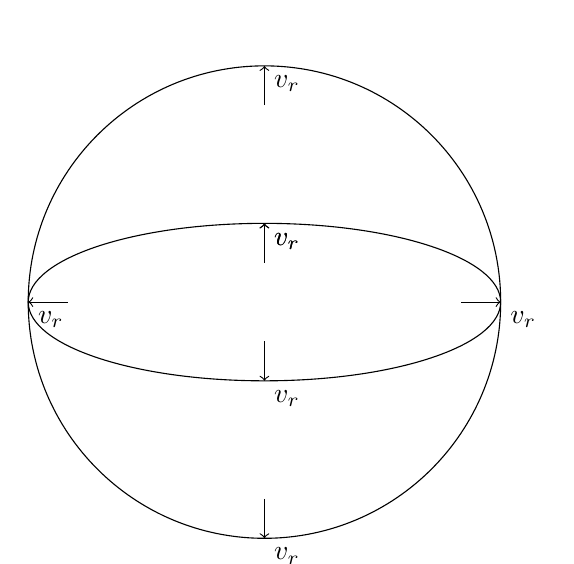
\begin{tikzpicture}
        \draw[->] (0,0.5,0) -- (0,1,0) node[below right] {$v_r$};
        \draw[->] (0,-0.5,0) -- (0,-1,0) node[below right] {$v_r$};
        \draw[->] (0,0.5,0) -- (0,1,0) node[below right] {$v_r$};
        \draw[->] (2.5,0,0) -- (3,0,0) node[below right] {$v_r$};
        \draw[->] (-2.5,0,0) -- (-3,0,0) node[below right] {$v_r$};
        \draw[->] (0,2.5,0) -- (0,3,0) node[below right] {$v_r$};
        \draw[->] (0,-2.5,0) -- (0,-3,0) node[below right] {$v_r$};
        \draw (0,0) circle (3cm);
        \draw (0,0) ellipse (3cm and 1cm);
    \end{tikzpicture}
    \caption{Illustration of a spherical void with radial velocity pointing outwards from the center of the void.}
\end{figure}
The derivation for the radial velocity component is the same for voids as for
filaments up until equation \ref{eq:templineq}. The difference for voids is that
the divergence now has to be calculated in spherical coordinates given by
\begin{equation}
    \nabla\cdot \vec{v}=\frac{1}{r^2}\frac{\partial}{\partial r}(r^2v_r)
                       +\frac{1}{r\mathrm{sin}\theta}\frac{\partial}{\partial r}(\mathrm{sin}\theta v_\theta)
                       +\frac{1}{r\mathrm{sin}\theta}\frac{\partial}{\partial r}(\phi v_\phi).
\end{equation}
As for filaments only the radial component is assumed to be non-negligible
giving
\begin{equation}
    \frac{1}{r^2}\frac{\partial(r^2v_r)}{\partial r}=-Hfa\delta.
\end{equation}
Multiplying by $r^2$ and integrating one will get
\begin{equation}
    v_r = -\frac{1}{r^2}Hfa\int_0^r x^2\delta(x)dx.
\end{equation}
As for filaments a average mass density contrast for voids is defined as
\begin{equation}\label{eq:contrastvoid}
    \Delta_v(r)=\frac{3}{r^3}\int_0^r x^2\delta(x)dx,
\end{equation}
which will give an expression for the radial velocity for voids
\begin{equation}\label{eq:vrvoid}
    v_r(r)=-\frac{1}{3}Hfar\Delta_v(r).
\end{equation}
\subsection{Minor correction term to velocity around voids.}\label{sec:vr_correction}
The equation for the radial velocity around voids given by \ref{eq:vrvoid} is a simple modelling of the velocity using a pure geometrical interpretation. I will implement and test wether adding a correction term to equation \ref{eq:vrvoid} of halos around voids proposed by \cite{Achitouv} will provide better fits to data. The proposed model adds a correctional term to the velocity given as
\begin{equation}\label{eq:achitouv2017}
    v(r)=-\frac{1}{3}Hfar\Delta_v(r)+\Gamma\frac{3}{7}f_2aH\frac{r}{6}\Delta_v^{(2)},
\end{equation}
where $\Gamma=+1$, when $\Delta_v(r)>0$ and $\Gamma=-1$, when $\Delta_v(r)<0$ and i will use $f_2\simeq 2f$ for the sake of my analysis. In addition to the mass density contrast for voids $\Delta_v(r)$ defined in equation \ref{eq:contrastvoid} an additional $\Delta_v^{(2)}$ is introduced as 
\begin{equation}
    \Delta_v^{(2)}(r)\equiv\frac{3}{r^3}\int_0^rx^2\delta(x)^2dx.
\end{equation}
This semi-empirical term is motivated by including a modified second order eularian perturbation term in velocity (eq. (43) in \cite{Catelan_2ndordervelpert})
\begin{equation}
    \nabla\cdot v^{(2)}=\frac{3}{7}f_2aH(\delta^{(1)})^2+\mathrm{Other} \space\mathrm{terms}.
\end{equation}
This modification to the velocity model will be tested by fitting parameters with data when calculating the cross correlation function derived later in section \ref{sec:vgcrosscorr}.
\section{Numerical measurement of correlation functions and multipole expansions.}\label{sec:numerical_corr}
As mentioned in section \ref{sec:corrtheory} correlation functions are useful
tools for measuring the statistical properties of the universe. In order to test
analytical models one has to compare with data from observations or simulations.
The code \footnote{The code for measuring correlation functions utilized for this analysis can be found at \url{https://github.com/seshnadathur/pyCUTE}.} used for this project to measure angular correlation functions
implements a Landy-Szalasay estimator \cite{Landy}. The Landy-Szalasay estimator
for the angular cross correlation function, where $s$ denotes redshiftspace, reads
\begin{equation}
    \xi^s(\vec{s},u)=\frac{\langle D_1D_2\rangle-\langle D_1R_2\rangle-\langle D_2R_1\rangle+\langle R_1R_2\rangle}{\langle R_1R_2\rangle}.
\end{equation}
Where, in this analysis, subscript $1$ denotes either void centers or center or
the center of cosmic filaments and subscript $2$ denotes halo positions. $D_1$
and $D_2$ refers to the actual data while $R$ is samples from a random
distribution resembling the dataset. Each quantity in the squared brackets
denote the mean value of of a pair with separation $r$ and $\mu$, where
$\mu=cos(\theta)$ is the cosine of the angle between the separation vector and
the line of sight direction. An illustration of a pair in the coordinate system
of the observer is illustrated in figure \ref{fig:corrpair}
\begin{figure}\label{fig:corrpair}
    \begin{tikzpicture}
        \def\myrad{2}% radius of the circle
        \def\myang{60}% angle for the arc
        %\draw (0,0) -> (10,0) {s};
        % the origin
        \coordinate (O) at (10,0);
        
        \draw[line width=0.2mm][->] (0,0) -- (10,0);
        \draw[line width=0.2mm][->] (10,0) -- (10-1.414,-1.414);
        \draw[line width=0.2mm][->] (0,0) -- (10-1.414,-1.414);
        % the circle and the dot at the origin
        \node[text width=10cm] at (13.3,0.5) {Filament/void center};
        \node[text width=10] at (5,0.5) {$\vec{r}_{void/filament}$};
        \node[text width=10] at (9.5,-1.4) {$\vec{r}$};
        \node[text width=10] at (5,-1.1) {$\vec{r}_{halo}$};
        \node[text width=5] at (0,1) {Observer};
        \node[text width=5] at (3.7,-1.1*0.34) {$\theta$};
        \draw (O) node[circle] {} circle [radius=\myrad];
        % the ``\theta'' arc
        \draw (O) [thick,domain=330:360] plot ({2+cos(\x)}, {sin(\x)});
    \end{tikzpicture}
    \caption{Figure illustrating the system used in this analysis. This
    figure is drawn in realspace thereby all vectors denoted as $\vec{r}$.
    Transformation to redshiftspace will distort the galaxy positions and the
    corresponding system has vectors denoted as $\vec{s}$.}
\end{figure}
\\\indent
In order to remove the angular dependency, the angular correlation function is
expanded in mulitpoles. The multipoles are given by 
\begin{equation}
    \xi^s_\ell(s)=\int_0^1\xi^s(s,\mu)(1+2\ell)L_\ell(\mu)d\mu
\end{equation}
\cite{Nadathur_corr}, where $L_\ell(\mu)$ are Legendre polynomials
of order $\ell$. In this analysis only the monopole and multipole
are taken into consideration. The Legendre multipoles for $\ell=0$ and
$\ell=1$ are given by
\begin{equation}
    L_0(\mu)=1
\end{equation}
and
\begin{equation}
    L_2(\mu)=(3\mu^2-1)/2.
\end{equation}
\section{Void Analysis}
\subsection{Density profile}\label{sec:voiddensity}
After running the void finding algorithm from REVOLVER on our dataset we have a list of $x$, $y$
and $z$ coordinates for every void center. With a catalogue of void centers one
has to compare their position to the galaxy catalogue in which they are found to
calculate the average density profile as a function of distance from the void
center. Using a periodic kd-tree module \footnote{The periodic kd-tree code
applied for this analysis is found at at \url{https://github.com/patvarilly/periodic_kdtree}} to search for
the nearest halos of the void centers with a gradually increasing radius one can count the halos in
the catalogue close to a given void center. For every void a search for
neghbouring halo particles is conducted with a gradually increasing radius. For
a linearly spaced radius array $\vec{r}=\{r0,\dots,r_{n}\}$ using an iterative
approach every galaxy in a sphere with radius $r_{i}$, where
$i\in\mathbb{N}\bigcap [r_0,r_{n}]$ denotes the
number of iterations, is counted. The total number of halos is stored for
every iteration. For the first iteration the number of halos in a sphere around the void
center is calculated and stored. The density for this sphere is then $n_i/V_i$,
where $n_i$ is the number of halos inside the sphere and $V_i=4\pi r_{i}^3/3$. For
the next iteration the number of halos inside a sphere with radius $r_{i+1}$ is
counted. Alot of the halos inside this new sphere overlaps with the previous
sphere. Therefore the number of halos in the previous step were stored and then
subtracted from the number of galaxies in the new sphere leaving only the number
of halos counted in the spherical shell that does not overlap between the two
spheres. The volume of this spherical shell is $V_{i+1}=4\pi(r_{i+1}^3-r_i^3)/3$. The
number density in the shell defined by subtracting the previous sphere from the
new sphere is the number of galaxies in the new sphere subtracted by the number
of galaxies in the previous sphere divided by the volume of the sperical shell.
The total number of galaxies in the new sphere is stored and this process is
repeat for all iterations defined by the radius vector $\vec{r}$. This process
will give the density profile as a function of radius for a given void. By
adding the density profiles for all voids and diving by the number of voids one
will get an average density profile for the whole dataset.
\subsection{Velocity profile and velocity dispersion}\label{sec:voidvel}
When studying linear theory applied to voids and filaments, one needs an observational or
numerical representation to test its validity. As explained in section
\ref{sec:radlintheory} the radial velocity profile can be represented analytically and
may provide a good comparison. In addition to the $x$, $y$ and $z$ coordinates for the
halo particles, the galaxy catalogue used also containts the $v_x$, $v_y$ and
$v_z$ particles. The radial velocity profile is calculated in a
similar manner as the density profile for voids described in
\ref{sec:voiddensity}. Using a periodic kd-tree centered at the current void one
can count all particles in a sphere around the current void center. For a given
halo particle its position with respect to a given void center is given by
\begin{equation}\label{eq:voidpos}
    \vec{r}=\vec{r}_{\mathrm{void}}-\vec{r}_{\mathrm{halo}}.
\end{equation}
This is the vector that points radially from the void center to a given halo
particle. The radial velocity component is is the component of the velocity of a
given halo particle $\vec{v}$ that points along this vector. The component of vector
$\vec{v}$ along vector $\vec{r}$ is caluclated as
\begin{equation}
    v_r=\frac{\vec{r}\cdot\vec{v}}{\vert\vec{r}\vert}.
\end{equation}
This is the radial velocity for a halo particle with respect to a given void
center. In a similar manner to the density profile the radial velocity is
calculated iteratively for every particle in sphere around the void center. In
order to get the radial velocity profile the particles are divided into
shells. For every iteration, for a given void, for each sphere the radial
velocity is stored for the next iteration. The radial velocity in a given shell
for the next iteration is the radial velocity in the new sphere subtracted by
the radial velocity in the previous sphere. This is averaged by, for each shell,
dividing by the number of particles in a given shell. After this has
been done for all voids the radial velocity profile is divided by the number of voids in the catalogue to get
the average radial velocity profile for a single halo particle in the catalogue.
\\\indent
The velocity dispersion $\sigma_v$ is also calculated. The velocity dispersion
is given by the usual expression for the standard derivation
\begin{equation}\label{eq:sigma_v}
    \sigma_{v} = \sqrt{\langle v^2 \rangle + \langle v\rangle^2}.
\end{equation}
This velocity is along the line of sight for the observer. For the multidark
dataset this is along the $z$ direction and therefore only the $v_z$ component
is considered. This is calculated in spherical shells around each void center to
get the average void velocity dispersion profile.
\subsection{Void-galaxy cross correlation function.}\label{sec:vgcrosscorr}
As mentioned in section \sec{sec:corrtheory} cross correlation functions are
essential tools in cosmology for measuring the statistical properties of
observables in the universe. In this analysis one of the cross correlations that
will be looked into is the cross correlation between void centers and galaxies
or halos. Following the approach of \cite{Nadathur_corr}, the following
subsection will describe how to derive the void-galaxy cross correlation
function. 
\\\indent
Let $\vec{r}_{void}$ denote the position of a void center and $\vec{r}_{halo}$ denote the
position of a halo or galaxy particle in realspace. Their separation vector $\vec{r}$ is then
given by equation \ref{eq:voidpos}. A figure of the system is illustrated in \ref{fig:corrpair}. The relation from redshiftspace to realspace
is given as
\begin{equation}\label{eq:s_to_r}
    \vec{s}=\vec{r}+\frac{\vec{v}_{pec}\cdot\hat{r}_{void}}{aH}\hat{r}_{void},
\end{equation}
where $v_{pec}$ is the peculiar velocity of a galaxy or halo particle and
$\hat{r}_{void}=\vec{r}_{void}/ \vert \vec{r}_{void}\vert$. Here it is assumed
that the velocity of void centers are negligible. The number of voids in
realspace may not be preserved in redshiftspace. Therefore reconstruction,
described here in section \ref{sec:reconstruction}, has to be applied to regain
the field in realspace from redshiftspace if observational data is used.. The basic assumption
required is that the number of void-galaxy pairs in the simulation volume is
unchanged during transformation from realspace to redshiftspace. This is stated
mathematically as
\begin{equation}\label{eq:corr_void_start}
    (1 + \xi^s_{\mathrm{vg}}(\vec{s}))\mathrm{d}^3\mathrm{s}=(1 + \xi^r_{\mathrm{vg}}(\vec{r}))\mathrm{d}^3\mathrm{r},
\end{equation}
where superscript $r$ and $s$ denotes realspace and redshiftspace respectively.
Here $\xi^s_{vg}(\vec{s})$ is the cross correlation between realspace voids and
the redshifted galaxy field and $\xi^r_{vg}(\vec{r})$ is the cross correlation
between realspace voids and realspace galaxy positions. $\vec{r}$ and $\vec{s}$
are vectors pointing from the void center to a given galaxy position in
realspace and redshiftspace respectively. Another assumption made
is that the velocity of all halo particles near a void can be approximated by
its radial velocity $\vec{v}=v_r \hat{r}$. We orient our coordinate system so that
$\hat{r}_{void}=\hat{z}$. The observer will then only experience redshift
distortions in the $z$ direction. This makes $s_x=r_x$ and $s_y=r_y$. With $\hat{r}_{void}=\hat{z}$ then have that
$\hat{r}_{void}\cdot\hat{r}=z/r$. We can then rewrite equation \ref{eq:s_to_r}
as
\begin{equation}
    \vec{s}=\vec{r}+\frac{v_rz}{aHr}\hat{z}.
\end{equation}
The coordinate transformation will then have the
following jacobian determinant
\begin{equation}
    \vert J(\frac{s}{r})\vert=
    \begin{vmatrix}
        1 & 0 & 0\\
        0 & 1 & 0\\
        0 & 0 & \frac{\partial s_z}{\partial r_z} 
    \end{vmatrix},
\end{equation}
where
\begin{equation}
    \frac{\partial s_z}{\partial r_z} = 1 + \frac{v_r}{raH}+\frac{(v_r^\prime-v_r/r)}{aH}\mu^2.
\end{equation}
here $v_r^\prime$ denotes derivative with respect to $r$. One can now rewrite
equation \ref{eq:corr_void_start} as
\begin{equation}\label{eq:corr_temp}
    1 + \xi^s_{\mathrm{vg}}(\vec{s})=(1 + \xi^r_{\mathrm{vg}}(\vec{r})) \Big[1 + \frac{v_r}{raH}+\frac{(v_r^\prime-v_r/r)}{aH}\mu^2 \Big]^{-1}.
\end{equation}
Assuming the dynamics to be accurately modelled in the scope of linear
perturbation theory we have the radial velocity $v_r$ given by equation
\ref{eq:vrvoid}. We also have $\Delta_v^\prime(r)=3(\delta(r)-\Delta_v(r))/r$ giving
\begin{equation}
    v_r^\prime=-Hfa(\delta(r)-\Delta(r)),
\end{equation}
where $\Delta_v(r)$ is the density contrast defined in equation
\ref{eq:contrastvoid}. Inserting this into equation \ref{eq:corr_temp} results
in
\begin{equation}\label{eq:corr_temp2}
    1 + \xi^s_{\mathrm{vg}}(\vec{s})=(1 + \xi^r_{\mathrm{vg}}(\vec{r})) \Big[1 -\frac{f}{3}\Delta(r)-f\mu^2(\delta(r)-\Delta(r))\Big]^{-1}.
\end{equation}
This equation can be expanded using the taylor expansion
$1/(1-x)\approx1+x+\mathcal{O}(x)^2$. When expanding this equation it is
appropriate with a review of the terms. It is
assumed that for voids the density profile is small enough so that terms of
second order in $\delta$ and $\Delta_{v}$ is negligible meaning $\delta^2$,
$\Delta_{v}^2$ and $\delta\Delta_v$ terms are not considered. This leaves us with terms
of order $\delta$ and  $\delta\xi^r$ which proves to give
the model sufficient validity on a range of scales \cite{BeyondBAO}. Equation
\ref{eq:corr_temp2} then reduces to
\begin{equation}\label{eq:corr_no_stream}
    \xi^{s,base}_{\mathrm{vg}}(\vec{s},\mu)=\xi^r(r)+\frac{f}{3}\Delta_v(r)(1+\xi^r(r))+f\mu^2[\delta(r)-\Delta_v(r)](1+\xi^r(r)).
\end{equation}
It is worth noting that since $\xi^r(r)$ is the correlation function in
realspace coordinates, if one is to apply this method to observational data
reconstruction, described in section \ref{sec:reconstruction}, has to be performed. Since observational data is observed in
redshiftspace, one cannot observe $\xi^r(r)$ directly. One therefore has to
perform reconstruction on the data and then perform the correlation function
calculation described in section \ref{sec:numerical_corr} in order to obtain
$\xi^r(r)$. When working with simulation data one has knowledge about the
particle field in redshiftspace and in realspace. However for a test on how the
method performs on observational data it is usefull to perform reconstruction on
the redshifted particle field instead of just using the realspace particle
field.
\\\indent
The correlation function in redshiftspace $\xi^s_{\mathrm{vg}}(\vec{s},\mu)$
relies on the realspace length of the separation vector $\vert\vec{r}\vert$ as
can be seen from equation \ref{eq:corr_no_stream}. The system is illustrated in
figure \ref{fig:corrpair}. For every distance from the void center $s$ in
redshiftspace, we want the corresponding length from the void center $r$ in
realspace to calculate $xi^r_{\mathrm{vg}}(r)$, $\delta(r)$ and $\Delta_v(r)$.
To achieve this we start by decomposing $s$ into a parallel and perpendicual
component using basic trigonometry
\begin{equation}
    s_\parallel=s\mu
\end{equation}
and
\begin{equation}
    s_\perp=s(1-\mu^2).
\end{equation}
In the simulation volume there is only redshiftspace distortions along the line
of sight direction. This will mean that the perpendicual component is unchanged
when changing coordinates from redshiftspace to realspace. The parallel
component is found by the relation
\begin{equation}
    r_\parallel=s_\parallel + s\frac{\beta\delta(s)\mu}{3},
\end{equation}
where $\beta=f/b$.
The correspending realspace separation is then given as
\begin{equation}
    r=\sqrt{r_\parallel^2+r_\perp^2}.
\end{equation}
\subsection{Expanding model to account for velocity dispersion}
The previous model for the void-galaxy correlation function is a good
approximation. However it can be improved by taking into account the velocity
dispersion of galaxies around the void centers in the line of sight direction.
This will provide a more accurate model thereby giving a better fit to data.
Instead of only considering radial velocities another component along the line
of sight direction is added
\begin{equation}
    \vec{v}=v_r\hat{r}+v_\parallel \hat{r}_{void}.
\end{equation}
$v_r$ is the radial velocity used in the previous model given by equation
\ref{eq:vrvoid}. $v_\parallel$ is given by a gaussian probability distribution
$P(v_{\vert\vert})$ with zero mean
\begin{equation}
    P(v_\parallel)=\frac{1}{\sqrt{2\pi}\sigma_{v_{\parallel}}}\mathrm{exp}\Big[-\frac{v_\parallel}{2\sigma_{v_\parallel}^2}\Big].
\end{equation}
Since in our simulation volume we only measure velocities along the line of
sight direction we can take $\sigma_{v_{\parallel}}$ to measured by equation
\ref{eq:sigma_v}. This will give a and integral for calculating the improved
model taking into account dispersion in the velocity of halos \cite{BeyondBAO}
\begin{equation}\label{eq:corr_stream}
    1+\xi^{s,streaming}(s,\mu)=\int_{-\infty}^\infty\frac{1+\xi^{s,base}(s)}{\sqrt{2\pi}\sigma_{v_{\parallel}(r)}}\mathrm{exp}\Big[-\frac{v_\parallel^2}{2\sigma_{v_\parallel}(r)}\Big]dv_\parallel.
\end{equation}
\section{Filament Analysis}
\subsection{Masking the simulation volume}\label{sec:maskingfilament}
When applying the DisPerSE code on the particle distribution the output will be,
for each filament detected, coordinates to the start point of each segment
making up the total filament. For each filament there will be a number of
filament segments with startpoints $\vec{r}_i$. This also makes $\vec{r}_{i+1}$
the endpoint of filament with startpoins $\vec{r}_i$. Each filament segment $F_j$ is
then given by
\begin{equation}
    \vec{F}_{j}=\vec{r}_{i+1}-\vec{r}_i.
\end{equation}
Here $j$ denotes a given filament segment while $i$ denotes the startpoints of the
segments. With this notation $j+1$ is denoted by startpoints $i+2$ and $i+1$ and
so on. When a given filament segment is defined the simulation volume is masked
to remove all particles outside the edges of the start and endpoint of the
filament segment. This is done by defining  two planes perpendicular to
$\vec{F}_j$ with points $\vec{r}_{i+1}$ and $\vec{r}_i$. The equation for a
plane $P$ given a vector $\vec{F}$ and a point $\vec{r}$ is given
by the usual formula
\begin{equation}\label{eq:plane_mask}
    P=F_x(x-r_x)+F_y(y-r_y)+F_z(z-r_z)=0,
\end{equation}
where $x$, $y$ and $z$ are coordinates of the particles in the simulation
volume. In this section this vector will be denoted as $\vec{x}$.
The coordinates $r_x$, $r_y$ and $r_z$ are the components of $\vec{r}$.
For a given filament $F$ segment with startpoint $r_{i}$ and endpoint $r_{i+1}$ the particles kept are the particles
satisfying the following criteria
\begin{equation}
    P_0=F_x(x-r_{i_x})+F_y(y-r_{i_y})+F_z(z-r_{i_z})>0
\end{equation}
and
\begin{equation}
    P_1=F_x(x-r_{{i+1}_x})+F_y(y-r_{{i+1}_y})+F_z(z-r_{{i+1}_z})<0.
\end{equation}
The rest of the particles are masked keeping only the particles in the
simulation volume bound by the two plane parallel to the filament segment
centered in the startpoint and endpoint.

\subsection{Density profile}\label{sec:filamentdensity}
After masking the particle box as described in section \ref{sec:maskingfilament}
we are left with a filament segment $\vec{F}_j$ defined by the start and
endpoints $\vec{r}_{i}$ and $\vec{r}_{i+1}$. The distance each halo particle in
the masked simulation volume to the filament segment is the length of the vector
from the particle perpendicular to the filament axis
\begin{equation}\label{eq:distance_from_filament}
    d=\frac{\vert \vec{x}\times\vec{F}_j\vert}{\vert \vec{F}_j\vert}.
\end{equation}
This will leave us with a catalogue of the closest distance for all particles to
the axis of the filament segment. A histogram is then created of this catalogue
to easily count the number of particles in a given radial distance from the
filament segment. The volume of the spherical shells surrounding the filament segment
containing the particles in the radial bin is then given as
\begin{equation}
    V_i={\pi\vert \vec{F}_j\vert(r_i^2-r_{i-1}^2)}
\end{equation}
where $r_i$ and $r_{i-1}$ denotes the edges of the radial bins for the histogram.
The radial density profile of the filament segment is then given as
\begin{equation}
    \rho_i=\frac{N_i}{V_i},
\end{equation}
where $N_i$ is the number of particles in each radial bin. For each filament segment
this is added together and in the end it is divided by the total number of
filaments to get the average density profile.
\subsection{Velocity profile}
In the galaxy catalogue of halo particles in the simulation volume the $v_x$,
$v_y$ and $v_z$ components of the halo particle velocity $\vec{v}$ is given. To
compare the model from linear theory given in equation \ref{eq:vrfilament} we
need the component perpendicular to the axis of a given filament to get the
radial component. As for the density profile calculation in section
\ref{sec:filamentdensity} let $\vec{F}_j=\vec{r}_{i+1} - \vec{r}_i$ define a given
filament segment. After, for each filament, the particle box is masked as
described in section \ref{sec:maskingfilament}, the radial component
perpendicular to the filament axis is caluclated. The length of the parallel component of the
halo positions $\vec{x}_\parallel$ is calculated as
\begin{equation}
    \vert\vec{x}_\parallel\vert=\sqrt{\vert \vec{x}\vert^2-d^2},
\end{equation}
where $d$ is the distance from the filament given by equation
\ref{eq:distance_from_filament}. The parallel component of the vector $\vec{x}$
is then
\begin{equation}
    \vec{x}_\parallel=\vert\vec{x}_\parallel\vert\frac{\vec{F}_j}{\vert\vec{F}_j\vert}.
\end{equation}
This allows one to easily calculatre the component perpendicular to the filament
axis 
\begin{equation}
    \vec{x}_\perp=\vec{x}-\vec{x}_\parallel.
\end{equation}
To obtain the component of the velocity perpendicular to the filament axis one
has to use the regular formula calculating the component of a vector along
another vector
\begin{equation}
    v_r=\frac{\vec{v}\cdot\vec{x}_\perp}{\vert\vec{x}_\perp\vert}.
\end{equation}
This is calculated for all particles in a given radial bin defined by the
histogram created in the density profile calculation in section
\ref{sec:filamentdensity}. To get the average velocity in each bin, the velocity
in each bin is divided by the number halo particles in each bin. This is then
added to the total velocity profile for each filament. In the end the
velocity is divided by the number of filaments to get the average radial
velocity profile for filaments.
\section{Parametrizing distance scales.}\label{sec:rescale_r}
The fiducial cosmology used will vary from the true cosmology. This will introduce distortions in the distance measurements. As conducted by \cite{BeyondBAO}, the method applied to the analysis in this project wil also parametrize these distortions by introducing two dimensionless ratios. One in the perpendicular and one the parallel direction as
\begin{equation}
    \alpha_\perp=\frac{d_A(z)}{d_A^{\mathrm{fid}}(z)}
\end{equation} 
and
\begin{equation}
    \alpha_\parallel=\frac{H^{\mathrm{fid}}(z)}{H(z)},
\end{equation}
where $d_A$ is the angular diameter distance. The correlation function $\xi^s(\vec{s},\mu)$ is measured using the fiducial
components $s_\parallel^\mathrm{fid}$ and $s_\perp^\mathrm{fid}$. These components are then rescaled using the dimensionless ratios as
\begin{equation}
    s_\parallel=\alpha_\parallel s_\parallel^\mathrm{fid}
\end{equation}
and 
\begin{equation}
    s_\perp = \alpha_\perp s_\perp^\mathrm{fid}.
\end{equation}
Likewise the correlation function in realspace $\xi^r(r)$ takes into account distances in realspace at a given redshift for a fixed cosmology. The corresponding distance in the real universe may vary from this distance and therefore the realspace distance is rescaled as
\begin{equation}\label{eq:r_scaling}
    r=\int_0^1\alpha_\parallel r^{\mathrm{fid}}\sqrt{1+(1+\mu^2)\Big[\frac{\alpha_\perp^2}{\alpha_\parallel^2}-1\Big]}d\mu.
\end{equation}
This rescaling of parameters gives an additional parameter when fitting the models to data as both $\alpha_\perp$ and $\alpha_\parallel$ has to be tested in order to determine the best fit to the distance parametrization. In simulations the fiducial cosmology is known and $\alpha_\parallel=\alpha_\perp=1$. Therefore constraining $\epsilon=\alpha_\perp/\alpha_\parallel$ for a model applied to simulation data can provide a good test of how the model performs.
\subsection{Calibrating dark matter profiles.}\label{sec:dm_calibrate}
When using a linear bias approximation we can simply approximate $\delta(r)_g=\xi_{\mathrm{vg}}^r(r)$ as the realspace correlation function between voids and galaxies and the normalized density profile $\delta(r)$ effectively traces the same quantity. The linear bias approximation itself is to just use $\delta_{\mathrm{dm}}=\delta_\mathrm{g}/b$. However when using a dark matter density profile the bias factor is not considered and instead, in linear theory, $\sigma_8$ is used to scale the amplitude of the density profile. At a given redshift $z$ we then have
\begin{equation}\label{eq:delta_dm_profile}
    \delta(r,z) = \frac{\sigma_8(z)}{\sigma_8^{\mathrm{MD}}}\sigma_8^\mathrm{fid}(r,z),
\end{equation}
where $sigma_8^{\mathrm{MD}}=0.8228$ is the value for $\sigma_8$ for the multidark simulation dataset with $z=1$. For $\sigma_8^\mathrm{fid}(r,z)$, the exact dark matter density profile for the four simulated datasets was not obtained. Instead i will use a dark matter profile for voids obtained from the BigMD mock CMASS galaxy sample described in section (skriv om dette). This dark matter profile will need some extra scaling in order for it to accurately represent the dark matter profile for the dataset used in the this analysis. Its amplitube is scaled by $\sigma_8$ as shown in equation \ref{eq:delta_dm_profile} however beforehand i will scale it using by eye measurement making sure its amplitube is approximately equal to the halo dark matter profile derived from the dataset $\delta_\mathrm{g}(r)$ and dividing by the bias factor for the given dataset. This will make the amplitude roughly in line with what the corresponding dark matter profile for the dataset would have looked like. However the slope may differ. Therefore when scaling the radius an extra $r_\mathrm{scale}$ parameter is multiplied with equation \ref{eq:r_scaling} when scaling the radius for the dark matter density profile. This parameter $r_\mathrm{scale}$ will be included in the likelihood analysis as a part of the model when fitting the data. This will make it so that both the amplitube and the slope of the dark matter density profile will be adjusted when fitting the parameters to the data.
\section{Likelihood analysis.}
In order to test the validity of the models and to see wether the proposed improvements perform better a likelihood analysis is conducted. The likelihood analysis in this thesis largely follows the approach conducted by \cite{BeyondBAO}. The code implementing the Metropolis-hastings MCMC chain is provided by the publicly available Victor code\footnote{The code used for the likelihood analysis is provided by \url{https://github.com/seshnadathur/victor}}. Using the method described in section \ref{sec:numerical_corr} the angular cross correlation function $\xi^s(s,\mu)$ and its multipoles is calculated from a simulated halo catalogue in redshiftspace represented as discrete point particles in. For the purpose of this analysis the Multidark dataset is utilized. (Finn ut hvordan denne referes til og fortel litt mer om den.). The numerical angular cross correlation function  is measured using $80$ linearly spaced bins for $0<\mu<1$ and $30$ linearly spaced bins for $2$Mpc/h$<s<118$Mpc/h. Using the same number of bins and datapoints the corresponding angular cross correlation function in realspace $\xi^r(r)$ is also calculated using the corresponding realspace halo catalogue. Using the methods described in sections \ref{sec:voiddensity} and \ref{sec:voidvel} the density profile and velocity dispersion is calculated for each void in catalogue identified by REVOLVER. The density profile and velocity dispersion is calculated using $30$ linearly spaced bins for $2$Mpc/h$<r<118$Mpc/h. With these quantities calculated one has all the components needed to evaluate equation \ref{eq:corr_stream}.
\subsection{Estimating the covariance matrix}
The covariance matrix used is calculated using patchy mocks provided by the multidark simulation\cite{MDmock1}\cite{MDmock2}. The covariance matrix used is provided together with the code used for the likelihood analysis. A mock catalogue is a galaxy or dark matter halo catalogue is a catalogue that is built from simulations designed to resemble an observed galaxy catalogue. The creation of the covariance matrix used is described in \cite{BeyondBAO}. The covariance matrix is calculated using $1000$ patchy mocks. For each patchy mock the angular cross correlation is measured and expanded into a monopole $\xi_0^s$ and a dipole $\xi_2^s$. The multipoles are then combined into a datavector $\vec{\xi}^s\equiv(\xi_0^s, \xi_2^s)$ for each patchy mock catalogue. The covariance matrix is then calculated as
\begin{equation}
    C=\frac{1}{N-1}\sum_{k=1}^N(\vec{\xi} ^k-\vec{\xi}^k_\mu)(\vec{\xi}^k-\vec{\xi}^k_\mu),
\end{equation} 
where $\vec{\xi}^k_\mu$ is the mean over all the mocks used and $k$ is the index for a given mock.
\subsection{Fitting parameters to data.}
The theory model given by equation \ref{eq:corr_stream} relies on the parameters $\sigma_v$, $\beta=f/b$ through the modelling of $v$ given in section \ref{sec:voidvel} using a linear bias approximation $\delta_\mathrm{dm}=\delta_g/b$, and through the rescaling of $r$ described in section \ref{sec:rescale_r}, it also relies on $\alpha_\perp$ and $\alpha_\parallel$ in which is represented as $\epsilon=\alpha_\perp/\alpha_\parallel$.
Without the linear bias approximation the model relies does not rely on the bias factor $b$ but instead relies on the parameters $\sigma_8$ and $r_\mathrm{scale}$ as described in section \ref{sec:dm_calibrate}. For the linear bias approximation, with and without the added velocity term described in section \sec{sec:vr_correction}, the model then relies on three parameters $(\beta,\sigma_v,\epsilon)$. When using a dark matter profile the parameters needed are the four parameters $(f\sigma_8, \sigma_v, \epsilon, r_\mathrm{scale})$
\\\indent
The victor code utilized for the likelihood analysis implements the approach described by Sellentin \& Heavens \cite{heavens2010statistical} and calculates the $\chi^2$ for each step in the MCMC chain as
\begin{equation}
    \chi^2=(\vec{\xi}^{s,\mathrm{streaming}}-\vec{\xi}^{s})\vec{C}^{-1}(\vec{\xi}^{s,\mathrm{streaming}}-\vec{\xi}^{s})
\end{equation}
and calculate the log-likelihood as
\begin{equation}
    \mathrm{ln}\mathcal{L}\propto-\frac{N}{2}\mathrm{ln}\big(1+\frac{\chi^2}{N-1}\big),
\end{equation}
where $N$ is the number of mocks used to calculate the covariance matrix. In this case we have $N=1000$.
\chapter{Results/Discussion}\label{sec:results}
The following section is split into two sections. One section is devoted to the analysis conducted on filaments and another section to the analysis conducted on voids. Throughout this analysis, a fiducial cosmology is assumed. Every time a quantity relying on cosmological parameter is illustrated, the following values were used: $H_0=100h$kms$^{-1}$Mpc$^{-1}$, $\Omega_m=0.31$ and $\Omega_\Lambda=0.69$. 
\section{Filament analysis}\label{sec:filaments}

\subsection{Effect of choosing persistence ratio on dataset}
As discussed in section \ref{sec:persistence}, DisPerSE has an option to filter
noise through setting a persistence threshold. This has a profound effect on the number of filaments identified. Figures \ref{fig:scatterMD1} and \ref{fig:scatterMD2} shows a slice of the MD1 and MD2 datasets. In these figures, filaments identified by DisPerSE are overplotted. The sigma thresholds ranges from no cuts, $\sigma=1$, $\sigma=2$ and $\sigma=3$. From these figures, one can see that increasing the $\sigma$ threshold will reduce the number of filaments detected. Figures \ref{fig:histMD1} and \ref{fig:histMD2} shows histograms of the filament lengths for all filaments in the MD1 and MD2 datasets with the different $\sigma$ thresholds. From the histograms, one can clearly see that filaments with lengths in the range $20$Mpc/h to $50$Mpc/h are the ones that get significantly reduced as the $\sigma$ threshold increases. By looking at the scatter plots for the two datasets, one can see that with no cuts, a lot of knots appear in the intersection where filaments meet. This leads to many individual structures identified as filaments that, in reality, should only make up one individual filament. On the other hand, using $\sigma=3$, leaves out a lot of structures that should be interpreted as filaments. Therefore, the following analysis will be conducted using the filament catalogues output by disperse using $\sigma=1$ and $\sigma=2$. Looking at the histograms, a lot of very large filaments with length $l\geq 100$ is also detected. Although the code is utilized on a dark matter halo catalogue and not a galaxy catalogue, which in principle could make us detect larger structures, filaments with length larger than $100$ Mpc/h is neglected. Although very large structures, such as the Hercules-Corona Borealis Great Wall, in which is approximated to measure around $2000-3000$Mpc in diameter \cite{herculescorona}, exists, to not account for structures larger than what breaks with the cosmological principle, the largest filaments are cut from the catalogue. To avoid small filaments making up potential knots in the intersection where many filaments meet, filaments with length $l\leq 20$Mpc/h are also cut from the catalogue.
\begin{figure}[H]
    \subfigure[]{\includegraphics[width=0.5\textwidth]{figures/scatterplots/scatter_MD1_all.pdf}}\hspace{1em}%
    \subfigure[]{\includegraphics[width=0.5\textwidth]{figures/scatterplots/scatter_MD1_s1.pdf}}
    \subfigure[]{\includegraphics[width=0.5\textwidth]{figures/scatterplots/scatter_MD1_s2.pdf}}\hspace{1em}%
    \subfigure[]{\includegraphics[width=0.5\textwidth]{figures/scatterplots/scatter_MD1_s3.pdf}}
    \caption{Figure showing a slice of the MD1 dataset for $950$Mpc/h$\leq z\leq1050$Mpc/h in the $x$, $y$ plane. Here the persistance threshold given to DisPerSE is varied between no cuts (a), $\sigma=1$ (b), $\sigma=2$ (c), $\sigma=3$ (d).}
    \label{fig:scatterMD1}
\end{figure}
\begin{figure}[H]
    \subfigure[]{\includegraphics[width=0.5\textwidth]{figures/scatterplots/scatter_MD2_all.pdf}}\hspace{2em}%
    \subfigure[]{\includegraphics[width=0.5\textwidth]{figures/scatterplots/scatter_MD2_s1.pdf}}
    \subfigure[]{\includegraphics[width=0.5\textwidth]{figures/scatterplots/scatter_MD2_s2.pdf}}\hspace{2em}%
    \subfigure[]{\includegraphics[width=0.5\textwidth]{figures/scatterplots/scatter_MD2_s3.pdf}}
    \caption{Figure showing a slice of the MD2 dataset for $975$Mpc/h $\leq z\leq1025$Mpc/h in the $x$, $y$ plane. Here the persistance threshold given to DisPerSE is varied between no cuts (a), $\sigma=1$ (b), $\sigma=2$ (c), $\sigma=3$ (d). Each blue dot represents a halo particle while all lines represents filaments assigned by DisPerSE.}
    \label{fig:scatterMD2}
\end{figure}

\begin{figure}[H]
    \subfigure[]{\includegraphics[width=0.5\textwidth]{figures/histograms/filament_histMD1_all.pdf}}\hspace{1em}%
    \subfigure[]{\includegraphics[width=0.5\textwidth]{figures/histograms/filament_histMD1_s1.pdf}}
    \subfigure[]{\includegraphics[width=0.5\textwidth]{figures/histograms/filament_histMD1_s2.pdf}}\hspace{1em}%
    \subfigure[]{\includegraphics[width=0.5\textwidth]{figures/histograms/filament_histMD1_s3.pdf}}
    \caption{Figure showing histograms of filament lengths calculated by disperse the MD1 dataset. Here the persistance threshold given to DisPerSE is varied between no cuts (a), $\sigma=1$ (b), $\sigma=2$ (c), $\sigma=3$ (d). Each blue dot represents a halo particle while all lines represents filaments assigned by DisPerSE.}
    \label{fig:histMD1}
\end{figure}

\begin{figure}[H]
    \subfigure[]{\includegraphics[width=0.5\textwidth]{figures/histograms/filament_histMD2_all.pdf}}\hspace{2em}%
    \subfigure[]{\includegraphics[width=0.5\textwidth]{figures/histograms/filament_histMD2_s1.pdf}}
    \subfigure[]{\includegraphics[width=0.5\textwidth]{figures/histograms/filament_histMD2_s2.pdf}}\hspace{2em}%
    \subfigure[]{\includegraphics[width=0.5\textwidth]{figures/histograms/filament_histMD2_s3.pdf}}
    \caption{Figure showing histograms of filament lengths calculated by disperse the MD2 dataset. Here the persistance threshold given to DisPerSE is varied between no cuts (a), $\sigma=1$ (b), $\sigma=2$ (c), $\sigma=3$ (d).}
    \label{fig:histMD2}
\end{figure}
\subsection{Density profiles}\label{sec:filamentdensityres}
In accordance with the method described in section \ref{sec:filamentdensity}, the density profile $\rho_g(r)/\bar{\rho}$ was calculated for the MD1 and MD2 datasets with $\sigma=1$ and $\sigma=2$ as inputs to the DisPerSE code. The density profile was calculated from $r=0$Mpc/h to $r=300$Mpc/h using linearly spaced bins of size $2$Mpc/h. This is a very long distance, but in order to test the scales at which linear theory could be applied to filaments, an arbitrarily large distance was chosen. From the histogram of filament lengths, illustrated in figures \ref{fig:histMD1} and \ref{fig:histMD2}, one can see that increasing the $\sigma$ threshold for the DisPerSE code greatly reduces the amount of shorter filaments. From the MD1 one dataset for both $\sigma$-thresholds chosen, illustrated in figures \ref{fig:fildensitytMD1s1} and \ref{fig:fildensitytMD1s2}, one can see that the density close to the filament spine is larger for the higher $\sigma$-threshold. This is also present for the MD2 dataset, as shown when comparing figures \ref{fig:fildensitytMD2s1} and \ref{fig:fildensitytMD2s2}. As one could see from the histograms of filaments, increasing the $\sigma$-threshold reduced the number of smaller filaments. This may suggest that longer filaments possess a higher number density of particles per volume. This result may also be an effect of noise removed when cutting shorter filaments as the shorter filaments, represented in the lower $\sigma$-threshold, may be structures identified in more sparse areas of the simulation volume thereby lowering the stacked density profile.\\\indent
As can be seen from the figures of the density profiles, a power law model was fitted to the density profile from the filament spine to approximately where the profile reaches the average density of the simulation volume. For the MD1 dataset the density profile flattens out at approximately $r=30$Mpc/h for both $\sigma$-thresholds. For the MD2 dataset this happens at roughly $r=20$Mpc/h for both $\sigma$-thresholds. This distance is longer than what is detected by \cite{Gal_rraga_Espinosa_2020} (e.g fig.9). Using a similar method applied to the TNG300 simulation\cite{nelson2021illustristng} at redshift $z=0$, they found that the density profile converged to the average density of the simulation volume at approximately $r=7$Mpc/h-$21$Mpc/g depending on dataset and length cuts applied to filaments. They also found that long filaments converged faster than shorter filaments. A similar method was also applied by \cite{bonjean} (e.g fig.5) to galaxies in the range $0.1<z<0.3$ using the WISExSCOS catalogue\cite{Bilicki_2016}. They calculated the stacked overdensity profile and their results shows that the gradient flattens out at approximately $21$Mpc/h. The calculations in this thesis on the other hand is conducted at $z=1$. For both datasets and $\sigma$-thresholds a power law $\propto r^x$ was fitted using the density profiles from $r=0$Mpc/h to $r=30$Mpc/h for the MD1 dataset and $r=0$Mpc/h to $r=20$Mpc/h for the MD2 dataset. These results suggests that there is a steeper gradient when increasing the $\sigma$ threshold. This may suggest that longer filaments are more dense or it may simply be an artifact of DisPerSE removing shorter filaments that should be percieved as noise. In order to test this, it would be useful for future expansion of these results to test the algorithm on filaments of different lengths by applying manual cuts to the filament catalogue using the same $\sigma$-threshold.\\\indent
After the density profiles reaches the average density of the simulation volume, for the two sigma thresholds in the MD1 dataset, there is a prominent bulge which peaks at approximately $r=100$Mpc/h. For the density profiles derived from the MD2 dataset this is bulge is not as prominent, but after approximately $r=60$Mpc/h, the density profile starts to decline slowly. This effect may be due to a potential artifact where the volume of the cylindrical shells surrounding the filament does not scale properly with the amount of halos counted in each shell. However, the prominent bulge in the MD1 dataset may instead suggest that this may instead be a feature of the dataset itself. The MD2 dataset, in which is a lot more dense seems to wash out this bulge as it is not as prominent in this dataset. There is also a prominent difference in that, when choosing $\sigma=1$ or $\sigma=2$ as input to DisPerSE, the level at which the gradient flattens out relative to the background density changes slightly. This however may be due to increasing $\sigma$-threshold effectively lowers the amount of shorter filaments which, again, may suggest that longer filament are more dense. It may also be an effect of DisPerSE correctly rooting out filaments that should be percieved as noise when increasing $\sigma$-threshold. The apparent bulge in the MD1 dataset may make this density profile problematic when applying it to linear theory to calculate the velocity, given in equation \ref{eq:vrfilament}. However, the density profiles for the MD2 dataset should be sufficient on scales up to $r=60$Mpc/h.
\begin{figure}[H]
    \includegraphics{figures/Density_profiles/Filaments/delta_MD1_s1.pdf}
    \caption{Figure showing the calculated density profile $\rho_g(r)/\bar{\rho}$ for filaments in the MD1 dataset with $\sigma=1$.}
    \label{fig:fildensitytMD1s1}
\end{figure}

\begin{figure}[H]
    \includegraphics{figures/Density_profiles/Filaments/delta_MD1_s2.pdf}
    \caption{Figure showing the calculated density profile $\rho_g(r)/\bar{\rho}$ for filaments in the MD1 dataset with $\sigma=2$.}
    \label{fig:fildensitytMD1s2}
\end{figure}

\begin{figure}[H]
    \includegraphics{figures/Density_profiles/Filaments/delta_MD2_s1.pdf}
    \caption{Figure showing the calculated density profile $\rho_g(r)/\bar{\rho}$ for filaments in the MD2 dataset with $\sigma=1$.}
    \label{fig:fildensitytMD2s1}
\end{figure}

\begin{figure}[H]
    \includegraphics{figures/Density_profiles/Filaments/delta_MD2_s2.pdf}
    \caption{Figure showing the calculated density profile $\rho_g(r)/\bar{\rho}$ for filaments in the MD2 dataset with $\sigma=2$.}
    \label{fig:fildensitytMD2s2}
\end{figure}
\subsection{Radial velocity profiles}
In order to test wether linear theory could be used to approximate the behavior halos around filaments, the theory, described in section \ref{sec:filamentvr}, was applied using the density profiles shown in section \ref{sec:filamentdensityres}. The velocity profile, calculated numerically from the dataset, was calculated from $r=0$Mpc/h to $r=300$Mpc/h using linearly spaced bins of size $2$Mpc/h. Figures \ref{fig:filvrMD1s1} and \ref{fig:filvrMD1s2} shows the velocity of filaments predicted by linear theory compared with the velocity calculated from the dataset, as described in section \ref{sec:numfilamentvelocity}, for the MD1 dataset with $\sigma=1$ and $\sigma=2$ respectively. Figures \ref{fig:filvrMD2s1} and \ref{fig:filvrMD2s2} shows the same for the MD2 dataset. As can be seen from the figures of the density profiles in the previous section, the density profiles did not have a gradient that was approximately zero after it flattened out and reached the average density of the simulation volume. Instead, it showed a slow decline for the MD2 dataset and a more prominent bulge for the MD1 dataset. The small negative gradient in the density profile, from equation \ref{eq:vrfilament}, causes the velocity predicted by linear theory to have an artificial increase on large scales. In order to counteract this, the overdensity $\delta_g(r)=\rho_g(r)/\bar{\rho}-1$ was artificially set to zero for scales $r>50$Mpc/h. For all datasets the numerically calculated velocity has a radial component with a relatively large value close to the filament spine before it declines and eventually reaches zero. This is reasonable as far away from the filament spine, the stacked velocity profile should not be biased in any direction. All the velocity profiles display a feature in which appears as a hook close to the filament spine. This may be due to the halos being inside the densest parts of the filament experience a greater gravitational attraction from multiple sides making the net acceleration towards the filament spine smaller. Another explanation for this effect may be that one could imagine the densest parts of the filaments being at the edges of the filaments in large clusters. Overdensities at the end points of the filament spine will make matter flow along the vector parallel to the spine itself, thereby decreasing the amplitude of the radial component. Studying the two-dimensional velocity field around filaments may be of interest in order to verify wether this could be a reasonable explanation. From the figures, it is also evident that the measured velocity profiles flattens out and starts to converge towards the background density of the simulation volume on scales $r>100$Mpc/h \\\indent
The velocities predicted by linear theory displays the same behavior as the velocity measured from the catalogues themselves. Their amplitude however is much larger than what should be expected as measured from the dataset. As expected there is also a prominent bend on the velocity profile predicted by linear theory at $r=50$, where $\delta_g(r)$ was set to zero. Since one has the simulation to compare with, one could use eye measurements to move the radius at which one sets $\delta_g(r)=0$. However if this was to be used for observational data, one is not able to make this comparison, and therefore, this limit was set at $r=50$Mpc/h. As can be seen from the density profiles from the previous section, choosing $\sigma=2$, made the measured density at the center of the filament larger. This is also evident in that the velocity profiles predicted by linear theory has a higher amplitude for $\sigma=2$ relative to $\sigma=1$ close to the filament spine. Although the density profiles using $\sigma=2$ gave more reasonable results for large radii, since $\delta(r>50$Mpc/h$)$ is set to zero, this potential effect on predicted velocity profile is not evident in these results. These results however, show that linear theory can be used to predict the shape of radial velocity profile. However, more effort should to be put into studying the amplitude. Since the predicted velocity profile is directly dependent on the density profile, it may be worth investing effort into studying how the methodology for calculating the density profile can be improved. 


\begin{figure}[H]
    \includegraphics{figures/Theory_vs_v_r/Filaments/vr_MD1_s1.pdf}
    \caption{Figure showing the calculated radial velocity profile compared with the predictions from linear theory for filaments in the MD1 dataset with $\sigma=1$.}
    \label{fig:filvrMD1s1}
\end{figure}

\begin{figure}[H]
    \includegraphics{figures/Theory_vs_v_r/Filaments/vr_MD1_s2.pdf}
    \caption{Figure showing the calculated radial velocity profile compared with the predictions from linear theory for filaments in the MD1 dataset with $\sigma=2$.}
    \label{fig:filvrMD1s2}
\end{figure}

\begin{figure}[H]
    \includegraphics{figures/Theory_vs_v_r/Filaments/vr_MD2_s1.pdf}
    \caption{Figure showing the calculated radial velocity profile compared with the predictions from linear theory for filaments in the MD2 dataset with $\sigma=2$.}
    \label{fig:filvrMD2s1}
\end{figure}

\begin{figure}[H]
    \includegraphics{figures/Theory_vs_v_r/Filaments/vr_MD2_s2.pdf}
    \caption{Figure showing the calculated radial velocity profile compared with the predictions from linear theory for filaments in the MD2 dataset with $\sigma=2$.}
    \label{fig:filvrMD2s2}
\end{figure}
\section{Void analysis}\label{sec:void}
\subsection{Histograms}
The effective void radius, measured in Mpc/h, is one of the quantities of voids that is derived from the void finder in the REVOLVER code. Figures \ref{fig:voidhistMD2}, \ref{fig:voidhistMD2} and \ref{fig:voidhistMD4} shows histograms of the effective void radius found in the MD2, MD3 and MD4 datasets respectively. The histograms were calculated using radial bins with a size of $2$Mpc/h. Due to a small sample size, giving lots of noise and bad fits to the cross correlation function, the MD1 dataset was excluded from the void analysis. From the figures, one can see that for the MD2 and MD3 datasets, the bulk of the distribution of voids is in the $20$Mpc/h to $80$Mpc/h range. With the MD4 dataset the distribution is tilted more towards smaller voids with the peak of the distribution at approximately $30$Mpc/h. This trend can be seen throughout all the three datasets tested. The more halo particles in the catalogue, the more the distribution shifts towards smaller voids. This is a reasonable result as a catalogue that is highly populated will introduce more irregularities to the density field from which the voids are defined than a more sparsely populated catalogue. The amount of small voids however can introduce physical effects that may not be accurately approximated by linear theory. If the voids are small enough, non-linear interactions between halo particles may start to dominate. This can make the assumptions from section \ref{sec:radlintheory}, such as the velocity of halos being purely in the radial direction, prove to not be a good approximation for their real behavior. Therefore, in order study wether this is the case, the MD3 and MD4 datasets was split into three different cuts. One catalogue containing all voids, one catalogue containing small voids with effective radius $20$Mpc/h$\leq 40$Mpc and one catalogue with large voids containing voids with $r\geq 40$Mpc/h. 

\begin{figure}[H]
    \includegraphics{figures/histograms/void_histogramMD2.pdf}
    \caption{Figure showing a histogram of the effective void radius of voids found in the Multidark 2 dataset.}
    \label{fig:voidhistMD2}
\end{figure}
\begin{figure}[H]
    \includegraphics{figures/histograms/void_histogramMD3.pdf}
    \caption{Figure showing a histogram of the effective void radius of voids found in the Multidark 3 dataset.}
    \label{fig:voidhistMD3}
\end{figure}
\begin{figure}[H]
    \includegraphics{figures/histograms/void_histogramMD4.pdf}
    \caption{Figure showing a histogram of the effective void radius of voids found in the Multidark 4 dataset.}
    \label{fig:voidhistMD4}
\end{figure}
\subsection{Density profiles}
In accordance with the method described in section \ref{sec:voiddensity}, the density profiles of voids $\delta(r)$ were calculated. The density profile was calculated for $2$Mpc/h$\leq r\leq 118$Mpc/h and then splined using linear interpolation. The density profile for voids found in the MD2 dataset is illustrated in figure \ref{fig:deltaMD2}. The density profiles for the MD3 and MD4 with and without cuts, where only voids with radius radius $20$Mpc/h$\leq r\leq 40$Mpc/h and $r\geq 40$ Mpc/h are included, is shown in figures \ref{fig:deltadmMD3} and \ref{fig:deltadmMD4} respectively. From these figures one can see that in the void center the density is zero. As the radius increase, the overdensity profile starts to increase before it reaches a maximum value. This is due to the fact that overdensities are usually found on the edges of voids as matter flows away from underdensities found in the center of the void itself. After the profile reaches is maximum, the density profile declines and far away from the void center, the average density profile converges towards the average density of the simlation volume. One can see from these figures that applying cuts will shift the peak of the overdensity. Larger voids will peak at a larger radius than the smaller voids. The smaller voids also has a more prominent overdensity than the larger voids.\\\indent
 

\begin{figure}[H]
    \includegraphics{figures/Density_profiles/Voids/density_profileMD2.pdf}
    \caption{Figure showing the density profile for voids found in the Multidark 2 dataset.}
    \label{fig:deltaMD2}
\end{figure}
\begin{figure}[H]
    \includegraphics[width=1\textwidth]{figures/Density_profiles/Voids/density_profileMD3.pdf}
    \caption{Figure showing the density profile for voids found in the Multidark 3 dataset. Here the radius of voids considered are in the radius range of: all voids: top figure, $20$Mpc/h $\leq r\leq 40$Mpc/h in the bottom left, and $r\geq 40$Mpc/h in the bottom right.}
    \label{fig:deltaMD3}
\end{figure}
\begin{figure}[H]
    \includegraphics[width=1\textwidth]{figures/Density_profiles/Voids/density_profileMD4.pdf}
    \caption{Figure showing the density profile for voids found in the Multidark 4 dataset. Here the radius of voids considered are in the radius range of: all voids: top figure, $20$Mpc/h $\leq r\leq 40$Mpc/h in the bottom left, and $r\geq 40$Mpc/h in the bottom right.}
    \label{fig:deltaMD4}
\end{figure}
These density profiles was also used to calibrate the dark matter density profile as described in section \ref{sec:dm_calibrate}. This is shown in figures \ref{fig:deltadmMD2}, \ref{fig:deltadmMD3} and \ref{fig:deltadmMD4} for the three datasets tested.
In these figures, the blue lines labeled "Scaled $\delta_{dm}(r)$" is the dark matter profile multiplied by a scaling factor in order for the amplitube to resemble that of $\delta_g(r)$. This factor was set to $1.85$. For use in the model for the correlation function, after it was scaled with the $1.85$ factor, the dark matter profile was divided by the bias term for the given MultiDark dataset it was utilized on. The bias factor for each dataset is listed in table \ref{tab:MDproperties}. This is illustrated by the orange line.
The dark matter density profile is not as steep as the dark matter halo profile. This is because as $\delta_g(r)$ traces a discrete particle field, $\delta_{dm}(r)$ resembles a more fluid like behavior. Although, in this work, the real dark matter profile for the dataset was not obtained and instead a dark matter profile from another dataset was utilized, the principle for this behavior is the same. The catalogue used to calculate $\delta_{dm}(r)$ is found from the dark matter particle field and is a point particle distribution derived from a much larger amount of dark matter particles. The Larger amount of particles in the dark matter particle field will even out the slope of the density profile.\\\indent 
\begin{figure}[H]
    \includegraphics{figures/Density_profiles/Voids/DM_profile_MD2.pdf}
    \caption{Figure showing the calibrated dark matter density profile, in accordance with the method described in section \ref{sec:dm_calibrate}, for voids found in the Multidark 2 dataset. The blue line is the dark matter density profile multiplied by a factor $1.85$ in order to make it resemble $\delta_g(r)$. The orange line is the scaled dark matter density profile divided by the bias factor for the given MultiDark dataset. The orange line is the one used in the calculation of the model.}
    \label{fig:deltadmMD2}
\end{figure}

\begin{figure}[H]
    \includegraphics{figures/Density_profiles/Voids/DM_profile_MD3.pdf}
    \caption{Figure showing the calibrated dark matter density profile, in accordance with the method described in section \ref{sec:dm_calibrate}, for voids found in the Multidark 3 dataset. The blue line is the dark matter density profile multiplied by a factor $1.85$ in order to make it resemble $\delta_g(r)$. The orange line is the scaled dark matter density profile divided by the bias factor for the given MultiDark dataset. The orange line is the one used in the calculation of the model.}
    \label{fig:deltadmMD3}
\end{figure}

\begin{figure}[H]
    \includegraphics{figures/Density_profiles/Voids/DM_profile_MD4.pdf}
    \caption{Figure showing the calibrated dark matter density profile, in accordance with the method described in section \ref{sec:dm_calibrate}, for voids found in the Multidark 4 dataset. The blue line is the dark matter density profile multiplied by a factor $1.85$ in order to make it resemble $\delta_g(r)$. The orange line is the scaled dark matter density profile divided by the bias factor for the given MultiDark dataset. The orange line is the one used in the calculation of the model.}
    \label{fig:deltadmMD4}
\end{figure}
In order to calculate the correlation function given in equations \ref{eq:corr_no_stream} and \ref{eq:corr_stream}, the density contrast for voids $\Delta_v(r)$, given in equation \ref{eq:contrastvoid}, was calculated for all the datasets with the aforementioned cuts. This is illustrated in the figures \ref{fig:DeltaMD2}, \ref{fig:DeltaMD3} and \ref{fig:DeltaMD4}. 
\begin{figure}[H]
    \includegraphics{figures/Density_profiles/Voids/DeltaMD2.pdf}
    \caption{Figure showing the density contrast $\Delta_v(r)$ for voids found in the Multidark 2 dataset.}
    \label{fig:DeltaMD2}
\end{figure}
\begin{figure}[H]
    \includegraphics[width=1\textwidth]{figures/Density_profiles/Voids/DeltaMD3.pdf}
    \caption{Figure showing the density contrast $\Delta_v(r)$ for voids found in the Multidark 3 dataset. Here the radius of voids considered are in the radius range of: all voids: top figure, $20$Mpc/h $\leq r\leq 40$Mpc/h in the bottom left, and $r\geq 40$Mpc/h in the bottom right.}
    \label{fig:DeltaMD3}
\end{figure}
\begin{figure}[H]
    \includegraphics[width=1\textwidth]{figures/Density_profiles/Voids/DeltaMD4.pdf}
    \caption{Figure showing the density contrast $\Delta_v(r)$ for voids found in the Multidark 4 dataset. Here the radius of voids considered are in the radius range of: all voids: top figure, $20$Mpc/h $\leq r\leq 40$Mpc/h in the bottom left, and $r\geq 40$Mpc/h in the bottom right.}
    \label{fig:DeltaMD4}
\end{figure}

\subsection{Radial velocity profiles}
The radial velocity profile $v_r(r)$ for all three datasets was calculated in accordance with the method described in section \ref{sec:voidvel}. The numerically calculated velocity profile was calculated for $2$Mpc/h$\leq r\leq 118$Mpc/h using $30$ linearly space bins. After this, the radial velocity profile $v_r(r)$ was splined using linear interpolation. These were also compared with the predicted radial velocity from linear theory, given in equation \ref{eq:vrvoid}. This is illustrated in figures \ref{fig:vrMD2}, \ref{fig:vrMD3} and \ref{fig:vrMD4} for the MD2, MD3 and MD4 datasets respectively. From these figures, one can see that the measured radial velocity is in the range of approximately $150$km/s. This velocity is similar to what is measured in \cite{Nadathur_2018} (e.g, figure 2) and \cite{Achitouv_streaming} (e.g, figure 2). The radial velocity is zero close to the center of the void as these areas are empty of halos. The stacked radial velocity then starts to increase. Positive direction is pointing radially inwards towards the void center, and therefore, the velocity increases in the negative direction as matter is drawn outwards, flowing towards overdensities at the edges of voids. After the radial velocity reaches its maximum, it declines and reaches zero as other dynamics than that of the void itself starts to dominate. On these radii, the radial velocity is no longer biased along the radial vector of the void making the stacked radial velocity profile zero. From the figures for the radial velocity, one can see that when applying cuts, there is a significant increase in velocity for the stacked velocity profile. \\\indent
A qualitative comparison shows that the radial velocity predicted by linear theory matches the numerically calculated reasonably well on scales approximately $r>30$Mpc/h. However, on smaller radii, it is evident that the predicted velocity does not capture the behaviour the numerically calculated velocity. The numerically calculated velocity has a zero gradient on small scales closer to the void center. However, the velocity predicted by linear theory starts with a steep gradient. For the datasets without cuts, one can see that this will result in the peak of the stacked velocity occuring earlier than that of the numerically calculated velocity. However, when the $r>40$Mpc/h cut is applied for the MD3 and MD4 datasets, both the amplitude and peak of the curve predicted by linear theory coincides with the numerically calculated a lot closer. After the velocity starts to decline, for the $r>40$Mpc/h cut, the numerical and predicted curve match each other in an almost identical fashion. When no cuts are applied, and for the $20$Mpc/h$<r<40$Mpc/h cuts, there is a slight offset between the two curves. This suggests that linear theory is a good approximation to the radial velocity for voids when cuts are applied, and small voids subject to non-linear dynamics are left out of the catalogue.\\\indent
The predicted radial velocity with the correction term, given in equation \ref{eq:achitouv2017}, was also calculated. For the MD2, and the MD3 and MD4 datasets without cuts, this model has an amplitude that is more in line with the numerical calculation. This is in agreement with what the author of \cite{Achitouv_streaming} found when implementing this model. On lower radii, before the stacked velocity reaches its maximum, the model with the correction term seems to be in better agreement with the data found from the catalogue. However, he author found this model to perform better than the regular velocity proposed by linear theory on all scales. This is in contrast to what is suggested from the results found here for these datasets. On larger scales, when the numerical curve decreases, the regular predictions from linear theory seem to be in better agreement. It is worth noting that for all three samples without cuts and the samples with the $20$Mpc/h$<r<40$Mpc/h cuts, there is a discontinuity in the velocity predicted by the model with the correction term. This discontinuity stems from the $\Gamma$ factor in equation \ref{eq:achitouv2017}. When the $\Delta_v(r)$ changes from negative to positive, the $\Gamma$ factor changes from $-1$ to $+1$. This gives rise to the discontinuity observed in the velocity predicted by this model. This discontinuity makes the model appear better than the regular linear theory model on larger radii. For the MD3 and MD4 datasets with the $r>40$Mpc/h cuts applied, there is a better agreement on the amplitude between the numerical data and the regular velocity predicted by linear theory. On these datasets, with the given cuts, the model with the correction term underestimates the peak of the velocity. On larger radii there is a good agreement between the numerically calculated model and the velocity predicted by linear theory using these cuts. For the model with the correction term however there is a small discrepancy on these scales. Overall, these results suggest that the model predicted by linear theory is a better predictor for the velocity of halos around voids when cuts excluding small voids are applied. The model with the correction term, on the other hand, seem to model the smaller voids better, as is evident in the amplitude having a better agreement. It is therefore not clear if there is a significant difference between the models with these cuts when doing a pure qualitative comparison.
\begin{figure}[H]
    \includegraphics[width=1\textwidth]{figures/Theory_vs_v_r/Voids/vr_comparison_MD2.pdf}
    \caption{Figure showing the radial velocity profile halos around voids found in the Multidark 2 dataset. Here it is compared with the prediction from linear theory given in equation \ref{eq:vrvoid}.}
    \label{fig:vrMD2}
\end{figure}

\begin{figure}[H]
    \includegraphics[width=1\textwidth]{figures/Theory_vs_v_r/Voids/vr_comparisonMD3.pdf}
    \caption{Figure showing the radial velocity profile halos around voids found in the Multidark 3 dataset. Here it is compared with the prediction from linear theory given in equation \ref{eq:vrvoid}. Here the radius of voids considered are in the radius range of: all voids: top figure, $20$Mpc/h $\leq r\leq 40$Mpc/h in the bottom left, and $r\geq 40$Mpc/h in the bottom right.}
    \label{fig:vrMD3}
\end{figure}

\begin{figure}[H]
    \includegraphics[width=1\textwidth]{figures/Theory_vs_v_r/Voids/vr_comparisonMD4.pdf}
    \caption{Figure showing the radial velocity profile halos around voids found in the Multidark 4 dataset. Here it is compared with the prediction from linear theory given in equation \ref{eq:vrvoid}. Here the radius of voids considered are in the radius range of: all voids: top figure, $20$Mpc/h $\leq r\leq 40$Mpc/h in the bottom left, and $r\geq 40$Mpc/h in the bottom right.}
    \label{fig:vrMD4}
\end{figure}
The last major component entering the correlation function in equation \ref{eq:corr_stream} is the velocity dispersion $\sigma_{v_z}$. The velocity dispersion was calculated for $2$Mpc/h$\leq r\leq 118$Mpc/h using $30$ linearly space bins and was then splined using linear interpolation. This quantity was calculated for all three datasets with and without the aforementioned cuts and is illustrated in figures \ref{fig:sigmavMD2}, \ref{fig:sigmavMD3} and \ref{fig:sigmavMD4} for the three datasets respectively. As in \cite{Nadathur_corr} and \cite{Achitouv_streaming}, the velocity dispersion profile converges to a value of around $300-350$ km/s, giving good agreement with previous works. However, close to the void center the dispersion profile is noisy. If few of the voids contains halo particles close to the void center, they will be accounted for, and since the method divides by the amount of particles in a given radial bin around the void, bins with small number of particles can provide an unproportionately large contribution. This may give unreliable results later on when looking at small scales. For future improvements, one could manually set the values at small scales to a fixed value to neglect this problem.
\begin{figure}[H]
    \includegraphics[width=1\textwidth]{figures/Theory_vs_v_r/Voids/sigma_vzMD2.pdf}
    \caption{Figure showing the velocity dispersion for halos around voids given by equation \ref{eq:sigma_v} found in the Multidark 2 dataset.}
    \label{fig:sigmavMD2}
\end{figure}

\begin{figure}[H]
    \includegraphics[width=1\textwidth]{figures/Theory_vs_v_r/Voids/sigma_vzMD3.pdf}
    \caption{Figure showing the velocity dispersion for halos around voids given by equation \ref{eq:sigma_v} found in the Multidark 3 dataset. In this figure, the radius of voids considered are in the radius range of: all voids in the top figure, $20$Mpc/h $\leq r\leq 40$Mpc/h in the bottom left, and $r\geq 40$Mpc/h in the bottom right.}
    \label{fig:sigmavMD3}
\end{figure}

\begin{figure}[H]
    \includegraphics[width=1\textwidth]{figures/Theory_vs_v_r/Voids/sigma_vzMD4.pdf}
    \caption{Figure showing the velocity dispersion for halos around voids given by equation \ref{eq:sigma_v} found in the Multidark 4 dataset. In this figure, the radius of voids considered are in the radius range of: all voids in the top figure, $20$Mpc/h $\leq r\leq 40$Mpc/h in the bottom left, and $r\geq 40$Mpc/h in the bottom right.}
    \label{fig:sigmavMD4}
\end{figure}
\section{Parameter fits}
When fitting the parameters to data, there is especially one parameter that is interesting. This parameter is $\epsilon$. Through the relations given in 
equations \ref{eq:alpha_par} and \ref{eq:alpha_perp} this parameter is directly linked to the cosmology. The parameters $\beta$, when using a linear bias approximation, and $f\sigma_8$,
when using a dark matter profile, are also of interest. In this case since we do not possess the dark matter profile for our dataset and instead adapt a dark matter profile from the HOD mock galaxy catalogue, there is limited information that can be read from $f\sigma_8$ in this case. $\sigma_v$ and $r_{scale}$ are treated as nuisance parameters.

\subsection{Linear bias approximation}
The model using a linear bias approximation and the velocity derived from linear theory, was compared with data through a maximum likelihood analysis, as described in section \ref{sec:maximum_likelihood_method}. For all the three datasets, with cuts, the maximum likelihood value and the $68\%$ confidence interval are shown in table \ref{tab:MD_linbias}. Figure \ref{fig:linbiasMD2} shows the best fits for the parameters $\epsilon$, $\beta$ and $\sigma_v$ for the MD2 dataset with no cuts. All the likelihood estimate plots have the fiducial values from the dataset overplotted as lines and the maximum likelihood values as a cross. Here one can see that for the MD2 dataset without cuts, the fiducial values for $\beta$ and $\epsilon$ lies within the $68\%$ confidence interval. The fits to $\sigma_v$ has the fiducial value outside of the $68\%$ confidence interval. Since this is treated as a nuisance parameter, not much attention will be directed at studying and discussing the fits to $\sigma_v$. As one could see from the histogram over effective void radii found in the dataset, shown in figure \ref{fig:voidhistMD2}, this dataset had the distributon of voids shifted the most towards higher radii. As the peak of the distribution is located at approximately $40$Mpc/h, it seems likely that the majority of voids found in the dataset are large enough so that the approximations from linear theory are sufficient to model the physical behavior of dark matter halos around voids in this dataset.\\\indent
The same analysis was applied to the MD3 dataset without cuts. This is shown in figure \ref{fig:linbiasMD3}. Here one can clearly see that the model provides bad fits for $\beta$. Although the model performs good when providing fits for $\epsilon$, $\beta$ is also important for studying the underlying cosmology. As one can see from the histogram of the effective radii for voids in the MD3 dataset, shown in figure \ref{fig:voidhistMD3}, one can see that, in comparison with the histogram for voids in the MD2 dataset, the distribution is shifted dramatically towards smaller voids. When including all voids in the analysis, a large number of voids may then include dark matter halos subject to effects not properly approximated by linear theory thus resulting a worse performance. Figure \ref{fig:linbiasMD3modR2040} shows the same analysis but here only voids with effective radius $20$Mpc/h$\leq r\leq 40$Mpc/h are considered. Here one can see that although the model provides good fits for $\epsilon$, the model struggles with fitting $\beta$ for this dataset. In figure \ref{fig:linbiasMD3modR40} the model was tested on the MD3 dataset but only considering voids with effective radius $r\geq 40$Mpc/h. Here one can see that with the small voids excluded, the model provides good fits for all the parameters. The maximum likelihood values for $\beta$ and $\epsilon$ are very close to their fiducial values. This strengthens the suspicion that non-linear effects found in small voids makes the model perform worse. Thus when using a dataset with a large amount of particles, in which may result in a large amount of small voids, applying cuts may prove crucial for gaining the correct information about the parameters if one were to apply these methods on observational data where the fiducial values are unknown. \\\indent
From the histogram of effective void radii for MD4 dataset, shown in figure \ref{fig:voidhistMD4}, it is evident that this dataset, in which includes the most particles, has the distribution of effetive radii shifted the most towards small voids. This means that a large fraction of the voids in this dataset may be subject to non linear effects. Figure \ref{fig:linbiasMD4} shows the model applied the MD4 dataset without cuts. Here one can see that allthough $\sigma_v$ and $\epsilon$ provide decent fits, the performance of the model when fitting $\beta$ is even worse than for the MD3 dataset without cuts. Figure \ref{fig:linbiasMD4R2040} shows the model applied on the MD4 dataset only considering voids with effective radius $20$Mpc/h$\leq r\leq 40$Mpc/h. Again, one can see that the model is not sufficient to accurately fit $\beta$ when voids of this size are considered. With this cut, the model performs slightly better than with no cuts. This may be due to very small voids with radius $r< 20$Mpc/h not being considered. When applying cuts, including only voids with $r\geq 40$Mpc/h, as shown in figure \ref{fig:linbiasMD4}, one can see that the model is accurately picking out values close to their fiducial values for the parameters $\beta$ and $\epsilon$. These results indicate that linear theory may not be sufficient to accurately model small voids with radii in the $20$Mpc/h range. Future efforts could be put into better understanding at what sizes of voids linear theory breaks down. This is in order to maximize the amount of void-halo pairs and gain better statistics for extracting the information from the density field.

\begin{table}
    \centering
    \footnotesize
    \begin{tabular}{| c | c | c | c | c | c |}
        \hline
        Dataset& $\epsilon$ & $\beta$ & $\sigma_v$  \\
        \hline
        MD2& $0.99562\pm 0.00931$ & $0.29476\pm 0.03176$ & $392.789\pm 33.298$\\ 
        MD3 no cuts. & $0.99823\pm 0.00899$ & $0.32189\pm 0.03257$ & $377.544\pm 27.340$\\
        MD3 $20$Mpc/h$\leq r\leq 40$ Mpc/h & $1.0002\pm 0.00741$ & $0.32328\pm 0.02902$ & $356.577\pm 24.738$\\
        MD3 $r\geq 40$Mpc/h & $0.99904\pm 0.01002$ & $0.36782\pm 0.03354$ & $308.923\pm 47.966$\\
        MD4 & $1.00354\pm 0.00878$ &  $0.30509\pm 0.03399$ & $327.840\pm 24.055$\\
        MD4 $20$Mpc/h$\leq r\leq 40$ Mpc/h & $1.00042\pm 0.000785$ & $0.36657\pm 0.03093$ & $308.318\pm 23.836$\\
        MD4 $r\geq 40$ Mpc/h & $0.99817\pm 0.01042$ & $0.4097\pm 0.03402$ & $256.351\pm 55.582$ \\
        \hline
    \end{tabular}
    \caption{Best fit values for the parameters $\epsilon$, $\beta$ and $\sigma_v$ for the different datasets using a linear bias approximation.}
    \label{tab:MD_linbias}
\end{table}
\begin{figure}[H]
\includegraphics[width=1\textwidth]{figures/cornerplots/linbias/MD2.pdf}
    \caption{Figure showing showing parameters fits to $\beta$, $\sigma_v$ and $\epsilon$ for the Multidark 2 dataset using a linear bias approximation and  modelling the velocity using linear theory given by equation \ref{eq:vrvoid}. The fiducial values for each parameter is overplotted.}
    \label{fig:linbiasMD2}
\end{figure}

\begin{figure}[H]
    \includegraphics[width=1\textwidth]{figures/cornerplots/linbias/MD3.pdf}
    \caption{Figure showing showing parameters fits to $\beta$, $\sigma_v$ and $\epsilon$ for the Multidark 3 dataset using a linear bias approximation and  modelling the velocity using linear theory given by equation \ref{eq:vrvoid}. The fiducial values for each parameter is overplotted.}
    \label{fig:linbiasMD3}
\end{figure}

\begin{figure}[H]
    \includegraphics[width=1\textwidth]{figures/cornerplots/linbias/MD3_R20_40.pdf}
    \caption{Figure showing showing parameters fits to $\beta$, $\sigma_v$ and $\epsilon$ for the Multidark 3 dataset using a linear bias approximation, modelling the velocity using linear theory given by equation \ref{eq:vrvoid} and only considering voids with effective radius $20$Mpc/h$\leq r \leq 40$Mpc/h. The fiducial values for each parameter is overplotted.}
    \label{fig:linbiasMD3R2040}
\end{figure}

\begin{figure}[H]
    \includegraphics[width=1\textwidth]{figures/cornerplots/linbias/MD3_R40_200.pdf}
    \caption{Figure showing showing parameters fits to $\beta$, $\sigma_v$ and $\epsilon$ for the Multidark 3 dataset using a linear bias approximation, modelling the velocity using linear theory given by equation \ref{eq:vrvoid} and only considering voids with effective radius $r\geq 40$Mpc/h. The fiducial values for each parameter is overplotted.}
    \label{fig:linbiasMD3R40}
\end{figure}

\begin{figure}[H]
    \includegraphics[width=1\textwidth]{figures/cornerplots/linbias/MD4.pdf}
    \caption{Figure showing showing parameters fits to $\beta$, $\sigma_v$ and $\epsilon$ for the Multidark 4 dataset using a linear bias approximation and  modelling the velocity using linear theory given by equation \ref{eq:vrvoid}.
    The fiducial values for each parameter is overplotted.}
    \label{fig:linbiasMD4}
\end{figure}

\begin{figure}[H]
    \includegraphics[width=1\textwidth]{figures/cornerplots/linbias/MD4_R20_40.pdf}
    \caption{Figure showing showing parameters fits to $\beta$, $\sigma_v$ and $\epsilon$ for the Multidark 4 dataset using a linear bias approximation, modelling the velocity using linear theory given by equation \ref{eq:vrvoid} and only consideringy voids with effective radius $20$Mpc/h$\leq r \leq 40$Mpc/h. The fiducial values for each parameter is overplotted.}
    \label{fig:linbiasMD4R2040}
\end{figure}

\begin{figure}[H]
    \includegraphics[width=1\textwidth]{figures/cornerplots/linbias/MD4_R40_200.pdf}
    \caption{Figure showing showing parameters fits to $\beta$, $\sigma_v$ and $\epsilon$ for the Multidark 4 dataset using a linear bias approximation, modelling the velocity using linear theory given by equation \ref{eq:vrvoid} and only considering voids with effective radius $r\geq 40$Mpc/h. The fiducial values for each parameter is overplotted.}
    \label{fig:linbiasMD4R40}
\end{figure}
\subsection{Linear bias approximation with correction term}
In order to study wether improvements could be made to the regular model derived from linear theory, a correctional term proposed by \cite{Achitouv_streaming} was implemented, as described in section \ref{sec:vr_correction}. The best fit values for the parameters $\epsilon$, $\beta$ and $\sigma_v$ for all datasets tested using this model is shown in table \ref{tab:MD_linbiasachitouv}. For the MD2 dataset, shown in figure \ref{fig:linbiasMD2mod}, one can see that this model does not fit the $\epsilon$ parameter as good as the regular model shown in figure \ref{fig:linbiasMD2}. Although for this particular dataset, the model with the correction term performed slightly better when fitting $\beta$, it performed significantly worse when fitting $\epsilon$. As $\epsilon$ is a parameter that is directly linked to the cosmology, this is the most important parameter in the model. Although $\beta$ and $\epsilon$ are still within the $68\%$ confidence interval, the correction term did not provide better fits than the regular model.\\\indent
The same model, with the correctional term, is applied to the MD3 dataset without cuts, as shown in figure \ref{fig:linbiasMD3mod}. Although it is slightly better than the regular model when fitting $\beta$ for this dataset, as with the MD2 dataset, the model has a worse performance when fitting $\epsilon$. This particular dataset contains a large amount of small voids and may therefore be subject to non-linear effects. Therefore, as for the regular model, it may not be expected to perform as good on this particular dataset without cuts. However, the regular model still managed to 
capture the fiducial value for $\epsilon$ when applying the model to this dataset without cuts. This model however, did not perform as well as the regular model in terms of sampling the fiducial value for $\epsilon$.
Figure \ref{fig:linbiasMD3modR2040} shows the model with the velocity correction for the MD3 dataset with the $20$Mpc/h$\leq r\leq 40$Mpc/h cuts. This figure shows that for this dataset with cuts, the model was able to give an accurate sampling of $\beta$. As could be seen from figure \ref{fig:vrMD3}, this model satisfyingly captured the amplitude of the numerically calculated velocity. The model with the velocity correction term, however, lacks when sampling the best parameters for $\epsilon$. For the MD3 dataset with the $r \geq 40$Mpc/h cut, as shown in figure \ref{fig:linbiasMD3modR40}, one can see that there is no significant improvement to the parameter fits in contrast to the regular model, where applying mass cuts seemed to have an effect where it reduced non-linear effects present. For this dataset with the given cut, the model does not perform as well as the regular model when sampling $\epsilon$. Using this cut the sampling of $\beta$ was slightly worse than for the $20$Mpc/h$\leq r\leq 40$Mpc/h cut applied. For the $r>40$Mpc/h cut, figure \ref{fig:vrMD3}, illustrating the comparison between the two models with numerical data suggests that the regular model predicts a better velocity profile.\\\indent
The model with the velocity correction term was also applied to the MD4 dataset without cuts. This is shown in figure \ref{fig:linbiasMD4mod}.Here one can see that, as with the regular model for this dataset, $\beta$ is not sampled accurately when there are no cuts. 
This is the same behaviour as with the regular model for this dataset without cuts and may be attributed to the presence of a large number of small voids dominated by non-linear effects. The $\epsilon$ factor is not sampled as good as for the regular model. The MD4 dataset with the $20$Mpc/h$\leq r\leq 40$Mpc/h cut applied can be seen in figure \ref{fig:linbiasMD4modR2040}. Although the sampling of the $\beta$ parameter is slightly better it is still outside the $68\%$ confidence interval. As seen in figure \ref{fig:vrMD4}, in contrast to the MD3 dataset with this cut applied, the model with the correction term did not capture the amplitude of the numerically calculated velocity significantly better than the regular model. The sampling of the $\epsilon$ parameter is also slightly worse than for the dataset without cuts. Figure \ref{fig:linbiasMD4R40} shows the model with the velocity correction term for the MD4 dataset only including voids with effective radius $r\geq 40$Mpc/h. The sampling of $\epsilon$ is approximately the same as for the other two figures for the MD4 dataset. Although, with this cut applied, the sampling of $\beta$ is greatly improved. This behavior has proven to be consistent for both the MD3 and MD4 datasets, using both the models, with and without the velocity correction term. The sampling of $\epsilon$ remains almost the same with or without cuts, however, the regular model sampled it closer to the fiducial value for all the datasets. For the model with the correction term, the sampling of $\epsilon$ is biased towards sampling a lower value than the fiducial value. $\beta$ on the other hand is highly affected by the cuts.

\begin{table}
    \centering
    \footnotesize
    \begin{tabular}{| c | c | c | c | c | c |}
        \hline
        Dataset& $\epsilon$ & $\beta$ & $\sigma_v$  \\
        \hline
        MD2& $0.99070\pm 0.00950$ & $0.30909\pm 0.03209$ & $392.109\pm 32.664$\\ 
        MD3 no cuts. & $0.98933\pm 0.00940$ & $0.32777\pm 0.03345$ & $359.705\pm 27.378$\\
        MD3 $20$Mpc/h$\leq r\leq 40$ Mpc/h & $0.98613\pm 0.00767$ & $0.34928\pm 0.02948$ & $359.092\pm 22.107$\\
        MD3 $r\geq 40$Mpc/h & $0.99026\pm 0.01025$ & $0.39204\pm 0.03526$ & $299.747\pm 48.424$\\
        MD4 & $0.99136\pm 0.00897$ &  $0.31876\pm 0.03460$ & $318.310\pm 23.532$\\
        MD4 $20$Mpc/h$\leq r\leq 40$ Mpc/h & $0.98840\pm 0.00822$ & $0.37878\pm 0.03143$ & $305.919\pm 23.242$\\
        MD4 $r\geq 40$ Mpc/h & $0.98514\pm 0.01056$ & $0.43615\pm 0.03480$ & $240.308\pm 55.041$ \\
        \hline
    \end{tabular}
    
    \caption{Best fit values for the parameters $\epsilon$, $\beta$ and $\sigma_v$ for the different datasets using a linear bias approximation and the approximation term given in equation \ref{eq:achitouv2017}.}
    \label{tab:MD_linbiasachitouv}
\end{table}

\begin{figure}[H]
    \includegraphics[width=1\textwidth]{figures/cornerplots/v_correction/MD2_mod_correct.pdf}
    \caption{Figure showing showing parameters fits to $\beta$, $\sigma_v$ and $\epsilon$ for the Multidark 2 dataset using a linear bias approximation, modelling the the proposed velocity correction by \cite{Achitouv_streaming} linear theory given by equation \ref{eq:achitouv2017}.}
    \label{fig:linbiasMD2mod}
\end{figure}

\begin{figure}[H]
    \includegraphics[width=1\textwidth]{figures/cornerplots/v_correction/MD3_mod_correct.pdf}
    \caption{Figure showing showing parameters fits to $\beta$, $\sigma_v$ and $\epsilon$ for the Multidark 3 dataset using a linear bias approximation, modelling the the proposed velocity correction by \cite{Achitouv_streaming} linear theory given by equation \ref{eq:achitouv2017}.}
    \label{fig:linbiasMD3mod}
\end{figure}

\begin{figure}[H]
    \includegraphics[width=1\textwidth]{figures/cornerplots/v_correction/MD3_R20_40_mod_correct.pdf}
    \caption{Figure showing showing parameters fits to $\beta$, $\sigma_v$ and $\epsilon$ for the Multidark 3 dataset using a linear bias approximation, modelling the the proposed velocity correction by \cite{Achitouv_streaming} linear theory given by equation \ref{eq:achitouv2017}. In this figure only voids with effective radius $20$Mpc/h$\leq r \leq 40$Mpc/h are considered.}
    \label{fig:linbiasMD3modR2040}
\end{figure}

\begin{figure}[H]
    \includegraphics[width=1\textwidth]{figures/cornerplots/v_correction/MD3_R40_200_mod_correct.pdf}
    \caption{Figure showing showing parameters fits to $\beta$, $\sigma_v$ and $\epsilon$ for the Multidark 3 dataset using a linear bias approximation, modelling the the proposed velocity correction by \cite{Achitouv_streaming} linear theory given by equation \ref{eq:achitouv2017}. In this figure only voids with effective radius $r \geq 40$Mpc/h are considered.}
    \label{fig:linbiasMD3modR40}
\end{figure}


\begin{figure}[H]
    \includegraphics[width=1\textwidth]{figures/cornerplots/v_correction/MD4_mod_correct.pdf}
    \caption{Figure showing showing parameters fits to $\beta$, $\sigma_v$ and $\epsilon$ for the Multidark 4 dataset using a linear bias approximation, modelling the the proposed velocity correction by \cite{Achitouv_streaming} linear theory given by equation \ref{eq:achitouv2017}.}
    \label{fig:linbiasMD4mod}
\end{figure}

\begin{figure}[H]
    \includegraphics[width=1\textwidth]{figures/cornerplots/v_correction/MD4_R20_40_mod_correct.pdf}
    \caption{Figure showing showing parameters fits to $\beta$, $\sigma_v$ and $\epsilon$ for the Multidark 4 dataset using a linear bias approximation, modelling the the proposed velocity correction by \cite{Achitouv_streaming} linear theory given by equation \ref{eq:achitouv2017}. In this figure only voids with effective radius $20$Mpc/h$\leq r \leq 40$Mpc/h are considered.}
    \label{fig:linbiasMD4modR2040}
\end{figure}

\begin{figure}[H]
    \includegraphics[width=1\textwidth]{figures/cornerplots/v_correction/MD4_R40_200_mod_correct.pdf}
    \caption{Figure showing showing parameters fits to $\beta$, $\sigma_v$ and $\epsilon$ for the Multidark 4 dataset using a linear bias approximation, modelling the the proposed velocity correction by \cite{Achitouv_streaming} linear theory given by equation \ref{eq:achitouv2017}. In this figure only voids with effective radius $r \geq 40$Mpc/h are considered.}
    \label{fig:linbiasMD4modR40}
\end{figure}

\subsection{Dark matter profile fits}
Using a dark matter density profile, described in section \ref{sec:dm_calibrate}, parameter fits for $f\sigma_8$, $\sigma_v$, $r_\mathrm{scale}$ and $\epsilon$ was calculated. For these fits the $20$Mpc/h$<r<40$Mpc/h cuts were excluded. For the MD2 dataset this is illustrated in figure \ref{fig:MD2DM}. From this figure one can see that the model accurately samples the $\epsilon$ factor. However $f\sigma_8$, which is the other important parameter in this model, is not accurately sampled. From figure \ref{fig:deltadmMD2}, which shows the dark matter profile used for the parameter fits for the MD2 dataset, one can see that the peaks of the $\delta_{\mathrm{dm}}$ profile coincides almost at the same radius as the peak of $\delta_\mathrm{g}$. From the fits to $r_\mathrm{scale}$, one can see that this is sampled to have a maximum likelihood value of approximately $1.0$. This qualitative measurement suggests that the model accurately picks the correct value for scaling the radius of the dark matter density profile for this dataset. However the sampling of $f\sigma_8$ suggests that the model lacks when sampling the correct amplitude of the dark matter density profile. This may be expected since the dark matter density profile for the given dataset was not used. The parameter fits for the MD3 dataset without cuts, using a dark matter density profile, is shown in figure \ref{fig:MD3DM}. For this dataset the model accurately samples $\epsilon$. As for the MD2 dataset, $f\sigma_8$ is not sampled accurately. As can be seen from the dark matter density profile used in this dataset, shown in figure \ref{fig:deltadmMD3}, the peak of $\delta_g$ is shifted towards slightly smaller radii than that of $\delta_{dm}$. From the fits to $r_{\mathrm{scale}}$, one can see that the model places the most likely value for this parameter at slightly less than $1.0$. This will shift $\delta_{dm}$ towards smaller radii, in which the qualitative measurement from figure \ref{fig:deltadmMD3} suggests. However, as with the MD2 dataset, the model does not provide sufficient fits to the amplitude as measured by the $f\sigma_8$ parameter. In order to test if this model was subject to errors introduced by non-linear behaviour, as for the linear bias approximation, the $r>40$Mpc/h cut was applied. Parameter fits for this dataset with this cut using the model with a dark matter overdensity profile is shown in figure \ref{fig:MD3DMR40}. As for the same dataset without cuts, the model accurately samples the $\epsilon$ parameter. $f\sigma_8$ on the other hand is sampled closer to the fiducial value than for the MD3 dataset without cuts. But, it is still not sampled accurately enough to provide reliable fits. One could imagine applying even more conservative cuts could improve the results. But this cut will remove even more voids from the catalogue, making the number of void-halo pairs decrease, which in turn will result in more noise when numerically calculating the two point correlation function. As seen from $\delta_g$ for the MD3 dataset, illustrated in figure \ref{fig:deltaMD3}, applying cuts will shift the peak of the overdensity profile towards higher radii. The fits to the $r_{\mathrm{scale}}$ parameter shows that the best fit for this parameter is slightly larger than $1.0$. This suggests that the model captures the scaling of $\delta_{dm}$ in the radial direction but it is lacking when scaling the amplitude with $f\sigma_8$.\\\indent
Using the MD4 dataset, parameter fits using the velocity predicted by linear theory with a dark matter overdensity profile were calculated. For this dataset without cuts, the parameter fits are illustrated in figure \ref{fig:MD4DM}. As for the other datasets tested using a dark matter overdensity profile, the parameter fits to $\epsilon$ are satisfying. The $f\sigma_8$ parameter on the other hand, as with the MD3 dataset without cuts, is sampled at a significantly lower value than the fiducial value. Figure \ref{fig:deltadmMD4} suggests that $\delta_{\mathrm{dm}}$ should be shifted towards lower radii. The $r_{\mathrm{scale}}$ parameter reflects this in that the most likely value is sampled at a value lower than $1.0$ The same model was tested on the MD4 dataset with the $r>40$Mpc/h cuts applied. This is shown in figure \ref{fig:MD4DMR40}. As with all the other tests using this method, there was a satysfying sampling of the  $\epsilon$ parameter. Compared to the MD4 dataset without cuts, the sampling of $f\sigma_8$ is better but it is still not satisfying. This same behaviour was found for the MD3 dataset with and without cuts. This may be attributed to non-linear effects present in smaller voids. However as prevously stated, applying more conservative cuts than the $r<40$Mpc/h cut will drastically remove a significant amount of void-halo pairs, making the cross correlation function itself subject to more noise. The model did however manage to sample both the $\beta$ and $\epsilon$ values correctly when a linear bias assumption was applied instead of the dark matter overdensity profile when applying the $r>40$Mpc/h cuts. This would in turn suggest that these cuts should be sufficient. It may instead suggest that attempting to tune a dark matter density profile derived from another dataset is not sufficient for sampling the $f\sigma_8$ parameter. The $r_\mathrm{scale}$ parameter is sampled with a best fit parameter larger than $1.0$. This is reasonable as $\delta_g$ for the MD4 dataset shows that the overdensity profile gets shifted towards larger radii with this cut. This model was able to fit the most important parameter linked to the cosmology, namely $\epsilon$. However using a dark matter overdensity profile derived from another dataset, these results may suggest that attempting to adjust the profile itself is not sufficient for accurate sampling of the $f\sigma_8$ parameter.

\begin{figure}[H]
    \includegraphics[width=1\textwidth]{figures/cornerplots/rscale/MD2_DM_rscale.pdf}
    \caption{Figure showing showbing parameters fits to $f\sigma_8$, $\sigma_v$ $r_{\mathrm{scale}}$ and $\epsilon$ for the Multidark 2 dataset using a dark matter profile as described in section \ref{sec:dm_calibrate} and modelling the velocity using linear theory as in equation \ref{eq:vrvoid}}
    \label{fig:MD2DM}
\end{figure}

\begin{figure}[H]
    \includegraphics[width=1\textwidth]{figures/cornerplots/rscale/MD3_DM_rscale.pdf}
    \caption{Figure showing showing parameters fits to $f\sigma_8$, $\sigma_v$ $r_{\mathrm{scale}}$ and $\epsilon$ for the Multidark 3 dataset using a dark matter profile as described in section \ref{sec:dm_calibrate} and modelling the velocity using linear theory as in equation \ref{eq:vrvoid}}
    \label{fig:MD3DM}
\end{figure}

\begin{figure}[H]
    \includegraphics[width=1\textwidth]{figures/cornerplots/rscale/MD3_R40_200_DM_rscale.pdf}
    \caption{Figure showing showing parameters fits to $f\sigma_8$, $\sigma_v$ $r_{\mathrm{scale}}$ and $\epsilon$ for the Multidark 3 dataset using a dark matter profile as described in section \ref{sec:dm_calibrate} and modelling the velocity using linear theory as in equation \ref{eq:vrvoid}. In this figure only voids with effective radius $r \geq 40$Mpc/h are considered.}
    \label{fig:MD3DMR40}
\end{figure}

\begin{figure}[H]
    \includegraphics[width=1\textwidth]{figures/cornerplots/rscale/MD4_DM_rscale.pdf}
    \caption{Figure showing showing parameters fits to $f\sigma_8$, $\sigma_v$ $r_{\mathrm{scale}}$ and $\epsilon$ for the Multidark 4 dataset using a dark matter profile as described in section \ref{sec:dm_calibrate} and modelling the velocity using linear theory as in equation \ref{eq:vrvoid}}
    \label{fig:MD4DM}
\end{figure}

\begin{figure}[H]
    \includegraphics[width=1\textwidth]{figures/cornerplots/rscale/MD4_R40_200_DM_rscale.pdf}
    \caption{Figure showing showing parameters fits to $f\sigma_8$, $\sigma_v$ $r_{\mathrm{scale}}$ and $\epsilon$ for the Multidark 4 dataset using a dark matter profile as described in section \ref{sec:dm_calibrate} and modelling the velocity using linear theory as in equation \ref{eq:vrvoid}. In this figure only voids with effective radius $r \geq 40$Mpc/h are considered.}
    \label{fig:MD4DMR40}
\end{figure}

\begin{table}\label{tab:MD_DM}
    \centering
    \footnotesize
    \begin{tabular}{| c | c | c | c | c | c |}
        \hline
        Dataset& $\epsilon$ & $f\sigma_8$ & $\sigma_v$ & $r_\mathrm{scale}$ \\
        \hline
        MD2 no cuts. & $0.99684\pm 0.00968$ & $0.55012\pm 0.05977$ & $330.535\pm 35.084$ & $0.95657\pm 0.05719$ \\
        MD3 no cuts. & $0.99893\pm 0.00945$ & $0.35859\pm 0.03900$ & $289.107\pm 29.540$ & $0.92314\pm 0.05873$ \\
        MD3 $r\geq 40$Mpc/h & $1.00038\pm 0.01125$ & $0.58883\pm 0.05413$ & $271.288\pm 51.705$ & $1.01360\pm 0.05174$\\
        MD4 & $0.99922\pm 0.00929$ &  $0.23048\pm 0.02925$ & $234.701\pm 25.439$ & $0.93445\pm 0.07486$\\
        MD4 $r\geq 40$ Mpc/h & $0.99576\pm 0.01163$ & $0.5872\pm 0.04692$ & $164.232\pm 44.885$ & $1.04583\pm 0.04659$ \\
        \hline
    \end{tabular}
    \caption{Best fit values for the parameters $\epsilon$, $\sigma_v$, $f \sigma_8$ and $r_\mathrm{scale}$ for the different datasets using a dark matter density profile.}
\end{table}

\subsection{Correlation function void-galaxy $\xi_{\mathrm{vg}}$}
Using the best fit parameters for the linear bias approxmation, with and without the additional correction term, given in tables \ref{tab:MD_linbias} and \ref{tab:MD_linbiasachitouv}, a comparison for the calculated quadropole moment $\xi_2^s(s)$ of the correlation function $\xi_{vg}^s(s,\mu)$ was calculated. The correlation function calculated is the streaming model given in equation \ref{eq:corr_stream}. $\xi^s(s,\mu)$ itself is calculated using full expression given by equation \ref{eq:corr_temp}. This equation was implemented with and without the additional correction term proposed by \cite{Achitouv_streaming} using the best fit parameters for the respective model and dataset. For all figures the green line is the quadrupole numerically calculated by the pyCUTE code. The blue and orange lines is the quadrupole calculated using the regular velocity predicted by linear theory, given in equation \ref{eq:vrvoid}, and the velocity predicted using the correction term, given in equation \ref{eq:achitouv2017}, respectively. The quadrupole of the cross-correlation function for the MD2 dataset is shown in figure \ref{fig:xiMD2}. Due to a lower sample size of void and halo pairs in this dataset there is a lot of noise present in the numerically calculated quadropole. This also makes it hard to qualitatively judge the performance of the two models by comparing the theory curves with the numerical curve. This may also suggest that not much emphasis should be put into the model fits for this dataset. From figures \ref{fig:linbiasMD2} and \ref{fig:linbiasMD2mod} one could see that allthough the regular model performed much better when fitting $\epsilon$, the model with the correction term performed slightly better when fitting $\beta$. The differences in the calculated quadropole of the correlation function between the two models is mostly evident between $20$Mpc/h$<s<60$Mpc/h. The regular model qualitatively captures the central peak of the quadrupole in a more accurate fashion.\\\indent
The quadropole $\xi_2^s(s)$ for the MD3 dataset without cuts is shown in figure \ref{fig:xiMD3}. For this dataset without cuts the parameter fits suggested that the presence of small voids could introduce non linear effects not accurately approximated by neither of the two velocity models. However as the regular velocity model performed better at fitting the $\epsilon$ parameter, the model with the correction term proved slightly better at fitting $\beta$ for this dataset without cuts. The $\beta$ acts as a normalization for the correlation function. The amplitude of the central peak is captured better by the model with the correction term. In contrast the regular model captures the behaviour of the numerically calculated quadropole for scales approximately $20$Mpc/h$<s<30$Mpc/h better. On scales $s>60$Mpc/h the two models look almost identical. Overall the two calculated models look similar, but the model with the velocity correction term has a slightly better normalization on the central peak. The quadrupole $\xi_2^s(s)$ for the MD3 dataset with the cuts only including voids with effective radii $r>40$Mpc/h is shown in figure \ref{fig:xiMD3R40}. For this dataset the regular model provided the better fits for both the $\epsilon$ and $\beta$ parameters. The figure illustrating the $\xi_2^s(s)$ for this dataset with the given cut shows that the regular model qualitatively gives the best fits to the correlation function. On small scales $s<20$Mpc/h the two models look almost identical but for $s>20$Mpc/h the regular model qualitatively resembles the numerically calculated correlation function the closest. The amplitude of the quadrupole predicted by the model with the correction term has a lower amplitude than the numerically calculated on these scales. With these cuts however one can also see that the correlation function contains a lot more noise due to the cuts reducing the number of void-halo pairs. This issue could be adressed by applying different cuts gaining more pairs from the dataset but still retaining voids where linear theory is still a sufficient approximation.\\\indent
The quadrupole moment for the MD4 dataset without cuts is shown in figure \ref{fig:xiMD4}. On this dataset, for both of the models, the sampling of $\beta$ proved to not match the fiducial value for the dataset accurately. The regular model provided a better sample of the $\epsilon$ parameter. For small scales one can see that the model with the correction term provided qualitatively resembles the numerically calculated quadrupole better. The regular model has an amplitude that is too large compared with the numerical quadrupole for both the first through and the first peak. Figure \ref{fig:xiMD4R40} shows $\xi_2^s(s)$ for the MD4 dataset with the $r>40$Mpc/h cut applied. As with the calculated quadrupole for the MD3 dataset, the regular model qualitatively resembles the numerically calculated quadrupole better on scales $20$Mpc/h$<s<60$Mpc/h. The model with the velocity correction term does not capture the amplitude of the numerically calculated model. The parameter fits for both models with these cuts showed that the regular model provided good samples for both $\epsilon$ and $\beta$. The model with the correction term provided good fits for $\beta$. It did however not perform as good when fitting $\epsilon$. With the cuts applied, as for the MD3 dataset with these cuts, the number of void-halo pairs gets drastically reduced. This is evident in the numerically calculated quadrupole. It would therefore be usefull to apply more conservative cuts to include more pairs while still keeping inside the regime where linear theory is a sufficient approximation.
\begin{figure}[H]
    \includegraphics{figures/correlation/xi_rsd_MD2_correct.pdf}
    \caption{Figure showing the quadrupole of the cross correlation function $\xi_2^s(s)$ using the best fit parameters for the streaming model and the model with the velocity correction term, given in tables \ref{tab:MD_linbias} and \ref{tab:MD_linbiasachitouv} respectively, for the MD2 dataset.}
    \label{fig:xiMD2}
\end{figure}

\begin{figure}[H]
    \includegraphics{figures/correlation/xi_rsd_MD3_correct.pdf}
    \caption{Figure showing the quadrupole of the cross correlation function $\xi_2^s(s)$ function using the best fit parameters for the streaming model and the model with the velocity correction term, given in tables \ref{tab:MD_linbias} and \ref{tab:MD_linbiasachitouv} respectively, for the MD3 dataset.}
    \label{fig:xiMD3}
\end{figure}

\begin{figure}[H]
    \includegraphics{figures/correlation/xi_rsd_MD3_R40_200_correct.pdf}
    \caption{Figure showing the quadrupole of the cross correlation function $\xi_2^s(s)$ function using the best fit parameters for the streaming model and the model with the velocity correction term, given in tables \ref{tab:MD_linbias} and \ref{tab:MD_linbiasachitouv} respectively, for the MD3 dataset. Here only voids with effective radius $r\geq 40$Mpc/h is included.}
    \label{fig:xiMD3R40}
\end{figure}

\begin{figure}[H]
    \includegraphics{figures/correlation/xi_rsd_MD4_correct.pdf}
    \caption{Figure showing the quadrupole of the cross correlation function $\xi_2^s(s)$ function using the best fit parameters for the streaming model and the model with the velocity correction term, given in tables \ref{tab:MD_linbias} and \ref{tab:MD_linbiasachitouv} respectively, for the MD4 dataset.}
    \label{fig:xiMD4}
\end{figure}

\begin{figure}[H]
    \includegraphics{figures/correlation/xi_rsd_MD4_R40_200_correct.pdf}
    \caption{Figure showing the quadrupole of the cross correlation function $\xi_2^s(s)$ function using the best fit parameters for the streaming model and the model with the velocity correction term, given in tables \ref{tab:MD_linbias} and \ref{tab:MD_linbiasachitouv} respectively, for the MD4 dataset. Here only voids with effective radius $r\geq 40$Mpc/h is included.}
    \label{fig:xiMD4R40}
\end{figure}



%\include{cosmology}
%\include{fRgrav}
%\include{bispectrum}
%\include{frame}
%\include{modify}
%\chapter{Results/Discussion}\label{sec:results}
The following section is split into two sections. One section is devoted to the analysis conducted on filaments and another section to the analysis conducted on voids. Throughout this analysis, a fiducial cosmology is assumed. Every time a quantity relying on cosmological parameter is illustrated, the following values were used: $H_0=100h$kms$^{-1}$Mpc$^{-1}$, $\Omega_m=0.31$ and $\Omega_\Lambda=0.69$. 
\section{Filament analysis}\label{sec:filaments}

\subsection{Effect of choosing persistence ratio on dataset}
As discussed in section \ref{sec:persistence}, DisPerSE has an option to filter
noise through setting a persistence threshold. This has a profound effect on the number of filaments identified. Figures \ref{fig:scatterMD1} and \ref{fig:scatterMD2} shows a slice of the MD1 and MD2 datasets. In these figures, filaments identified by DisPerSE are overplotted. The sigma thresholds ranges from no cuts, $\sigma=1$, $\sigma=2$ and $\sigma=3$. From these figures, one can see that increasing the $\sigma$ threshold will reduce the number of filaments detected. Figures \ref{fig:histMD1} and \ref{fig:histMD2} shows histograms of the filament lengths for all filaments in the MD1 and MD2 datasets with the different $\sigma$ thresholds. From the histograms, one can clearly see that filaments with lengths in the range $20$Mpc/h to $50$Mpc/h are the ones that get significantly reduced as the $\sigma$ threshold increases. By looking at the scatter plots for the two datasets, one can see that with no cuts, a lot of knots appear in the intersection where filaments meet. This leads to many individual structures identified as filaments that, in reality, should only make up one individual filament. On the other hand, using $\sigma=3$, leaves out a lot of structures that should be interpreted as filaments. Therefore, the following analysis will be conducted using the filament catalogues output by disperse using $\sigma=1$ and $\sigma=2$. Looking at the histograms, a lot of very large filaments with length $l\geq 100$ is also detected. Although the code is utilized on a dark matter halo catalogue and not a galaxy catalogue, which in principle could make us detect larger structures, filaments with length larger than $100$ Mpc/h is neglected. Although very large structures, such as the Hercules-Corona Borealis Great Wall, in which is approximated to measure around $2000-3000$Mpc in diameter \cite{herculescorona}, exists, to not account for structures larger than what breaks with the cosmological principle, the largest filaments are cut from the catalogue. To avoid small filaments making up potential knots in the intersection where many filaments meet, filaments with length $l\leq 20$Mpc/h are also cut from the catalogue.
\begin{figure}[H]
    \subfigure[]{\includegraphics[width=0.5\textwidth]{figures/scatterplots/scatter_MD1_all.pdf}}\hspace{1em}%
    \subfigure[]{\includegraphics[width=0.5\textwidth]{figures/scatterplots/scatter_MD1_s1.pdf}}
    \subfigure[]{\includegraphics[width=0.5\textwidth]{figures/scatterplots/scatter_MD1_s2.pdf}}\hspace{1em}%
    \subfigure[]{\includegraphics[width=0.5\textwidth]{figures/scatterplots/scatter_MD1_s3.pdf}}
    \caption{Figure showing a slice of the MD1 dataset for $950$Mpc/h$\leq z\leq1050$Mpc/h in the $x$, $y$ plane. Here the persistance threshold given to DisPerSE is varied between no cuts (a), $\sigma=1$ (b), $\sigma=2$ (c), $\sigma=3$ (d).}
    \label{fig:scatterMD1}
\end{figure}
\begin{figure}[H]
    \subfigure[]{\includegraphics[width=0.5\textwidth]{figures/scatterplots/scatter_MD2_all.pdf}}\hspace{2em}%
    \subfigure[]{\includegraphics[width=0.5\textwidth]{figures/scatterplots/scatter_MD2_s1.pdf}}
    \subfigure[]{\includegraphics[width=0.5\textwidth]{figures/scatterplots/scatter_MD2_s2.pdf}}\hspace{2em}%
    \subfigure[]{\includegraphics[width=0.5\textwidth]{figures/scatterplots/scatter_MD2_s3.pdf}}
    \caption{Figure showing a slice of the MD2 dataset for $975$Mpc/h $\leq z\leq1025$Mpc/h in the $x$, $y$ plane. Here the persistance threshold given to DisPerSE is varied between no cuts (a), $\sigma=1$ (b), $\sigma=2$ (c), $\sigma=3$ (d). Each blue dot represents a halo particle while all lines represents filaments assigned by DisPerSE.}
    \label{fig:scatterMD2}
\end{figure}

\begin{figure}[H]
    \subfigure[]{\includegraphics[width=0.5\textwidth]{figures/histograms/filament_histMD1_all.pdf}}\hspace{1em}%
    \subfigure[]{\includegraphics[width=0.5\textwidth]{figures/histograms/filament_histMD1_s1.pdf}}
    \subfigure[]{\includegraphics[width=0.5\textwidth]{figures/histograms/filament_histMD1_s2.pdf}}\hspace{1em}%
    \subfigure[]{\includegraphics[width=0.5\textwidth]{figures/histograms/filament_histMD1_s3.pdf}}
    \caption{Figure showing histograms of filament lengths calculated by disperse the MD1 dataset. Here the persistance threshold given to DisPerSE is varied between no cuts (a), $\sigma=1$ (b), $\sigma=2$ (c), $\sigma=3$ (d). Each blue dot represents a halo particle while all lines represents filaments assigned by DisPerSE.}
    \label{fig:histMD1}
\end{figure}

\begin{figure}[H]
    \subfigure[]{\includegraphics[width=0.5\textwidth]{figures/histograms/filament_histMD2_all.pdf}}\hspace{2em}%
    \subfigure[]{\includegraphics[width=0.5\textwidth]{figures/histograms/filament_histMD2_s1.pdf}}
    \subfigure[]{\includegraphics[width=0.5\textwidth]{figures/histograms/filament_histMD2_s2.pdf}}\hspace{2em}%
    \subfigure[]{\includegraphics[width=0.5\textwidth]{figures/histograms/filament_histMD2_s3.pdf}}
    \caption{Figure showing histograms of filament lengths calculated by disperse the MD2 dataset. Here the persistance threshold given to DisPerSE is varied between no cuts (a), $\sigma=1$ (b), $\sigma=2$ (c), $\sigma=3$ (d).}
    \label{fig:histMD2}
\end{figure}
\subsection{Density profiles}\label{sec:filamentdensityres}
In accordance with the method described in section \ref{sec:filamentdensity}, the density profile $\rho_g(r)/\bar{\rho}$ was calculated for the MD1 and MD2 datasets with $\sigma=1$ and $\sigma=2$ as inputs to the DisPerSE code. The density profile was calculated from $r=0$Mpc/h to $r=300$Mpc/h using linearly spaced bins of size $2$Mpc/h. This is a very long distance, but in order to test the scales at which linear theory could be applied to filaments, an arbitrarily large distance was chosen. From the histogram of filament lengths, illustrated in figures \ref{fig:histMD1} and \ref{fig:histMD2}, one can see that increasing the $\sigma$ threshold for the DisPerSE code greatly reduces the amount of shorter filaments. From the MD1 one dataset for both $\sigma$-thresholds chosen, illustrated in figures \ref{fig:fildensitytMD1s1} and \ref{fig:fildensitytMD1s2}, one can see that the density close to the filament spine is larger for the higher $\sigma$-threshold. This is also present for the MD2 dataset, as shown when comparing figures \ref{fig:fildensitytMD2s1} and \ref{fig:fildensitytMD2s2}. As one could see from the histograms of filaments, increasing the $\sigma$-threshold reduced the number of smaller filaments. This may suggest that longer filaments possess a higher number density of particles per volume. This result may also be an effect of noise removed when cutting shorter filaments as the shorter filaments, represented in the lower $\sigma$-threshold, may be structures identified in more sparse areas of the simulation volume thereby lowering the stacked density profile.\\\indent
As can be seen from the figures of the density profiles, a power law model was fitted to the density profile from the filament spine to approximately where the profile reaches the average density of the simulation volume. For the MD1 dataset the density profile flattens out at approximately $r=30$Mpc/h for both $\sigma$-thresholds. For the MD2 dataset this happens at roughly $r=20$Mpc/h for both $\sigma$-thresholds. This distance is longer than what is detected by \cite{Gal_rraga_Espinosa_2020} (e.g fig.9). Using a similar method applied to the TNG300 simulation\cite{nelson2021illustristng} at redshift $z=0$, they found that the density profile converged to the average density of the simulation volume at approximately $r=7$Mpc/h-$21$Mpc/g depending on dataset and length cuts applied to filaments. They also found that long filaments converged faster than shorter filaments. A similar method was also applied by \cite{bonjean} (e.g fig.5) to galaxies in the range $0.1<z<0.3$ using the WISExSCOS catalogue\cite{Bilicki_2016}. They calculated the stacked overdensity profile and their results shows that the gradient flattens out at approximately $21$Mpc/h. The calculations in this thesis on the other hand is conducted at $z=1$. For both datasets and $\sigma$-thresholds a power law $\propto r^x$ was fitted using the density profiles from $r=0$Mpc/h to $r=30$Mpc/h for the MD1 dataset and $r=0$Mpc/h to $r=20$Mpc/h for the MD2 dataset. These results suggests that there is a steeper gradient when increasing the $\sigma$ threshold. This may suggest that longer filaments are more dense or it may simply be an artifact of DisPerSE removing shorter filaments that should be percieved as noise. In order to test this, it would be useful for future expansion of these results to test the algorithm on filaments of different lengths by applying manual cuts to the filament catalogue using the same $\sigma$-threshold.\\\indent
After the density profiles reaches the average density of the simulation volume, for the two sigma thresholds in the MD1 dataset, there is a prominent bulge which peaks at approximately $r=100$Mpc/h. For the density profiles derived from the MD2 dataset this is bulge is not as prominent, but after approximately $r=60$Mpc/h, the density profile starts to decline slowly. This effect may be due to a potential artifact where the volume of the cylindrical shells surrounding the filament does not scale properly with the amount of halos counted in each shell. However, the prominent bulge in the MD1 dataset may instead suggest that this may instead be a feature of the dataset itself. The MD2 dataset, in which is a lot more dense seems to wash out this bulge as it is not as prominent in this dataset. There is also a prominent difference in that, when choosing $\sigma=1$ or $\sigma=2$ as input to DisPerSE, the level at which the gradient flattens out relative to the background density changes slightly. This however may be due to increasing $\sigma$-threshold effectively lowers the amount of shorter filaments which, again, may suggest that longer filament are more dense. It may also be an effect of DisPerSE correctly rooting out filaments that should be percieved as noise when increasing $\sigma$-threshold. The apparent bulge in the MD1 dataset may make this density profile problematic when applying it to linear theory to calculate the velocity, given in equation \ref{eq:vrfilament}. However, the density profiles for the MD2 dataset should be sufficient on scales up to $r=60$Mpc/h.
\begin{figure}[H]
    \includegraphics{figures/Density_profiles/Filaments/delta_MD1_s1.pdf}
    \caption{Figure showing the calculated density profile $\rho_g(r)/\bar{\rho}$ for filaments in the MD1 dataset with $\sigma=1$.}
    \label{fig:fildensitytMD1s1}
\end{figure}

\begin{figure}[H]
    \includegraphics{figures/Density_profiles/Filaments/delta_MD1_s2.pdf}
    \caption{Figure showing the calculated density profile $\rho_g(r)/\bar{\rho}$ for filaments in the MD1 dataset with $\sigma=2$.}
    \label{fig:fildensitytMD1s2}
\end{figure}

\begin{figure}[H]
    \includegraphics{figures/Density_profiles/Filaments/delta_MD2_s1.pdf}
    \caption{Figure showing the calculated density profile $\rho_g(r)/\bar{\rho}$ for filaments in the MD2 dataset with $\sigma=1$.}
    \label{fig:fildensitytMD2s1}
\end{figure}

\begin{figure}[H]
    \includegraphics{figures/Density_profiles/Filaments/delta_MD2_s2.pdf}
    \caption{Figure showing the calculated density profile $\rho_g(r)/\bar{\rho}$ for filaments in the MD2 dataset with $\sigma=2$.}
    \label{fig:fildensitytMD2s2}
\end{figure}
\subsection{Radial velocity profiles}
In order to test wether linear theory could be used to approximate the behavior halos around filaments, the theory, described in section \ref{sec:filamentvr}, was applied using the density profiles shown in section \ref{sec:filamentdensityres}. The velocity profile, calculated numerically from the dataset, was calculated from $r=0$Mpc/h to $r=300$Mpc/h using linearly spaced bins of size $2$Mpc/h. Figures \ref{fig:filvrMD1s1} and \ref{fig:filvrMD1s2} shows the velocity of filaments predicted by linear theory compared with the velocity calculated from the dataset, as described in section \ref{sec:numfilamentvelocity}, for the MD1 dataset with $\sigma=1$ and $\sigma=2$ respectively. Figures \ref{fig:filvrMD2s1} and \ref{fig:filvrMD2s2} shows the same for the MD2 dataset. As can be seen from the figures of the density profiles in the previous section, the density profiles did not have a gradient that was approximately zero after it flattened out and reached the average density of the simulation volume. Instead, it showed a slow decline for the MD2 dataset and a more prominent bulge for the MD1 dataset. The small negative gradient in the density profile, from equation \ref{eq:vrfilament}, causes the velocity predicted by linear theory to have an artificial increase on large scales. In order to counteract this, the overdensity $\delta_g(r)=\rho_g(r)/\bar{\rho}-1$ was artificially set to zero for scales $r>50$Mpc/h. For all datasets the numerically calculated velocity has a radial component with a relatively large value close to the filament spine before it declines and eventually reaches zero. This is reasonable as far away from the filament spine, the stacked velocity profile should not be biased in any direction. All the velocity profiles display a feature in which appears as a hook close to the filament spine. This may be due to the halos being inside the densest parts of the filament experience a greater gravitational attraction from multiple sides making the net acceleration towards the filament spine smaller. Another explanation for this effect may be that one could imagine the densest parts of the filaments being at the edges of the filaments in large clusters. Overdensities at the end points of the filament spine will make matter flow along the vector parallel to the spine itself, thereby decreasing the amplitude of the radial component. Studying the two-dimensional velocity field around filaments may be of interest in order to verify wether this could be a reasonable explanation. From the figures, it is also evident that the measured velocity profiles flattens out and starts to converge towards the background density of the simulation volume on scales $r>100$Mpc/h \\\indent
The velocities predicted by linear theory displays the same behavior as the velocity measured from the catalogues themselves. Their amplitude however is much larger than what should be expected as measured from the dataset. As expected there is also a prominent bend on the velocity profile predicted by linear theory at $r=50$, where $\delta_g(r)$ was set to zero. Since one has the simulation to compare with, one could use eye measurements to move the radius at which one sets $\delta_g(r)=0$. However if this was to be used for observational data, one is not able to make this comparison, and therefore, this limit was set at $r=50$Mpc/h. As can be seen from the density profiles from the previous section, choosing $\sigma=2$, made the measured density at the center of the filament larger. This is also evident in that the velocity profiles predicted by linear theory has a higher amplitude for $\sigma=2$ relative to $\sigma=1$ close to the filament spine. Although the density profiles using $\sigma=2$ gave more reasonable results for large radii, since $\delta(r>50$Mpc/h$)$ is set to zero, this potential effect on predicted velocity profile is not evident in these results. These results however, show that linear theory can be used to predict the shape of radial velocity profile. However, more effort should to be put into studying the amplitude. Since the predicted velocity profile is directly dependent on the density profile, it may be worth investing effort into studying how the methodology for calculating the density profile can be improved. 


\begin{figure}[H]
    \includegraphics{figures/Theory_vs_v_r/Filaments/vr_MD1_s1.pdf}
    \caption{Figure showing the calculated radial velocity profile compared with the predictions from linear theory for filaments in the MD1 dataset with $\sigma=1$.}
    \label{fig:filvrMD1s1}
\end{figure}

\begin{figure}[H]
    \includegraphics{figures/Theory_vs_v_r/Filaments/vr_MD1_s2.pdf}
    \caption{Figure showing the calculated radial velocity profile compared with the predictions from linear theory for filaments in the MD1 dataset with $\sigma=2$.}
    \label{fig:filvrMD1s2}
\end{figure}

\begin{figure}[H]
    \includegraphics{figures/Theory_vs_v_r/Filaments/vr_MD2_s1.pdf}
    \caption{Figure showing the calculated radial velocity profile compared with the predictions from linear theory for filaments in the MD2 dataset with $\sigma=2$.}
    \label{fig:filvrMD2s1}
\end{figure}

\begin{figure}[H]
    \includegraphics{figures/Theory_vs_v_r/Filaments/vr_MD2_s2.pdf}
    \caption{Figure showing the calculated radial velocity profile compared with the predictions from linear theory for filaments in the MD2 dataset with $\sigma=2$.}
    \label{fig:filvrMD2s2}
\end{figure}
\section{Void analysis}\label{sec:void}
\subsection{Histograms}
The effective void radius, measured in Mpc/h, is one of the quantities of voids that is derived from the void finder in the REVOLVER code. Figures \ref{fig:voidhistMD2}, \ref{fig:voidhistMD2} and \ref{fig:voidhistMD4} shows histograms of the effective void radius found in the MD2, MD3 and MD4 datasets respectively. The histograms were calculated using radial bins with a size of $2$Mpc/h. Due to a small sample size, giving lots of noise and bad fits to the cross correlation function, the MD1 dataset was excluded from the void analysis. From the figures, one can see that for the MD2 and MD3 datasets, the bulk of the distribution of voids is in the $20$Mpc/h to $80$Mpc/h range. With the MD4 dataset the distribution is tilted more towards smaller voids with the peak of the distribution at approximately $30$Mpc/h. This trend can be seen throughout all the three datasets tested. The more halo particles in the catalogue, the more the distribution shifts towards smaller voids. This is a reasonable result as a catalogue that is highly populated will introduce more irregularities to the density field from which the voids are defined than a more sparsely populated catalogue. The amount of small voids however can introduce physical effects that may not be accurately approximated by linear theory. If the voids are small enough, non-linear interactions between halo particles may start to dominate. This can make the assumptions from section \ref{sec:radlintheory}, such as the velocity of halos being purely in the radial direction, prove to not be a good approximation for their real behavior. Therefore, in order study wether this is the case, the MD3 and MD4 datasets was split into three different cuts. One catalogue containing all voids, one catalogue containing small voids with effective radius $20$Mpc/h$\leq 40$Mpc and one catalogue with large voids containing voids with $r\geq 40$Mpc/h. 

\begin{figure}[H]
    \includegraphics{figures/histograms/void_histogramMD2.pdf}
    \caption{Figure showing a histogram of the effective void radius of voids found in the Multidark 2 dataset.}
    \label{fig:voidhistMD2}
\end{figure}
\begin{figure}[H]
    \includegraphics{figures/histograms/void_histogramMD3.pdf}
    \caption{Figure showing a histogram of the effective void radius of voids found in the Multidark 3 dataset.}
    \label{fig:voidhistMD3}
\end{figure}
\begin{figure}[H]
    \includegraphics{figures/histograms/void_histogramMD4.pdf}
    \caption{Figure showing a histogram of the effective void radius of voids found in the Multidark 4 dataset.}
    \label{fig:voidhistMD4}
\end{figure}
\subsection{Density profiles}
In accordance with the method described in section \ref{sec:voiddensity}, the density profiles of voids $\delta(r)$ were calculated. The density profile was calculated for $2$Mpc/h$\leq r\leq 118$Mpc/h and then splined using linear interpolation. The density profile for voids found in the MD2 dataset is illustrated in figure \ref{fig:deltaMD2}. The density profiles for the MD3 and MD4 with and without cuts, where only voids with radius radius $20$Mpc/h$\leq r\leq 40$Mpc/h and $r\geq 40$ Mpc/h are included, is shown in figures \ref{fig:deltadmMD3} and \ref{fig:deltadmMD4} respectively. From these figures one can see that in the void center the density is zero. As the radius increase, the overdensity profile starts to increase before it reaches a maximum value. This is due to the fact that overdensities are usually found on the edges of voids as matter flows away from underdensities found in the center of the void itself. After the profile reaches is maximum, the density profile declines and far away from the void center, the average density profile converges towards the average density of the simlation volume. One can see from these figures that applying cuts will shift the peak of the overdensity. Larger voids will peak at a larger radius than the smaller voids. The smaller voids also has a more prominent overdensity than the larger voids.\\\indent
 

\begin{figure}[H]
    \includegraphics{figures/Density_profiles/Voids/density_profileMD2.pdf}
    \caption{Figure showing the density profile for voids found in the Multidark 2 dataset.}
    \label{fig:deltaMD2}
\end{figure}
\begin{figure}[H]
    \includegraphics[width=1\textwidth]{figures/Density_profiles/Voids/density_profileMD3.pdf}
    \caption{Figure showing the density profile for voids found in the Multidark 3 dataset. Here the radius of voids considered are in the radius range of: all voids: top figure, $20$Mpc/h $\leq r\leq 40$Mpc/h in the bottom left, and $r\geq 40$Mpc/h in the bottom right.}
    \label{fig:deltaMD3}
\end{figure}
\begin{figure}[H]
    \includegraphics[width=1\textwidth]{figures/Density_profiles/Voids/density_profileMD4.pdf}
    \caption{Figure showing the density profile for voids found in the Multidark 4 dataset. Here the radius of voids considered are in the radius range of: all voids: top figure, $20$Mpc/h $\leq r\leq 40$Mpc/h in the bottom left, and $r\geq 40$Mpc/h in the bottom right.}
    \label{fig:deltaMD4}
\end{figure}
These density profiles was also used to calibrate the dark matter density profile as described in section \ref{sec:dm_calibrate}. This is shown in figures \ref{fig:deltadmMD2}, \ref{fig:deltadmMD3} and \ref{fig:deltadmMD4} for the three datasets tested.
In these figures, the blue lines labeled "Scaled $\delta_{dm}(r)$" is the dark matter profile multiplied by a scaling factor in order for the amplitube to resemble that of $\delta_g(r)$. This factor was set to $1.85$. For use in the model for the correlation function, after it was scaled with the $1.85$ factor, the dark matter profile was divided by the bias term for the given MultiDark dataset it was utilized on. The bias factor for each dataset is listed in table \ref{tab:MDproperties}. This is illustrated by the orange line.
The dark matter density profile is not as steep as the dark matter halo profile. This is because as $\delta_g(r)$ traces a discrete particle field, $\delta_{dm}(r)$ resembles a more fluid like behavior. Although, in this work, the real dark matter profile for the dataset was not obtained and instead a dark matter profile from another dataset was utilized, the principle for this behavior is the same. The catalogue used to calculate $\delta_{dm}(r)$ is found from the dark matter particle field and is a point particle distribution derived from a much larger amount of dark matter particles. The Larger amount of particles in the dark matter particle field will even out the slope of the density profile.\\\indent 
\begin{figure}[H]
    \includegraphics{figures/Density_profiles/Voids/DM_profile_MD2.pdf}
    \caption{Figure showing the calibrated dark matter density profile, in accordance with the method described in section \ref{sec:dm_calibrate}, for voids found in the Multidark 2 dataset. The blue line is the dark matter density profile multiplied by a factor $1.85$ in order to make it resemble $\delta_g(r)$. The orange line is the scaled dark matter density profile divided by the bias factor for the given MultiDark dataset. The orange line is the one used in the calculation of the model.}
    \label{fig:deltadmMD2}
\end{figure}

\begin{figure}[H]
    \includegraphics{figures/Density_profiles/Voids/DM_profile_MD3.pdf}
    \caption{Figure showing the calibrated dark matter density profile, in accordance with the method described in section \ref{sec:dm_calibrate}, for voids found in the Multidark 3 dataset. The blue line is the dark matter density profile multiplied by a factor $1.85$ in order to make it resemble $\delta_g(r)$. The orange line is the scaled dark matter density profile divided by the bias factor for the given MultiDark dataset. The orange line is the one used in the calculation of the model.}
    \label{fig:deltadmMD3}
\end{figure}

\begin{figure}[H]
    \includegraphics{figures/Density_profiles/Voids/DM_profile_MD4.pdf}
    \caption{Figure showing the calibrated dark matter density profile, in accordance with the method described in section \ref{sec:dm_calibrate}, for voids found in the Multidark 4 dataset. The blue line is the dark matter density profile multiplied by a factor $1.85$ in order to make it resemble $\delta_g(r)$. The orange line is the scaled dark matter density profile divided by the bias factor for the given MultiDark dataset. The orange line is the one used in the calculation of the model.}
    \label{fig:deltadmMD4}
\end{figure}
In order to calculate the correlation function given in equations \ref{eq:corr_no_stream} and \ref{eq:corr_stream}, the density contrast for voids $\Delta_v(r)$, given in equation \ref{eq:contrastvoid}, was calculated for all the datasets with the aforementioned cuts. This is illustrated in the figures \ref{fig:DeltaMD2}, \ref{fig:DeltaMD3} and \ref{fig:DeltaMD4}. 
\begin{figure}[H]
    \includegraphics{figures/Density_profiles/Voids/DeltaMD2.pdf}
    \caption{Figure showing the density contrast $\Delta_v(r)$ for voids found in the Multidark 2 dataset.}
    \label{fig:DeltaMD2}
\end{figure}
\begin{figure}[H]
    \includegraphics[width=1\textwidth]{figures/Density_profiles/Voids/DeltaMD3.pdf}
    \caption{Figure showing the density contrast $\Delta_v(r)$ for voids found in the Multidark 3 dataset. Here the radius of voids considered are in the radius range of: all voids: top figure, $20$Mpc/h $\leq r\leq 40$Mpc/h in the bottom left, and $r\geq 40$Mpc/h in the bottom right.}
    \label{fig:DeltaMD3}
\end{figure}
\begin{figure}[H]
    \includegraphics[width=1\textwidth]{figures/Density_profiles/Voids/DeltaMD4.pdf}
    \caption{Figure showing the density contrast $\Delta_v(r)$ for voids found in the Multidark 4 dataset. Here the radius of voids considered are in the radius range of: all voids: top figure, $20$Mpc/h $\leq r\leq 40$Mpc/h in the bottom left, and $r\geq 40$Mpc/h in the bottom right.}
    \label{fig:DeltaMD4}
\end{figure}

\subsection{Radial velocity profiles}
The radial velocity profile $v_r(r)$ for all three datasets was calculated in accordance with the method described in section \ref{sec:voidvel}. The numerically calculated velocity profile was calculated for $2$Mpc/h$\leq r\leq 118$Mpc/h using $30$ linearly space bins. After this, the radial velocity profile $v_r(r)$ was splined using linear interpolation. These were also compared with the predicted radial velocity from linear theory, given in equation \ref{eq:vrvoid}. This is illustrated in figures \ref{fig:vrMD2}, \ref{fig:vrMD3} and \ref{fig:vrMD4} for the MD2, MD3 and MD4 datasets respectively. From these figures, one can see that the measured radial velocity is in the range of approximately $150$km/s. This velocity is similar to what is measured in \cite{Nadathur_2018} (e.g, figure 2) and \cite{Achitouv_streaming} (e.g, figure 2). The radial velocity is zero close to the center of the void as these areas are empty of halos. The stacked radial velocity then starts to increase. Positive direction is pointing radially inwards towards the void center, and therefore, the velocity increases in the negative direction as matter is drawn outwards, flowing towards overdensities at the edges of voids. After the radial velocity reaches its maximum, it declines and reaches zero as other dynamics than that of the void itself starts to dominate. On these radii, the radial velocity is no longer biased along the radial vector of the void making the stacked radial velocity profile zero. From the figures for the radial velocity, one can see that when applying cuts, there is a significant increase in velocity for the stacked velocity profile. \\\indent
A qualitative comparison shows that the radial velocity predicted by linear theory matches the numerically calculated reasonably well on scales approximately $r>30$Mpc/h. However, on smaller radii, it is evident that the predicted velocity does not capture the behaviour the numerically calculated velocity. The numerically calculated velocity has a zero gradient on small scales closer to the void center. However, the velocity predicted by linear theory starts with a steep gradient. For the datasets without cuts, one can see that this will result in the peak of the stacked velocity occuring earlier than that of the numerically calculated velocity. However, when the $r>40$Mpc/h cut is applied for the MD3 and MD4 datasets, both the amplitude and peak of the curve predicted by linear theory coincides with the numerically calculated a lot closer. After the velocity starts to decline, for the $r>40$Mpc/h cut, the numerical and predicted curve match each other in an almost identical fashion. When no cuts are applied, and for the $20$Mpc/h$<r<40$Mpc/h cuts, there is a slight offset between the two curves. This suggests that linear theory is a good approximation to the radial velocity for voids when cuts are applied, and small voids subject to non-linear dynamics are left out of the catalogue.\\\indent
The predicted radial velocity with the correction term, given in equation \ref{eq:achitouv2017}, was also calculated. For the MD2, and the MD3 and MD4 datasets without cuts, this model has an amplitude that is more in line with the numerical calculation. This is in agreement with what the author of \cite{Achitouv_streaming} found when implementing this model. On lower radii, before the stacked velocity reaches its maximum, the model with the correction term seems to be in better agreement with the data found from the catalogue. However, he author found this model to perform better than the regular velocity proposed by linear theory on all scales. This is in contrast to what is suggested from the results found here for these datasets. On larger scales, when the numerical curve decreases, the regular predictions from linear theory seem to be in better agreement. It is worth noting that for all three samples without cuts and the samples with the $20$Mpc/h$<r<40$Mpc/h cuts, there is a discontinuity in the velocity predicted by the model with the correction term. This discontinuity stems from the $\Gamma$ factor in equation \ref{eq:achitouv2017}. When the $\Delta_v(r)$ changes from negative to positive, the $\Gamma$ factor changes from $-1$ to $+1$. This gives rise to the discontinuity observed in the velocity predicted by this model. This discontinuity makes the model appear better than the regular linear theory model on larger radii. For the MD3 and MD4 datasets with the $r>40$Mpc/h cuts applied, there is a better agreement on the amplitude between the numerical data and the regular velocity predicted by linear theory. On these datasets, with the given cuts, the model with the correction term underestimates the peak of the velocity. On larger radii there is a good agreement between the numerically calculated model and the velocity predicted by linear theory using these cuts. For the model with the correction term however there is a small discrepancy on these scales. Overall, these results suggest that the model predicted by linear theory is a better predictor for the velocity of halos around voids when cuts excluding small voids are applied. The model with the correction term, on the other hand, seem to model the smaller voids better, as is evident in the amplitude having a better agreement. It is therefore not clear if there is a significant difference between the models with these cuts when doing a pure qualitative comparison.
\begin{figure}[H]
    \includegraphics[width=1\textwidth]{figures/Theory_vs_v_r/Voids/vr_comparison_MD2.pdf}
    \caption{Figure showing the radial velocity profile halos around voids found in the Multidark 2 dataset. Here it is compared with the prediction from linear theory given in equation \ref{eq:vrvoid}.}
    \label{fig:vrMD2}
\end{figure}

\begin{figure}[H]
    \includegraphics[width=1\textwidth]{figures/Theory_vs_v_r/Voids/vr_comparisonMD3.pdf}
    \caption{Figure showing the radial velocity profile halos around voids found in the Multidark 3 dataset. Here it is compared with the prediction from linear theory given in equation \ref{eq:vrvoid}. Here the radius of voids considered are in the radius range of: all voids: top figure, $20$Mpc/h $\leq r\leq 40$Mpc/h in the bottom left, and $r\geq 40$Mpc/h in the bottom right.}
    \label{fig:vrMD3}
\end{figure}

\begin{figure}[H]
    \includegraphics[width=1\textwidth]{figures/Theory_vs_v_r/Voids/vr_comparisonMD4.pdf}
    \caption{Figure showing the radial velocity profile halos around voids found in the Multidark 4 dataset. Here it is compared with the prediction from linear theory given in equation \ref{eq:vrvoid}. Here the radius of voids considered are in the radius range of: all voids: top figure, $20$Mpc/h $\leq r\leq 40$Mpc/h in the bottom left, and $r\geq 40$Mpc/h in the bottom right.}
    \label{fig:vrMD4}
\end{figure}
The last major component entering the correlation function in equation \ref{eq:corr_stream} is the velocity dispersion $\sigma_{v_z}$. The velocity dispersion was calculated for $2$Mpc/h$\leq r\leq 118$Mpc/h using $30$ linearly space bins and was then splined using linear interpolation. This quantity was calculated for all three datasets with and without the aforementioned cuts and is illustrated in figures \ref{fig:sigmavMD2}, \ref{fig:sigmavMD3} and \ref{fig:sigmavMD4} for the three datasets respectively. As in \cite{Nadathur_corr} and \cite{Achitouv_streaming}, the velocity dispersion profile converges to a value of around $300-350$ km/s, giving good agreement with previous works. However, close to the void center the dispersion profile is noisy. If few of the voids contains halo particles close to the void center, they will be accounted for, and since the method divides by the amount of particles in a given radial bin around the void, bins with small number of particles can provide an unproportionately large contribution. This may give unreliable results later on when looking at small scales. For future improvements, one could manually set the values at small scales to a fixed value to neglect this problem.
\begin{figure}[H]
    \includegraphics[width=1\textwidth]{figures/Theory_vs_v_r/Voids/sigma_vzMD2.pdf}
    \caption{Figure showing the velocity dispersion for halos around voids given by equation \ref{eq:sigma_v} found in the Multidark 2 dataset.}
    \label{fig:sigmavMD2}
\end{figure}

\begin{figure}[H]
    \includegraphics[width=1\textwidth]{figures/Theory_vs_v_r/Voids/sigma_vzMD3.pdf}
    \caption{Figure showing the velocity dispersion for halos around voids given by equation \ref{eq:sigma_v} found in the Multidark 3 dataset. In this figure, the radius of voids considered are in the radius range of: all voids in the top figure, $20$Mpc/h $\leq r\leq 40$Mpc/h in the bottom left, and $r\geq 40$Mpc/h in the bottom right.}
    \label{fig:sigmavMD3}
\end{figure}

\begin{figure}[H]
    \includegraphics[width=1\textwidth]{figures/Theory_vs_v_r/Voids/sigma_vzMD4.pdf}
    \caption{Figure showing the velocity dispersion for halos around voids given by equation \ref{eq:sigma_v} found in the Multidark 4 dataset. In this figure, the radius of voids considered are in the radius range of: all voids in the top figure, $20$Mpc/h $\leq r\leq 40$Mpc/h in the bottom left, and $r\geq 40$Mpc/h in the bottom right.}
    \label{fig:sigmavMD4}
\end{figure}
\section{Parameter fits}
When fitting the parameters to data, there is especially one parameter that is interesting. This parameter is $\epsilon$. Through the relations given in 
equations \ref{eq:alpha_par} and \ref{eq:alpha_perp} this parameter is directly linked to the cosmology. The parameters $\beta$, when using a linear bias approximation, and $f\sigma_8$,
when using a dark matter profile, are also of interest. In this case since we do not possess the dark matter profile for our dataset and instead adapt a dark matter profile from the HOD mock galaxy catalogue, there is limited information that can be read from $f\sigma_8$ in this case. $\sigma_v$ and $r_{scale}$ are treated as nuisance parameters.

\subsection{Linear bias approximation}
The model using a linear bias approximation and the velocity derived from linear theory, was compared with data through a maximum likelihood analysis, as described in section \ref{sec:maximum_likelihood_method}. For all the three datasets, with cuts, the maximum likelihood value and the $68\%$ confidence interval are shown in table \ref{tab:MD_linbias}. Figure \ref{fig:linbiasMD2} shows the best fits for the parameters $\epsilon$, $\beta$ and $\sigma_v$ for the MD2 dataset with no cuts. All the likelihood estimate plots have the fiducial values from the dataset overplotted as lines and the maximum likelihood values as a cross. Here one can see that for the MD2 dataset without cuts, the fiducial values for $\beta$ and $\epsilon$ lies within the $68\%$ confidence interval. The fits to $\sigma_v$ has the fiducial value outside of the $68\%$ confidence interval. Since this is treated as a nuisance parameter, not much attention will be directed at studying and discussing the fits to $\sigma_v$. As one could see from the histogram over effective void radii found in the dataset, shown in figure \ref{fig:voidhistMD2}, this dataset had the distributon of voids shifted the most towards higher radii. As the peak of the distribution is located at approximately $40$Mpc/h, it seems likely that the majority of voids found in the dataset are large enough so that the approximations from linear theory are sufficient to model the physical behavior of dark matter halos around voids in this dataset.\\\indent
The same analysis was applied to the MD3 dataset without cuts. This is shown in figure \ref{fig:linbiasMD3}. Here one can clearly see that the model provides bad fits for $\beta$. Although the model performs good when providing fits for $\epsilon$, $\beta$ is also important for studying the underlying cosmology. As one can see from the histogram of the effective radii for voids in the MD3 dataset, shown in figure \ref{fig:voidhistMD3}, one can see that, in comparison with the histogram for voids in the MD2 dataset, the distribution is shifted dramatically towards smaller voids. When including all voids in the analysis, a large number of voids may then include dark matter halos subject to effects not properly approximated by linear theory thus resulting a worse performance. Figure \ref{fig:linbiasMD3modR2040} shows the same analysis but here only voids with effective radius $20$Mpc/h$\leq r\leq 40$Mpc/h are considered. Here one can see that although the model provides good fits for $\epsilon$, the model struggles with fitting $\beta$ for this dataset. In figure \ref{fig:linbiasMD3modR40} the model was tested on the MD3 dataset but only considering voids with effective radius $r\geq 40$Mpc/h. Here one can see that with the small voids excluded, the model provides good fits for all the parameters. The maximum likelihood values for $\beta$ and $\epsilon$ are very close to their fiducial values. This strengthens the suspicion that non-linear effects found in small voids makes the model perform worse. Thus when using a dataset with a large amount of particles, in which may result in a large amount of small voids, applying cuts may prove crucial for gaining the correct information about the parameters if one were to apply these methods on observational data where the fiducial values are unknown. \\\indent
From the histogram of effective void radii for MD4 dataset, shown in figure \ref{fig:voidhistMD4}, it is evident that this dataset, in which includes the most particles, has the distribution of effetive radii shifted the most towards small voids. This means that a large fraction of the voids in this dataset may be subject to non linear effects. Figure \ref{fig:linbiasMD4} shows the model applied the MD4 dataset without cuts. Here one can see that allthough $\sigma_v$ and $\epsilon$ provide decent fits, the performance of the model when fitting $\beta$ is even worse than for the MD3 dataset without cuts. Figure \ref{fig:linbiasMD4R2040} shows the model applied on the MD4 dataset only considering voids with effective radius $20$Mpc/h$\leq r\leq 40$Mpc/h. Again, one can see that the model is not sufficient to accurately fit $\beta$ when voids of this size are considered. With this cut, the model performs slightly better than with no cuts. This may be due to very small voids with radius $r< 20$Mpc/h not being considered. When applying cuts, including only voids with $r\geq 40$Mpc/h, as shown in figure \ref{fig:linbiasMD4}, one can see that the model is accurately picking out values close to their fiducial values for the parameters $\beta$ and $\epsilon$. These results indicate that linear theory may not be sufficient to accurately model small voids with radii in the $20$Mpc/h range. Future efforts could be put into better understanding at what sizes of voids linear theory breaks down. This is in order to maximize the amount of void-halo pairs and gain better statistics for extracting the information from the density field.

\begin{table}
    \centering
    \footnotesize
    \begin{tabular}{| c | c | c | c | c | c |}
        \hline
        Dataset& $\epsilon$ & $\beta$ & $\sigma_v$  \\
        \hline
        MD2& $0.99562\pm 0.00931$ & $0.29476\pm 0.03176$ & $392.789\pm 33.298$\\ 
        MD3 no cuts. & $0.99823\pm 0.00899$ & $0.32189\pm 0.03257$ & $377.544\pm 27.340$\\
        MD3 $20$Mpc/h$\leq r\leq 40$ Mpc/h & $1.0002\pm 0.00741$ & $0.32328\pm 0.02902$ & $356.577\pm 24.738$\\
        MD3 $r\geq 40$Mpc/h & $0.99904\pm 0.01002$ & $0.36782\pm 0.03354$ & $308.923\pm 47.966$\\
        MD4 & $1.00354\pm 0.00878$ &  $0.30509\pm 0.03399$ & $327.840\pm 24.055$\\
        MD4 $20$Mpc/h$\leq r\leq 40$ Mpc/h & $1.00042\pm 0.000785$ & $0.36657\pm 0.03093$ & $308.318\pm 23.836$\\
        MD4 $r\geq 40$ Mpc/h & $0.99817\pm 0.01042$ & $0.4097\pm 0.03402$ & $256.351\pm 55.582$ \\
        \hline
    \end{tabular}
    \caption{Best fit values for the parameters $\epsilon$, $\beta$ and $\sigma_v$ for the different datasets using a linear bias approximation.}
    \label{tab:MD_linbias}
\end{table}
\begin{figure}[H]
\includegraphics[width=1\textwidth]{figures/cornerplots/linbias/MD2.pdf}
    \caption{Figure showing showing parameters fits to $\beta$, $\sigma_v$ and $\epsilon$ for the Multidark 2 dataset using a linear bias approximation and  modelling the velocity using linear theory given by equation \ref{eq:vrvoid}. The fiducial values for each parameter is overplotted.}
    \label{fig:linbiasMD2}
\end{figure}

\begin{figure}[H]
    \includegraphics[width=1\textwidth]{figures/cornerplots/linbias/MD3.pdf}
    \caption{Figure showing showing parameters fits to $\beta$, $\sigma_v$ and $\epsilon$ for the Multidark 3 dataset using a linear bias approximation and  modelling the velocity using linear theory given by equation \ref{eq:vrvoid}. The fiducial values for each parameter is overplotted.}
    \label{fig:linbiasMD3}
\end{figure}

\begin{figure}[H]
    \includegraphics[width=1\textwidth]{figures/cornerplots/linbias/MD3_R20_40.pdf}
    \caption{Figure showing showing parameters fits to $\beta$, $\sigma_v$ and $\epsilon$ for the Multidark 3 dataset using a linear bias approximation, modelling the velocity using linear theory given by equation \ref{eq:vrvoid} and only considering voids with effective radius $20$Mpc/h$\leq r \leq 40$Mpc/h. The fiducial values for each parameter is overplotted.}
    \label{fig:linbiasMD3R2040}
\end{figure}

\begin{figure}[H]
    \includegraphics[width=1\textwidth]{figures/cornerplots/linbias/MD3_R40_200.pdf}
    \caption{Figure showing showing parameters fits to $\beta$, $\sigma_v$ and $\epsilon$ for the Multidark 3 dataset using a linear bias approximation, modelling the velocity using linear theory given by equation \ref{eq:vrvoid} and only considering voids with effective radius $r\geq 40$Mpc/h. The fiducial values for each parameter is overplotted.}
    \label{fig:linbiasMD3R40}
\end{figure}

\begin{figure}[H]
    \includegraphics[width=1\textwidth]{figures/cornerplots/linbias/MD4.pdf}
    \caption{Figure showing showing parameters fits to $\beta$, $\sigma_v$ and $\epsilon$ for the Multidark 4 dataset using a linear bias approximation and  modelling the velocity using linear theory given by equation \ref{eq:vrvoid}.
    The fiducial values for each parameter is overplotted.}
    \label{fig:linbiasMD4}
\end{figure}

\begin{figure}[H]
    \includegraphics[width=1\textwidth]{figures/cornerplots/linbias/MD4_R20_40.pdf}
    \caption{Figure showing showing parameters fits to $\beta$, $\sigma_v$ and $\epsilon$ for the Multidark 4 dataset using a linear bias approximation, modelling the velocity using linear theory given by equation \ref{eq:vrvoid} and only consideringy voids with effective radius $20$Mpc/h$\leq r \leq 40$Mpc/h. The fiducial values for each parameter is overplotted.}
    \label{fig:linbiasMD4R2040}
\end{figure}

\begin{figure}[H]
    \includegraphics[width=1\textwidth]{figures/cornerplots/linbias/MD4_R40_200.pdf}
    \caption{Figure showing showing parameters fits to $\beta$, $\sigma_v$ and $\epsilon$ for the Multidark 4 dataset using a linear bias approximation, modelling the velocity using linear theory given by equation \ref{eq:vrvoid} and only considering voids with effective radius $r\geq 40$Mpc/h. The fiducial values for each parameter is overplotted.}
    \label{fig:linbiasMD4R40}
\end{figure}
\subsection{Linear bias approximation with correction term}
In order to study wether improvements could be made to the regular model derived from linear theory, a correctional term proposed by \cite{Achitouv_streaming} was implemented, as described in section \ref{sec:vr_correction}. The best fit values for the parameters $\epsilon$, $\beta$ and $\sigma_v$ for all datasets tested using this model is shown in table \ref{tab:MD_linbiasachitouv}. For the MD2 dataset, shown in figure \ref{fig:linbiasMD2mod}, one can see that this model does not fit the $\epsilon$ parameter as good as the regular model shown in figure \ref{fig:linbiasMD2}. Although for this particular dataset, the model with the correction term performed slightly better when fitting $\beta$, it performed significantly worse when fitting $\epsilon$. As $\epsilon$ is a parameter that is directly linked to the cosmology, this is the most important parameter in the model. Although $\beta$ and $\epsilon$ are still within the $68\%$ confidence interval, the correction term did not provide better fits than the regular model.\\\indent
The same model, with the correctional term, is applied to the MD3 dataset without cuts, as shown in figure \ref{fig:linbiasMD3mod}. Although it is slightly better than the regular model when fitting $\beta$ for this dataset, as with the MD2 dataset, the model has a worse performance when fitting $\epsilon$. This particular dataset contains a large amount of small voids and may therefore be subject to non-linear effects. Therefore, as for the regular model, it may not be expected to perform as good on this particular dataset without cuts. However, the regular model still managed to 
capture the fiducial value for $\epsilon$ when applying the model to this dataset without cuts. This model however, did not perform as well as the regular model in terms of sampling the fiducial value for $\epsilon$.
Figure \ref{fig:linbiasMD3modR2040} shows the model with the velocity correction for the MD3 dataset with the $20$Mpc/h$\leq r\leq 40$Mpc/h cuts. This figure shows that for this dataset with cuts, the model was able to give an accurate sampling of $\beta$. As could be seen from figure \ref{fig:vrMD3}, this model satisfyingly captured the amplitude of the numerically calculated velocity. The model with the velocity correction term, however, lacks when sampling the best parameters for $\epsilon$. For the MD3 dataset with the $r \geq 40$Mpc/h cut, as shown in figure \ref{fig:linbiasMD3modR40}, one can see that there is no significant improvement to the parameter fits in contrast to the regular model, where applying mass cuts seemed to have an effect where it reduced non-linear effects present. For this dataset with the given cut, the model does not perform as well as the regular model when sampling $\epsilon$. Using this cut the sampling of $\beta$ was slightly worse than for the $20$Mpc/h$\leq r\leq 40$Mpc/h cut applied. For the $r>40$Mpc/h cut, figure \ref{fig:vrMD3}, illustrating the comparison between the two models with numerical data suggests that the regular model predicts a better velocity profile.\\\indent
The model with the velocity correction term was also applied to the MD4 dataset without cuts. This is shown in figure \ref{fig:linbiasMD4mod}.Here one can see that, as with the regular model for this dataset, $\beta$ is not sampled accurately when there are no cuts. 
This is the same behaviour as with the regular model for this dataset without cuts and may be attributed to the presence of a large number of small voids dominated by non-linear effects. The $\epsilon$ factor is not sampled as good as for the regular model. The MD4 dataset with the $20$Mpc/h$\leq r\leq 40$Mpc/h cut applied can be seen in figure \ref{fig:linbiasMD4modR2040}. Although the sampling of the $\beta$ parameter is slightly better it is still outside the $68\%$ confidence interval. As seen in figure \ref{fig:vrMD4}, in contrast to the MD3 dataset with this cut applied, the model with the correction term did not capture the amplitude of the numerically calculated velocity significantly better than the regular model. The sampling of the $\epsilon$ parameter is also slightly worse than for the dataset without cuts. Figure \ref{fig:linbiasMD4R40} shows the model with the velocity correction term for the MD4 dataset only including voids with effective radius $r\geq 40$Mpc/h. The sampling of $\epsilon$ is approximately the same as for the other two figures for the MD4 dataset. Although, with this cut applied, the sampling of $\beta$ is greatly improved. This behavior has proven to be consistent for both the MD3 and MD4 datasets, using both the models, with and without the velocity correction term. The sampling of $\epsilon$ remains almost the same with or without cuts, however, the regular model sampled it closer to the fiducial value for all the datasets. For the model with the correction term, the sampling of $\epsilon$ is biased towards sampling a lower value than the fiducial value. $\beta$ on the other hand is highly affected by the cuts.

\begin{table}
    \centering
    \footnotesize
    \begin{tabular}{| c | c | c | c | c | c |}
        \hline
        Dataset& $\epsilon$ & $\beta$ & $\sigma_v$  \\
        \hline
        MD2& $0.99070\pm 0.00950$ & $0.30909\pm 0.03209$ & $392.109\pm 32.664$\\ 
        MD3 no cuts. & $0.98933\pm 0.00940$ & $0.32777\pm 0.03345$ & $359.705\pm 27.378$\\
        MD3 $20$Mpc/h$\leq r\leq 40$ Mpc/h & $0.98613\pm 0.00767$ & $0.34928\pm 0.02948$ & $359.092\pm 22.107$\\
        MD3 $r\geq 40$Mpc/h & $0.99026\pm 0.01025$ & $0.39204\pm 0.03526$ & $299.747\pm 48.424$\\
        MD4 & $0.99136\pm 0.00897$ &  $0.31876\pm 0.03460$ & $318.310\pm 23.532$\\
        MD4 $20$Mpc/h$\leq r\leq 40$ Mpc/h & $0.98840\pm 0.00822$ & $0.37878\pm 0.03143$ & $305.919\pm 23.242$\\
        MD4 $r\geq 40$ Mpc/h & $0.98514\pm 0.01056$ & $0.43615\pm 0.03480$ & $240.308\pm 55.041$ \\
        \hline
    \end{tabular}
    
    \caption{Best fit values for the parameters $\epsilon$, $\beta$ and $\sigma_v$ for the different datasets using a linear bias approximation and the approximation term given in equation \ref{eq:achitouv2017}.}
    \label{tab:MD_linbiasachitouv}
\end{table}

\begin{figure}[H]
    \includegraphics[width=1\textwidth]{figures/cornerplots/v_correction/MD2_mod_correct.pdf}
    \caption{Figure showing showing parameters fits to $\beta$, $\sigma_v$ and $\epsilon$ for the Multidark 2 dataset using a linear bias approximation, modelling the the proposed velocity correction by \cite{Achitouv_streaming} linear theory given by equation \ref{eq:achitouv2017}.}
    \label{fig:linbiasMD2mod}
\end{figure}

\begin{figure}[H]
    \includegraphics[width=1\textwidth]{figures/cornerplots/v_correction/MD3_mod_correct.pdf}
    \caption{Figure showing showing parameters fits to $\beta$, $\sigma_v$ and $\epsilon$ for the Multidark 3 dataset using a linear bias approximation, modelling the the proposed velocity correction by \cite{Achitouv_streaming} linear theory given by equation \ref{eq:achitouv2017}.}
    \label{fig:linbiasMD3mod}
\end{figure}

\begin{figure}[H]
    \includegraphics[width=1\textwidth]{figures/cornerplots/v_correction/MD3_R20_40_mod_correct.pdf}
    \caption{Figure showing showing parameters fits to $\beta$, $\sigma_v$ and $\epsilon$ for the Multidark 3 dataset using a linear bias approximation, modelling the the proposed velocity correction by \cite{Achitouv_streaming} linear theory given by equation \ref{eq:achitouv2017}. In this figure only voids with effective radius $20$Mpc/h$\leq r \leq 40$Mpc/h are considered.}
    \label{fig:linbiasMD3modR2040}
\end{figure}

\begin{figure}[H]
    \includegraphics[width=1\textwidth]{figures/cornerplots/v_correction/MD3_R40_200_mod_correct.pdf}
    \caption{Figure showing showing parameters fits to $\beta$, $\sigma_v$ and $\epsilon$ for the Multidark 3 dataset using a linear bias approximation, modelling the the proposed velocity correction by \cite{Achitouv_streaming} linear theory given by equation \ref{eq:achitouv2017}. In this figure only voids with effective radius $r \geq 40$Mpc/h are considered.}
    \label{fig:linbiasMD3modR40}
\end{figure}


\begin{figure}[H]
    \includegraphics[width=1\textwidth]{figures/cornerplots/v_correction/MD4_mod_correct.pdf}
    \caption{Figure showing showing parameters fits to $\beta$, $\sigma_v$ and $\epsilon$ for the Multidark 4 dataset using a linear bias approximation, modelling the the proposed velocity correction by \cite{Achitouv_streaming} linear theory given by equation \ref{eq:achitouv2017}.}
    \label{fig:linbiasMD4mod}
\end{figure}

\begin{figure}[H]
    \includegraphics[width=1\textwidth]{figures/cornerplots/v_correction/MD4_R20_40_mod_correct.pdf}
    \caption{Figure showing showing parameters fits to $\beta$, $\sigma_v$ and $\epsilon$ for the Multidark 4 dataset using a linear bias approximation, modelling the the proposed velocity correction by \cite{Achitouv_streaming} linear theory given by equation \ref{eq:achitouv2017}. In this figure only voids with effective radius $20$Mpc/h$\leq r \leq 40$Mpc/h are considered.}
    \label{fig:linbiasMD4modR2040}
\end{figure}

\begin{figure}[H]
    \includegraphics[width=1\textwidth]{figures/cornerplots/v_correction/MD4_R40_200_mod_correct.pdf}
    \caption{Figure showing showing parameters fits to $\beta$, $\sigma_v$ and $\epsilon$ for the Multidark 4 dataset using a linear bias approximation, modelling the the proposed velocity correction by \cite{Achitouv_streaming} linear theory given by equation \ref{eq:achitouv2017}. In this figure only voids with effective radius $r \geq 40$Mpc/h are considered.}
    \label{fig:linbiasMD4modR40}
\end{figure}

\subsection{Dark matter profile fits}
Using a dark matter density profile, described in section \ref{sec:dm_calibrate}, parameter fits for $f\sigma_8$, $\sigma_v$, $r_\mathrm{scale}$ and $\epsilon$ was calculated. For these fits the $20$Mpc/h$<r<40$Mpc/h cuts were excluded. For the MD2 dataset this is illustrated in figure \ref{fig:MD2DM}. From this figure one can see that the model accurately samples the $\epsilon$ factor. However $f\sigma_8$, which is the other important parameter in this model, is not accurately sampled. From figure \ref{fig:deltadmMD2}, which shows the dark matter profile used for the parameter fits for the MD2 dataset, one can see that the peaks of the $\delta_{\mathrm{dm}}$ profile coincides almost at the same radius as the peak of $\delta_\mathrm{g}$. From the fits to $r_\mathrm{scale}$, one can see that this is sampled to have a maximum likelihood value of approximately $1.0$. This qualitative measurement suggests that the model accurately picks the correct value for scaling the radius of the dark matter density profile for this dataset. However the sampling of $f\sigma_8$ suggests that the model lacks when sampling the correct amplitude of the dark matter density profile. This may be expected since the dark matter density profile for the given dataset was not used. The parameter fits for the MD3 dataset without cuts, using a dark matter density profile, is shown in figure \ref{fig:MD3DM}. For this dataset the model accurately samples $\epsilon$. As for the MD2 dataset, $f\sigma_8$ is not sampled accurately. As can be seen from the dark matter density profile used in this dataset, shown in figure \ref{fig:deltadmMD3}, the peak of $\delta_g$ is shifted towards slightly smaller radii than that of $\delta_{dm}$. From the fits to $r_{\mathrm{scale}}$, one can see that the model places the most likely value for this parameter at slightly less than $1.0$. This will shift $\delta_{dm}$ towards smaller radii, in which the qualitative measurement from figure \ref{fig:deltadmMD3} suggests. However, as with the MD2 dataset, the model does not provide sufficient fits to the amplitude as measured by the $f\sigma_8$ parameter. In order to test if this model was subject to errors introduced by non-linear behaviour, as for the linear bias approximation, the $r>40$Mpc/h cut was applied. Parameter fits for this dataset with this cut using the model with a dark matter overdensity profile is shown in figure \ref{fig:MD3DMR40}. As for the same dataset without cuts, the model accurately samples the $\epsilon$ parameter. $f\sigma_8$ on the other hand is sampled closer to the fiducial value than for the MD3 dataset without cuts. But, it is still not sampled accurately enough to provide reliable fits. One could imagine applying even more conservative cuts could improve the results. But this cut will remove even more voids from the catalogue, making the number of void-halo pairs decrease, which in turn will result in more noise when numerically calculating the two point correlation function. As seen from $\delta_g$ for the MD3 dataset, illustrated in figure \ref{fig:deltaMD3}, applying cuts will shift the peak of the overdensity profile towards higher radii. The fits to the $r_{\mathrm{scale}}$ parameter shows that the best fit for this parameter is slightly larger than $1.0$. This suggests that the model captures the scaling of $\delta_{dm}$ in the radial direction but it is lacking when scaling the amplitude with $f\sigma_8$.\\\indent
Using the MD4 dataset, parameter fits using the velocity predicted by linear theory with a dark matter overdensity profile were calculated. For this dataset without cuts, the parameter fits are illustrated in figure \ref{fig:MD4DM}. As for the other datasets tested using a dark matter overdensity profile, the parameter fits to $\epsilon$ are satisfying. The $f\sigma_8$ parameter on the other hand, as with the MD3 dataset without cuts, is sampled at a significantly lower value than the fiducial value. Figure \ref{fig:deltadmMD4} suggests that $\delta_{\mathrm{dm}}$ should be shifted towards lower radii. The $r_{\mathrm{scale}}$ parameter reflects this in that the most likely value is sampled at a value lower than $1.0$ The same model was tested on the MD4 dataset with the $r>40$Mpc/h cuts applied. This is shown in figure \ref{fig:MD4DMR40}. As with all the other tests using this method, there was a satysfying sampling of the  $\epsilon$ parameter. Compared to the MD4 dataset without cuts, the sampling of $f\sigma_8$ is better but it is still not satisfying. This same behaviour was found for the MD3 dataset with and without cuts. This may be attributed to non-linear effects present in smaller voids. However as prevously stated, applying more conservative cuts than the $r<40$Mpc/h cut will drastically remove a significant amount of void-halo pairs, making the cross correlation function itself subject to more noise. The model did however manage to sample both the $\beta$ and $\epsilon$ values correctly when a linear bias assumption was applied instead of the dark matter overdensity profile when applying the $r>40$Mpc/h cuts. This would in turn suggest that these cuts should be sufficient. It may instead suggest that attempting to tune a dark matter density profile derived from another dataset is not sufficient for sampling the $f\sigma_8$ parameter. The $r_\mathrm{scale}$ parameter is sampled with a best fit parameter larger than $1.0$. This is reasonable as $\delta_g$ for the MD4 dataset shows that the overdensity profile gets shifted towards larger radii with this cut. This model was able to fit the most important parameter linked to the cosmology, namely $\epsilon$. However using a dark matter overdensity profile derived from another dataset, these results may suggest that attempting to adjust the profile itself is not sufficient for accurate sampling of the $f\sigma_8$ parameter.

\begin{figure}[H]
    \includegraphics[width=1\textwidth]{figures/cornerplots/rscale/MD2_DM_rscale.pdf}
    \caption{Figure showing showbing parameters fits to $f\sigma_8$, $\sigma_v$ $r_{\mathrm{scale}}$ and $\epsilon$ for the Multidark 2 dataset using a dark matter profile as described in section \ref{sec:dm_calibrate} and modelling the velocity using linear theory as in equation \ref{eq:vrvoid}}
    \label{fig:MD2DM}
\end{figure}

\begin{figure}[H]
    \includegraphics[width=1\textwidth]{figures/cornerplots/rscale/MD3_DM_rscale.pdf}
    \caption{Figure showing showing parameters fits to $f\sigma_8$, $\sigma_v$ $r_{\mathrm{scale}}$ and $\epsilon$ for the Multidark 3 dataset using a dark matter profile as described in section \ref{sec:dm_calibrate} and modelling the velocity using linear theory as in equation \ref{eq:vrvoid}}
    \label{fig:MD3DM}
\end{figure}

\begin{figure}[H]
    \includegraphics[width=1\textwidth]{figures/cornerplots/rscale/MD3_R40_200_DM_rscale.pdf}
    \caption{Figure showing showing parameters fits to $f\sigma_8$, $\sigma_v$ $r_{\mathrm{scale}}$ and $\epsilon$ for the Multidark 3 dataset using a dark matter profile as described in section \ref{sec:dm_calibrate} and modelling the velocity using linear theory as in equation \ref{eq:vrvoid}. In this figure only voids with effective radius $r \geq 40$Mpc/h are considered.}
    \label{fig:MD3DMR40}
\end{figure}

\begin{figure}[H]
    \includegraphics[width=1\textwidth]{figures/cornerplots/rscale/MD4_DM_rscale.pdf}
    \caption{Figure showing showing parameters fits to $f\sigma_8$, $\sigma_v$ $r_{\mathrm{scale}}$ and $\epsilon$ for the Multidark 4 dataset using a dark matter profile as described in section \ref{sec:dm_calibrate} and modelling the velocity using linear theory as in equation \ref{eq:vrvoid}}
    \label{fig:MD4DM}
\end{figure}

\begin{figure}[H]
    \includegraphics[width=1\textwidth]{figures/cornerplots/rscale/MD4_R40_200_DM_rscale.pdf}
    \caption{Figure showing showing parameters fits to $f\sigma_8$, $\sigma_v$ $r_{\mathrm{scale}}$ and $\epsilon$ for the Multidark 4 dataset using a dark matter profile as described in section \ref{sec:dm_calibrate} and modelling the velocity using linear theory as in equation \ref{eq:vrvoid}. In this figure only voids with effective radius $r \geq 40$Mpc/h are considered.}
    \label{fig:MD4DMR40}
\end{figure}

\begin{table}\label{tab:MD_DM}
    \centering
    \footnotesize
    \begin{tabular}{| c | c | c | c | c | c |}
        \hline
        Dataset& $\epsilon$ & $f\sigma_8$ & $\sigma_v$ & $r_\mathrm{scale}$ \\
        \hline
        MD2 no cuts. & $0.99684\pm 0.00968$ & $0.55012\pm 0.05977$ & $330.535\pm 35.084$ & $0.95657\pm 0.05719$ \\
        MD3 no cuts. & $0.99893\pm 0.00945$ & $0.35859\pm 0.03900$ & $289.107\pm 29.540$ & $0.92314\pm 0.05873$ \\
        MD3 $r\geq 40$Mpc/h & $1.00038\pm 0.01125$ & $0.58883\pm 0.05413$ & $271.288\pm 51.705$ & $1.01360\pm 0.05174$\\
        MD4 & $0.99922\pm 0.00929$ &  $0.23048\pm 0.02925$ & $234.701\pm 25.439$ & $0.93445\pm 0.07486$\\
        MD4 $r\geq 40$ Mpc/h & $0.99576\pm 0.01163$ & $0.5872\pm 0.04692$ & $164.232\pm 44.885$ & $1.04583\pm 0.04659$ \\
        \hline
    \end{tabular}
    \caption{Best fit values for the parameters $\epsilon$, $\sigma_v$, $f \sigma_8$ and $r_\mathrm{scale}$ for the different datasets using a dark matter density profile.}
\end{table}

\subsection{Correlation function void-galaxy $\xi_{\mathrm{vg}}$}
Using the best fit parameters for the linear bias approxmation, with and without the additional correction term, given in tables \ref{tab:MD_linbias} and \ref{tab:MD_linbiasachitouv}, a comparison for the calculated quadropole moment $\xi_2^s(s)$ of the correlation function $\xi_{vg}^s(s,\mu)$ was calculated. The correlation function calculated is the streaming model given in equation \ref{eq:corr_stream}. $\xi^s(s,\mu)$ itself is calculated using full expression given by equation \ref{eq:corr_temp}. This equation was implemented with and without the additional correction term proposed by \cite{Achitouv_streaming} using the best fit parameters for the respective model and dataset. For all figures the green line is the quadrupole numerically calculated by the pyCUTE code. The blue and orange lines is the quadrupole calculated using the regular velocity predicted by linear theory, given in equation \ref{eq:vrvoid}, and the velocity predicted using the correction term, given in equation \ref{eq:achitouv2017}, respectively. The quadrupole of the cross-correlation function for the MD2 dataset is shown in figure \ref{fig:xiMD2}. Due to a lower sample size of void and halo pairs in this dataset there is a lot of noise present in the numerically calculated quadropole. This also makes it hard to qualitatively judge the performance of the two models by comparing the theory curves with the numerical curve. This may also suggest that not much emphasis should be put into the model fits for this dataset. From figures \ref{fig:linbiasMD2} and \ref{fig:linbiasMD2mod} one could see that allthough the regular model performed much better when fitting $\epsilon$, the model with the correction term performed slightly better when fitting $\beta$. The differences in the calculated quadropole of the correlation function between the two models is mostly evident between $20$Mpc/h$<s<60$Mpc/h. The regular model qualitatively captures the central peak of the quadrupole in a more accurate fashion.\\\indent
The quadropole $\xi_2^s(s)$ for the MD3 dataset without cuts is shown in figure \ref{fig:xiMD3}. For this dataset without cuts the parameter fits suggested that the presence of small voids could introduce non linear effects not accurately approximated by neither of the two velocity models. However as the regular velocity model performed better at fitting the $\epsilon$ parameter, the model with the correction term proved slightly better at fitting $\beta$ for this dataset without cuts. The $\beta$ acts as a normalization for the correlation function. The amplitude of the central peak is captured better by the model with the correction term. In contrast the regular model captures the behaviour of the numerically calculated quadropole for scales approximately $20$Mpc/h$<s<30$Mpc/h better. On scales $s>60$Mpc/h the two models look almost identical. Overall the two calculated models look similar, but the model with the velocity correction term has a slightly better normalization on the central peak. The quadrupole $\xi_2^s(s)$ for the MD3 dataset with the cuts only including voids with effective radii $r>40$Mpc/h is shown in figure \ref{fig:xiMD3R40}. For this dataset the regular model provided the better fits for both the $\epsilon$ and $\beta$ parameters. The figure illustrating the $\xi_2^s(s)$ for this dataset with the given cut shows that the regular model qualitatively gives the best fits to the correlation function. On small scales $s<20$Mpc/h the two models look almost identical but for $s>20$Mpc/h the regular model qualitatively resembles the numerically calculated correlation function the closest. The amplitude of the quadrupole predicted by the model with the correction term has a lower amplitude than the numerically calculated on these scales. With these cuts however one can also see that the correlation function contains a lot more noise due to the cuts reducing the number of void-halo pairs. This issue could be adressed by applying different cuts gaining more pairs from the dataset but still retaining voids where linear theory is still a sufficient approximation.\\\indent
The quadrupole moment for the MD4 dataset without cuts is shown in figure \ref{fig:xiMD4}. On this dataset, for both of the models, the sampling of $\beta$ proved to not match the fiducial value for the dataset accurately. The regular model provided a better sample of the $\epsilon$ parameter. For small scales one can see that the model with the correction term provided qualitatively resembles the numerically calculated quadrupole better. The regular model has an amplitude that is too large compared with the numerical quadrupole for both the first through and the first peak. Figure \ref{fig:xiMD4R40} shows $\xi_2^s(s)$ for the MD4 dataset with the $r>40$Mpc/h cut applied. As with the calculated quadrupole for the MD3 dataset, the regular model qualitatively resembles the numerically calculated quadrupole better on scales $20$Mpc/h$<s<60$Mpc/h. The model with the velocity correction term does not capture the amplitude of the numerically calculated model. The parameter fits for both models with these cuts showed that the regular model provided good samples for both $\epsilon$ and $\beta$. The model with the correction term provided good fits for $\beta$. It did however not perform as good when fitting $\epsilon$. With the cuts applied, as for the MD3 dataset with these cuts, the number of void-halo pairs gets drastically reduced. This is evident in the numerically calculated quadrupole. It would therefore be usefull to apply more conservative cuts to include more pairs while still keeping inside the regime where linear theory is a sufficient approximation.
\begin{figure}[H]
    \includegraphics{figures/correlation/xi_rsd_MD2_correct.pdf}
    \caption{Figure showing the quadrupole of the cross correlation function $\xi_2^s(s)$ using the best fit parameters for the streaming model and the model with the velocity correction term, given in tables \ref{tab:MD_linbias} and \ref{tab:MD_linbiasachitouv} respectively, for the MD2 dataset.}
    \label{fig:xiMD2}
\end{figure}

\begin{figure}[H]
    \includegraphics{figures/correlation/xi_rsd_MD3_correct.pdf}
    \caption{Figure showing the quadrupole of the cross correlation function $\xi_2^s(s)$ function using the best fit parameters for the streaming model and the model with the velocity correction term, given in tables \ref{tab:MD_linbias} and \ref{tab:MD_linbiasachitouv} respectively, for the MD3 dataset.}
    \label{fig:xiMD3}
\end{figure}

\begin{figure}[H]
    \includegraphics{figures/correlation/xi_rsd_MD3_R40_200_correct.pdf}
    \caption{Figure showing the quadrupole of the cross correlation function $\xi_2^s(s)$ function using the best fit parameters for the streaming model and the model with the velocity correction term, given in tables \ref{tab:MD_linbias} and \ref{tab:MD_linbiasachitouv} respectively, for the MD3 dataset. Here only voids with effective radius $r\geq 40$Mpc/h is included.}
    \label{fig:xiMD3R40}
\end{figure}

\begin{figure}[H]
    \includegraphics{figures/correlation/xi_rsd_MD4_correct.pdf}
    \caption{Figure showing the quadrupole of the cross correlation function $\xi_2^s(s)$ function using the best fit parameters for the streaming model and the model with the velocity correction term, given in tables \ref{tab:MD_linbias} and \ref{tab:MD_linbiasachitouv} respectively, for the MD4 dataset.}
    \label{fig:xiMD4}
\end{figure}

\begin{figure}[H]
    \includegraphics{figures/correlation/xi_rsd_MD4_R40_200_correct.pdf}
    \caption{Figure showing the quadrupole of the cross correlation function $\xi_2^s(s)$ function using the best fit parameters for the streaming model and the model with the velocity correction term, given in tables \ref{tab:MD_linbias} and \ref{tab:MD_linbiasachitouv} respectively, for the MD4 dataset. Here only voids with effective radius $r\geq 40$Mpc/h is included.}
    \label{fig:xiMD4R40}
\end{figure}


%\include{conclusions}
	
\addcontentsline{toc}{part}{\numberline{}Appendicies}
\part*{Appendices}
\appendix
%\include{appendix}

% Include the necessary appendices

\addcontentsline{toc}{chapter}{\numberline{}Bibliography}
\bibliographystyle{unsrt}
\bibliography{references.bib}
%\bibliography{fRBib}
\end{document}
